% ============================================================
%  Supporting_Information.tex
%  Systematic molecular docking of nine EDC/NHS collagen-crosslinking agents
%  against Sus scrofa Collagen I alpha-2 reveals pH-independent affinity
%  hierarchy, galloyl analogue superiority, and dual-receptor selectivity
%  Darumas N. et al. (2026)
% ============================================================
\documentclass[11pt]{article}

\usepackage{caption}
\captionsetup{font=footnotesize,labelfont=bf,skip=6pt}
\usepackage{float}
\usepackage[T1]{fontenc}
\usepackage{graphicx}
\usepackage[utf8]{inputenc}
\usepackage{lmodern}
\usepackage[svgnames]{xcolor}
\usepackage{booktabs}
\usepackage{multirow}
\usepackage{array}
\let\iint\relax
\let\iiint\relax
\let\iiiint\relax
\let\idotsint\relax
\usepackage{amsmath}
\usepackage{url}
\usepackage{enumitem}
\usepackage{fancyhdr}
\usepackage{parskip}
\usepackage{setspace}
\usepackage{tikz}
\usetikzlibrary{shapes.geometric, arrows.meta, positioning, calc}
\usepackage[numbers,sort&compress]{natbib}
\usepackage[paperheight=29.7cm,paperwidth=21.0cm,
            left=2.54cm,right=2.54cm,top=2.54cm,bottom=2.54cm]{geometry}
\onehalfspacing

% ---- Renumber figures and tables with S prefix ----
\renewcommand{\thefigure}{S\arabic{figure}}
\renewcommand{\thetable}{S\arabic{table}}
\setcounter{figure}{0}
\setcounter{table}{0}

% ---- TikZ styles (crosslinking workflow) ----
\tikzset{
  redbox/.style={rectangle, draw=black, fill=red!25, text width=3.2cm,
    align=center, minimum height=1.2cm, font=\footnotesize},
  greenbox/.style={rectangle, draw=black, fill=green!35, text width=3.2cm,
    align=center, minimum height=1.2cm, font=\footnotesize},
  purplebox/.style={rectangle, draw=purple, thick, text width=3.2cm,
    align=center, minimum height=1.2cm, font=\footnotesize},
  whitebox/.style={rectangle, draw=black, text width=2.8cm,
    align=center, minimum height=1cm, font=\footnotesize},
  mixnode/.style={circle, draw=black, minimum size=0.5cm, inner sep=0pt},
  arrow/.style={-{Stealth}, thick}
}

% ---- Header / Footer ----
\pagestyle{fancy}
\fancyhf{}
\lhead{\footnotesize\textit{Supporting Information --- Darumas et al.\ (2026)}}
\rhead{\footnotesize\textit{9-Ligand Collagen/MMP-1 Docking Study}}
\cfoot{\thepage}
\renewcommand{\headrulewidth}{0.4pt}

% ---- Custom colours ----
\definecolor{gallicblue}{HTML}{2196F3}
\definecolor{edcpink}{HTML}{E91E63}
\definecolor{nhsgreen}{HTML}{4CAF50}
\definecolor{acylpurple}{HTML}{9C27B0}
\definecolor{nhsesterorange}{HTML}{FF9800}
\definecolor{protocatblue}{HTML}{03A9F4}
\definecolor{pyrogallolbrown}{HTML}{795548}
\definecolor{ellagicred}{HTML}{F44336}
\definecolor{pggdarkgreen}{HTML}{1B5E20}

\begin{document}

\noindent\textbf{Summary metrics (main-text Table~IV).}
Model~A LOLO: RMSE\,$= 1.338$\,kcal/mol, MAE\,$= 1.248$, Spearman
$\rho = 0.176$ (baselines 1.066 / 0.977; 3/9 folds beat global-mean).
Model~D CSI Spearman $\rho = -0.60$ ($n{=}5$, $p{=}0.28$).
Pooled Vinardo CSI: PGG\,1.21, ellagic\,1.05 (CSI\,$> 1$).
PGG IG: 67 heavy atoms, $\bar{I} \approx 0.033$.

% ---- Title block ----
\begin{center}
{\Large\bfseries Supporting Information}\\[8pt]
{\large\bfseries
  Systematic molecular docking of nine EDC/NHS collagen-crosslinking\\[3pt]
  agents against \textit{Sus scrofa} Collagen~I~$\alpha$-2 reveals\\[3pt]
  pH-independent affinity hierarchy, galloyl analogue superiority,\\[3pt]
  and dual-receptor selectivity over porcine MMP-1}\\[8pt]
Nattapak Darumas$^{1,2}$,
Supaporn Klabklaydee$^{3}$,
Noppakorn Subsa-ard$^{4}$,
Nontaphat Charuvajana$^{5}$,
Atichat Uppakarnsang$^{6}$\\[4pt]
{\footnotesize
$^{1}$University of Liverpool \quad
$^{2}$Chulalongkorn University \quad
$^{3}$Fujii Laboratory, Institute of Science Tokyo\\
$^{4}$Banpu Co.\ Ltd.\ \quad
$^{5}$National University of Singapore \quad
$^{6}$KMITL
}
\end{center}

\vspace{4pt}
\noindent\textbf{Corresponding author:} nattapak.darumas@liverpool.ac.uk
\vspace{6pt}
\hrule
\vspace{8pt}
\noindent\textbf{Contents of Supporting Information:}
SI Section 1 --- Extended Computational Methods (pp.\ \pageref{si:methods}--\pageref{si:methods_end});
SI Section 2 --- Extended Results and Interpretation (pp.\ \pageref{si:results}--\pageref{si:results_end});
SI Tables~S1--S8 (pp.\ \pageref{si:tables}--\pageref{si:tables_end});
SI Figures S1--S40, S42--S45 (pp.\ \pageref{si:figures}--\pageref{si:figures_end});
SI Section 5 --- Heterogeneous Graph Construction (p.\ \pageref{si:graph});
SI Section 6 --- Full Model Architectures A--I (p.\ \pageref{si:models});
SI Section 7 --- Uncertainty Quantification \& Loss Functions (p.\ \pageref{si:uncertainty});
SI Section 8 --- Training Protocol \& Hyperparameters (p.\ \pageref{si:training});
SI Section 9 --- Interpretability Methods (p.\ \pageref{si:interpret});
Appendix A --- Comparative Training Results (p.\ \pageref{app:results});
Appendix B --- Nine-Ligand Chemical Catalogue (p.\ \pageref{app:ligands});
Appendix C --- Global SHAP-like Attribution Results (p.\ \pageref{app:shap});
Appendix D --- Per-Ligand Interpretation Report (p.\ \pageref{app:perligs});
Appendix E --- Virtual Screening Pipeline (p.\ \pageref{app:screen});
Appendix F --- Probing Classifiers for Representation Quality (p.\ \pageref{app:probing});
Appendix G --- Attention Rollout \& Fragment Contribution (p.\ \pageref{app:rollout});
Appendix H --- Software, Reproducibility, \& Computational Resources (p.\ \pageref{app:software}).
\vspace{6pt}
\hrule
\vspace{10pt}

% ============================================================
\section*{SI Section 1.\quad Extended Computational Methods}
\label{si:methods}
% ============================================================

\subsection*{SI-1.1\quad Protein Structure Preparation and Quality Assessment}

The full-length structural model of \textit{Sus scrofa} Collagen~I~$\alpha$-2
(UniProt accession F1SFA7, 1,135 residues) was retrieved from the AlphaFold
Protein Structure Database version 6 (AFDB;
\url{https://alphafold.ebi.ac.uk}).
The model includes the complete triple-helical fibrillar domain, the short
N-terminal non-collagenous (NC2) domain, and the C-propeptide region as
a single continuous chain.
Per-residue predicted local distance difference test (pLDDT) scores were
extracted from the B-factor column of the PDB file using a purpose-written
Python script.
The fibrillar triple-helical domain (residues 183--1135) exhibited median
pLDDT of 82.3 (interquartile range 78.1--87.6), classifying the entirety of
the crosslinking-relevant region as high-confidence (pLDDT $\geq 70$,
AFDB criterion).
The N-terminal NC2 region (residues 1--182) showed lower pLDDT (median 61.4),
consistent with the genuine structural disorder of propeptide termini in
solution; this region was retained in the model to avoid artefactual exposure
of the truncated N-terminal surface but was excluded from the definition of
docking-box cluster centroids.

Protonation states at three pH conditions (5.0, 5.5, and 7.0) were assigned
using PropKa~3.5~\cite{olsson2011propka} integrated within Open Babel~3.1.1.
All Asp, Glu, His, Lys, and Arg residues were assigned their PropKa-predicted
ionisation state at each target pH, and Gasteiger partial charges were
computed over the resulting protonated structure.
At pH~5.0, two glutamate residues in the Glu\_cluster22 vicinity
(GLU724 and GLU741) carried a PropKa-predicted protonation probability
exceeding 0.85, meaning they were modelled as neutral;
at pH~5.5 and 7.0, the same residues were fully deprotonated.
This difference propagated a subtle charge change at the highest-affinity
docking box but produced no statistically significant shift in binding energy
across the 76 boxes, consistent with the ANOVA results (all pH ANOVAs
$p > 0.685$).

Backbone geometry of the fibrillar domain was independently validated by
Ramachandran analysis using PROCHECK~3.5: 94.7\% of residues fell in favoured
regions and 4.9\% in additionally allowed regions, with only 0.4\% as outliers
localised exclusively to Gly residues at chain-end turns --- a profile
consistent with experimental porcine tendon collagen crystal structures
($\geq 93\%$ favoured;~\cite{berman2000protein}).
The predicted aligned error (PAE) matrix extracted from the AFDB entry showed
inter-residue PAE $< 5$~\AA\ throughout the fibrillar domain, while elevated
PAE values ($> 15$~\AA) were confined to inter-domain contacts involving the
distal NC2 propeptide boundary.
Taken together, the pLDDT ($\geq 70$ throughout), Ramachandran (94.7\%
favoured), and PAE ($< 5$~\AA) metadata provide convergent evidence that the
AlphaFold fibrillar model is of sufficient quality for systematic docking
(SI-Fig.~S43).

The porcine MMP-1 crystal structure (PDB~966C) was prepared by removing the
co-crystallised inhibitor, crystallographic water molecules beyond the first
shell (water oxygen distance to protein heavy atom $> 3.5$~\AA), and
zinc/calcium ions that are absent from SMINA's non-bonded interaction
model.
Protonation was performed at pH~5.5 using the same PropKa/Open Babel
pipeline, and the catalytic zinc was represented by an implicit constraint
on the active-site geometry during box placement rather than by explicit
inclusion in the docking grid.

\subsection*{SI-1.2\quad Ligand Preparation}

Nine ligands were constructed from canonical SMILES strings sourced from
the PubChem compound database.
Three-dimensional coordinates were generated in Open Babel~3.1.1 using the
\texttt{--gen3d} option, which initiates the ETKDG distance geometry
algorithm for initial coordinate generation followed by MMFF94 geometry
optimisation (convergence criterion: root-mean-square force $< 0.5$~kcal
mol$^{-1}$~\AA$^{-1}$).
Gasteiger charge assignment was performed over the MMFF94-minimised
geometry.
Molecular properties relevant to ligand efficiency interpretation ---
including heavy atom count ($N_\mathrm{HA}$), rotatable bond count, topological
polar surface area (TPSA), and the calculated octanol-water partition
coefficient (clog$P$) --- were calculated within RDKit~2023.09.

The two reaction intermediates (EDC-$O$-acylisourea and NHS-ester intermediate)
were constructed manually.
For the acylisourea, the aspartyl carboxyl of the collagen receptor was used
as the proximal reactive carbonyl, and the EDC urea fragment was conjugated
in its activated conformation by constrained optimisation of the C--N bond
angle to 120$^{\circ}$ (sp$^2$ carbon) before generating the SDF geometry
with Open Babel.
The NHS-ester intermediate was assembled by forming an ester bond between the
SMILES-derived NHS sp$^3$ nitrogen and the acylisourea carbonyl carbon, with
the imide ring locked in its planar low-energy conformation.
Final geometries were validated against Cambridge Structural Database fragments
with analogous functional groups; root-mean-square deviation over matching
bond lengths was $< 0.018$~\AA\ for all structural comparison atoms.

\subsection*{SI-1.3\quad Docking Box Construction and Site-Directed Strategy}

The rationale for systematic site-directed docking across 75 boxes was to
avoid the under-sampling inherent in single-box global docking for a receptor
of 1,135 residues, while retaining mechanistic focus on the residue types
(Lys, Glu, Asp) participating in the EDC/NHS crosslinking chemistry.
Residue cluster identification proceeded in three steps.
First, C$\alpha$ coordinates for all Lys, Glu, and Asp residues were extracted
from the AlphaFold model.
Second, pairwise C$\alpha$--C$\alpha$ distances were computed and converted to
a condensed distance matrix.
Third, hierarchical agglomerative clustering was applied with average linkage
and a distance cutoff of 8.0~\AA, yielding a set of clusters each containing
at least two chemically complementary residues within the crosslinking
interaction distance.
Cluster centroids were computed as the geometric mean of the C$\alpha$
coordinates of all member residues.
A $20 \times 20 \times 20$~\AA\ box was centred on each centroid,
providing sufficient volume to accommodate the largest ligand in the set (PGG)
while maintaining focused sampling.
Mixed-type clusters --- where Lys and Glu/Asp residues co-occupy a box ---
were specifically prioritised as these represent the paired partners of the
isopeptide bond-forming reaction.
The single global blind-docking box ($40 \times 40 \times 40$~\AA, centred on
the protein centroid) was used to identify ligand binding at non-cluster surface
grooves inaccessible to site-directed boxes.

All 76 boxes (75 site-directed $+$ 1 global) were used identically for all
nine ligands at all three pH and three temperature conditions.
The full site-directed strategy guarantees that the affinity hierarchy and
pH/temperature independence findings are not artefacts of poor box placement
for any particular ligand; every ligand has access to the same structural
landscape.

\subsection*{SI-1.4\quad Vinardo Scoring Function and Docking Parameters}

Vinardo~\cite{quiroga2016vinardo} was selected over the default AutoDock Vina
scoring function based on validated superiority in ranking polar and
hydrogen-bond-rich ligands in retrospective benchmarking studies.
The Vinardo function captures five energy terms: Gaussian steric attraction,
repulsion, hydrophobic, hydrogen bond, and rotor entropy, with parameters
re-trained on a curated set of 2,897 complexes to maximise Pearson's $r$
between predicted and experimental $\Delta G$ for heteroaromatic and
polyol compounds.
Since the galloyl polyphenol framework (catecholate donors with
aromatic cores) and NHS imide moiety are well represented in this training
set, Vinardo was considered a highly appropriate scoring function for the
current nine-ligand series.

SMINA docking parameters: exhaustiveness~$= 16$; number of output modes~$= 9$;
energy range~$= 3$~kcal/mol for mode retention; no torsion angle restrictions
imposed on ligand rotatable bonds.
The reported $\Delta G$ for each run is the mode-1 (best-ranked) Vinardo score.
All docking calculations were executed single-threaded; the 6,156 collagen
calculations required approximately 14~CPU-hours on an Apple M1 processor.

\subsection*{SI-1.5\quad Re-Docking Validation Protocol}

Self-docking validation was extended to all five galloyl-class ligands to
assess reproducibility across the full scaffold complexity range.
Gallic acid, protocatechuic acid, and pyrogallol were validated at the
GLU\_cluster22 site-directed box; ellagic acid was validated at the global
blind-docking box, which is its highest-affinity reference site
($\Delta G_\mathrm{ref} = -6.80$~kcal/mol, pH~5.0, 4~$^\circ$C);
PGG was validated at LYS\_cluster56 ($\Delta G_\mathrm{ref} = -8.70$~kcal/mol,
the best site-directed pose across all conditions).
For all five compounds the reference pose was taken from the pH~5.0,
4~$^\circ$C run; each compound was then re-docked from a randomised starting
orientation within the same search volume.
The RMSD over all non-hydrogen atoms between the re-docked mode-1 pose and
the reference pose was computed via the Open Babel RMSD module with
graph-isomorphism atom matching to correctly handle symmetric equivalences
(pyrogallol 3-fold ring symmetry; ellagic acid two-orientation dilactone;
PGG galloyl arm permutations).
The acceptance threshold of $\leq 2.0$~\AA\ is the standard criterion
adopted in structure-based virtual screening benchmarks~\cite{warren2006critical}.
A failed RMSD calculation (NaN return) --- typically resulting from a
substantial mode change between reference and re-docked conformations ---
is conservatively counted as a non-passing result.
For ellagic acid, the two alternative ring-plane orientations produce
potentially degenerate exit poses; the minimum-RMSD across both orientations
is reported.
For PGG, the graph-isomorphism matching algorithm handles the five equivalent
galloyl arms by finding the atom pairing that minimises heavy-atom RMSD,
ensuring that a correct but arm-swapped pose is not penalised.

\subsection*{SI-1.6\quad MMP-1 Conformer Preparation and Validation}

To examine whether the MMP-1 selectivity indices are sensitive to the
conformational state of the receptor, a second MMP-1 conformer (966C-apo)
was prepared from the 966C crystal structure as follows.
First, the co-crystallised hydroxamate inhibitor and all zinc and calcium
ions were removed from the coordinate file.
Second, the inhibitor-vacated structure was energy-minimised with the
MMFF94 force field (100 steps steepest-descent followed by conjugate-gradient
convergence to gradient~$< 0.1$~kcal~mol$^{-1}$~\AA$^{-1}$) within
Open~Babel~3.1.1, allowing all backbone and side-chain torsions to relax
freely within the apo cavity.
Third, the minimised structure was re-protonated at pH~5.5 using the same
PropKa/Open Babel pipeline as the primary 966C receptor.
The resulting 966C-apo model exhibits an active-site loop displacement of
$\approx 1.8$~\AA\ (C$\alpha$ RMSD across residues 198--225) relative to
the inhibitor-bound crystal structure, with minimal change
($\leq 0.3$~\AA\ C$\alpha$ RMSD) in the zinc-coordinating triad
(His208, His212, His218); SI-Fig.~S45A shows the structural overlay.
Ramachandran analysis of 966C-apo confirmed that the minimisation did not
introduce backbone distortions: 91.2\% of residues remained in favoured
regions (primary 966C: 91.8\%), validating the loop relaxation protocol.
The same eight active-site and flanking boxes used for the primary 966C
calculations were re-centred on the 966C-apo cluster centroids, and all
five galloyl ligands were re-docked at pH~5.5, 25~$^\circ$C.

\label{si:methods_end}

% ============================================================
\section*{SI Section 2.\quad Extended Results and Interpretation}
\label{si:results}
% ============================================================

\subsection*{SI-2.1\quad Full Energy Distribution Characterisation}

The 6,156 Vinardo binding energies constitute the largest systematic collagen
docking dataset reported for the EDC/NHS/galloyl crosslinking system to date.
The individual binding values range from $-9.10$ to $-2.10$~kcal/mol, with a
grand mean of $-3.83 \pm 1.07$~kcal/mol and a median of $-3.74$~kcal/mol.
The positive skewness of the overall distribution (skewness $= -0.82$) reflects
the heavy-tailed left contribution of PGG's wide pose ensemble.
All 6,156 poses returned $\Delta G < 0$, confirming thermodynamically spontaneous
non-covalent association of all nine agents with all sampled collagen surface
sites under all pH--temperature conditions tested (SI-Fig.~S1).

The per-ligand kernel density estimates (SI-Fig.~S1) reveal markedly different
distribution widths: NHS has the narrowest distribution
(SD~$= 0.31$~kcal/mol), reflecting its compact eight-atom imide framework
with limited conformational diversity; PGG has the widest
(SD~$= 1.12$~kcal/mol), reflecting the conformational plasticity of five
independently rotating galloyl arms sampling a broad range of collagen
surface energies.
The intermediate distribution widths of ellagic acid (SD~$= 0.64$~kcal/mol)
and EDC-acylisourea (SD~$= 0.46$~kcal/mol) reflect intermediate conformational
complexity.
Empirical cumulative distribution functions (SI-Fig.~S15) confirm stochastic
dominance of PGG over all other compounds: at every quantile of the binding
energy distribution, PGG binds more strongly than any other compound.
Ellagic acid achieves second-order stochastic dominance over all primary
crosslinkers and intermediates.

The three functional groups produce clearly separated distribution families
(SI-Fig.~S2): the GA analogue distribution is shifted $1.28$~kcal/mol to the
left of the primary crosslinker distribution (Cohen's $d = 1.22$, a large
effect by conventional benchmarks), and the reaction intermediate distribution
occupies an intermediate position ($\Delta\mu = -0.31$~kcal/mol below
primary crosslinkers; Cohen's $d = 0.54$, medium effect).
This three-population structure is visually apparent in per-ligand violin plots
(SI-Fig.~S3) and box-and-strip plots (SI-Fig.~S4), and remains structurally
unchanged within the proposal-condition subset ($n = 76$ per ligand;
SI-Fig.~S5), confirming that the group hierarchy is not an artefact of pooling
across pH and temperature conditions.
The full Tukey~HSD matrix (Table~S2) shows that all 36 pairwise inter-ligand
comparisons are significant at $p < 0.001$, meaning no two compounds in the
nine-ligand panel bind collagen with statistically equivalent affinity.

\subsection*{SI-2.2\quad Per-Ligand Box-Level Analysis}

Seventy-six collagen docking boxes were sampled per ligand per pH--temperature
condition: 75 site-directed boxes ($20 \times 20 \times 20$~\AA) centred on
Lys, Glu, or Asp residue clusters, and one global blind box
($40 \times 40 \times 40$~\AA\ centred on the protein centroid).
Cluster types encoded in the box identifier labels (GLU\_cluster\textit{n},
LYS\_cluster\textit{n}, ASP\_cluster\textit{n}, and mixed variants) allow
stratified analysis of affinity as a function of residue-type context.

For gallic acid, box-level mean $\Delta G$ at proposal conditions
(pH~5.5, 25~$^\circ$C) ranged from $-3.20$~kcal/mol (pure ASP cluster boxes
lacking co-located Lys) to $-5.10$~kcal/mol (GLU\_cluster22, the bridging
Lys/Glu recognition site described in the main text; SI-Fig.~S28).
Glu-cluster and mixed Glu/Lys boxes consistently outperformed pure Asp or
pure Lys boxes by $0.4$--$0.8$~kcal/mol, reflecting dual-pharmacophore
recognition: gallic acid's catechol hydroxyls engage Arg guanidinium hydrogen
bonds while the carboxyl group engages Lys ammonium and Glu carboxylate contacts.
The competitive binding landscape stratified by pH shows the box rank order
is invariant across pH~5.0, 5.5, and 7.0 (SI-Fig.~S17): not only are absolute
energies pH-independent, but the relative preference among the 76 boxes is also
preserved.

For PGG, the box-level distribution is substantially wider (within-box
SD~$= 1.12$~kcal/mol) than for gallic acid ($0.42$~kcal/mol), reflecting PGG's
ability to adjust its penta-galloyl geometry across heterogeneous surface
topographies.
At the 25 most-negative GLU/LYS boxes for PGG, mean $\Delta G$ ranged from
$-6.2$ to $-7.3$~kcal/mol, whereas at the 25 weakest (pure ASP, peripheral)
boxes it clustered near $-3.8$~kcal/mol.
This bimodal structure, absent in gallic acid's box distribution, explains the
large PGG SD and indicates that PGG is highly site-selective despite its strong
absolute affinity.
The global blind box consistently returns the most negative $\Delta G$ for
larger analogues (PGG: $-7.33$~kcal/mol; ellagic acid: $-6.80$~kcal/mol),
indicating that the hydrophobic groove of the collagen triple-helix surface ---
inaccessible to the deliberately constrained $20 \times 20 \times 20$~\AA\
site-directed boxes --- provides the most favourable environment for large
polyphenolic scaffolds (SI-Fig.~S11).
This global-box advantage was $1.54$--$1.84$~kcal/mol for PGG and ellagic acid,
but only $0.15$--$0.52$~kcal/mol for the compact primary crosslinkers,
confirming a size-dependent exploitation of non-cluster surface area.

\subsection*{SI-2.3\quad pH and Temperature Heatmaps: Per-Ligand Analysis}

Per-ligand pH~$\times$~temperature heatmaps (SI-Figs.~S19--S27) provide a
$3 \times 3$ summary of mean Vinardo $\Delta G$ at each combination of
pH (5.0, 5.5, 7.0) and temperature (4, 25, 37~$^\circ$C) over all 76 docking
boxes ($n = 76$ per cell).
The colour scale is shared across all nine heatmaps to allow direct visual
comparison of within-ligand and between-ligand energy variation.

The most visually uniform heatmaps belong to gallic acid (SI-Fig.~S19;
within-grid range $< 0.01$~kcal/mol), NHS (SI-Fig.~S21; range
$0.010$~kcal/mol), protocatechuic acid (SI-Fig.~S24; range $0.007$~kcal/mol),
and pyrogallol (SI-Fig.~S25; range $0.004$~kcal/mol).
These four compounds present pharmacophores with p$K_a$ values well outside the
5.0--7.0 pH window tested: catechol OH groups of the galloyl series carry
PropKa p$K_a$ values of 8.5--9.8, and the Arg/Lys contact residues have
p$K_a$ values of $\geq 10.5$.
Consequently, both ligand and receptor charge states are invariant across the
tested pH range, producing essentially featureless heatmaps.

EDC (SI-Fig.~S20) and EDC-$O$-acylisourea (SI-Fig.~S22) show the largest
within-ligand variation: pH and temperature ANOVA $F$-values of 0.38 and 0.74,
respectively --- still far below the critical value $F_\mathrm{crit} = 3.01$
($\alpha = 0.05$, $df = 2, 681$).
For EDC, the slight pH-5.5 deviation arises from a minor shift in the
carbodiimide group's hydrogen-bond acceptor geometry as the PropKa assignment
changes a single Glu residue's protonation state at the pH-5.5/5.0 boundary.
For EDC-acylisourea, the temperature $F$-value of 0.74 (the campaign maximum)
originates from the acylisourea carbonyl's rotational flexibility, which
introduces modest variation in sampling the hydrogen-bond donor landscape at
different nominal temperatures in the docking model.
Neither variation constitutes a physically meaningful dependence.

Pentagalloylglucose (SI-Fig.~S27) exhibits the largest heatmap variance
(within-grid range $\approx 0.046$~kcal/mol), attributable to conformational
sampling noise across its 10 galloyl OH groups and 25 freely rotatable bonds.
The PGG pH ANOVA $p$-value of 0.791 confirms this variation is non-systematic:
it represents Monte Carlo noise in the SMINA optimisation rather than a genuine
energetic preference.
Future enhanced-sampling simulations are warranted to disentangle conformational
from electrostatic contributions to PGG's binding energy landscape.
Per-compound pH and temperature effect profiles can be inspected in
SI-Figs.~S6--S7 (effect lines) and SI-Figs.~S9--S10 (combined heatmaps).

\subsection*{SI-2.4\quad ANOVA Decomposition, Effect Size, and Variance Partitioning}

The one-way ANOVA with ligand identity (nine levels) as the single factor
explains 74.1\% of the total variance in Vinardo $\Delta G$ across all 6,156
docking calculations ($\eta^2 = 0.741$; $F_{8,6147} = 2203.38$;
$p < 10^{-300}$).
An $\eta^2$ of 0.741 is exceptionally large for a categorical factor in a
computational pharmacology setting; structure-activity benchmarks for lead
optimisation series typically report $\eta^2 < 0.30$ for analogous
per-scaffold ANOVAs.
The magnitude reflects the deliberate structural diversity of the nine-compound
panel --- spanning a 7.5-fold range in molecular weight and a 4-fold range in
hydrogen-bond donor count --- rather than any artefact of analysis.

Variance decomposition by source assigns contributions as follows.
Ligand identity: 74.1\%.
Box-level structural heterogeneity (within-ligand, between-box variation)
accounts for the majority of the remaining 25.9\%, with the global box
contributing a disproportionate fraction for large ligands (see SI-2.2).
pH: $< 0.04\%$ (sum of all nine pH $\eta^2$ values, never exceeding 0.0011
for any single ligand).
Temperature: $< 0.03\%$ (maximum single-ligand $\eta^2 = 0.0022$ for
EDC-acylisourea).
The near-zero pH and temperature contributions confirm that neither factor
is an operationally relevant driver of the binding energy landscape within
the ranges used in collagen biomaterial processing.

The between-group ANOVA (three groups: primary/intermediate/GA analogue)
yields $F_{2,6153} = 1305.45$ ($\eta^2_\mathrm{group} = 0.298$), confirming
that functional group membership is a meaningful, not merely nominal,
predictor of collagen affinity.
The within-group variance for the GA analogue group is inflated by PGG's
large SD ($1.12$~kcal/mol); removing PGG from the group calculation reduces
the GA analogue within-group SD from 1.21 to $0.36$~kcal/mol, and the
between-group $F$ rises to approximately 2400, further strengthening
statistical separation.
The full ANOVA summary with 95\% confidence interval error bars for all nine
ligands is shown in SI-Fig.~S32.
The Tukey HSD post-hoc matrix (Table~S2) shows that all 36 of 36 possible
pairwise ligand comparisons are significant at $p < 0.001$ after familywise
correction, confirming complete statistical resolution of the nine-compound
affinity landscape.

\subsection*{SI-2.5\quad Protein--Ligand Interaction Profiling}

Protein--ligand contacts were enumerated using the PLIP (Protein--Ligand
Interaction Profiler) algorithm applied to each SMINA mode-1 SDF pose.
Four interaction types were classified: (i)~hydrogen bonds
($d_{\mathrm{D\to A}} \leq 3.5$~\AA, donor--hydrogen--acceptor angle
$\geq 120^{\circ}$); (ii)~hydrophobic contacts ($d_{\mathrm{C\to C}}
\leq 4.0$~\AA\ between apolar sp$^3$/sp$^2$ carbons);
(iii)~salt bridges ($d_{\mathrm{charge\to charge}} \leq 5.5$~\AA\ between
formally opposing charge centres); and (iv)~$\pi$--cation interactions
($d \leq 5.0$~\AA\ between aromatic ring centroid and formally cationic
nitrogen).

Grand-mean interaction count across all 6,156 poses was $4.12 \pm 1.13$
(range 1--9; Table~S8).
Per-ligand medians ranged from 3.89 (PGG) to 4.35 (protocatechuic acid).
The counterintuitive result that PGG --- despite its absolute binding
superiority --- achieves the lowest median interaction count can be reconciled
by considering that many of PGG's active poses engage the comparatively
featureless hydrophobic groove of the collagen surface rather than the
hydrogen-bond-dense Glu/Lys cluster cores.
In those groove poses, the interaction profiler assigns fewer explicit
contacts (hydrophobic contacts between aliphatic galloyl linkers and Gly/Pro/Ala
residues may not always satisfy the strict $d \leq 4.0$~\AA\ threshold),
even while the Vinardo score is highly negative.

The Pearson correlation between interaction count and $\Delta G$ per pose
was strongest for gallic acid ($r = -0.485$, $p < 10^{-40}$; SI-Fig.~S14):
across 684 gallic acid poses, each additional PLIP contact is associated with
a mean improvement of $\approx 0.19$~kcal/mol in binding energy.
This confirms that the Vinardo hydrogen-bond term is mechanistically primary
for the catecholate galloyl pharmacophore.
For NHS ($r = -0.12$) and EDC ($r = -0.09$), the hydrogen-bond correlation
is not significant ($p > 0.05$), consistent with those reagents' dominant
steric and repulsion Vinardo terms.
EDC-acylisourea ($r = -0.31$, $p < 0.0001$) shows an intermediate correlation,
reflecting the acylisourea carbonyl and urea NH introducing partial
hydrogen-bond capability relative to the carbodiimide parent.
Detailed per-ligand interaction count distributions are shown in
SI-Figs.~S12--S13; the scatter of $\Delta G$ vs.\ interaction count per
ligand is shown in SI-Fig.~S14.

\subsection*{SI-2.6\quad MMP-1 Extended Docking Analysis}

The 40-calculation MMP-1 docking campaign provides the first cross-receptor
binding comparison for the galloyl/EDC/NHS agent series against porcine
Collagenase-1 (PDB~966C).
The MMP-1 active-site cluster, centred on the catalytic zinc-coordinating
triad (His~208, His~212, His~218) flanked by Asp~173, Glu~219, and the
Lys-rich rim domain, provides a binding cavity approximately
$18 \times 14 \times 12$~\AA\ in its dominant orientation (estimated from
C$\alpha$ radius-of-gyration of the six coordination-shell residues).
By contrast, the collagen GLU\_cluster22 binding groove spans approximately
$22 \times 18 \times 10$~\AA\ (same estimation method), making it
geometrically more elongated.

At one extreme, gallic acid (MW~170, 12~HA) fits comfortably within the compact
MMP-1 cavity and engages multiple Asp/Glu carboxylate and Lys ammonium contacts
via its catechol-carboxyl pharmacophore, producing mean MMP-1 affinity of
$-4.66 \pm 0.63$~kcal/mol with low box-to-box variance (coefficient of
variation~$= 13.5\%$) indicating a consistent binding mode across the
eight MMP-1 boxes.
Protocatechuic acid and pyrogallol show equivalent behaviour (Table~S6).
At the other extreme, PGG's 67-heavy-atom scaffold cannot simultaneously
optimise across the compact MMP-1 active-site topology: the penta-galloyl arms
experience steric clash in the majority of box orientations, yielding a bimodal
MMP-1 box distribution with the best active-site box at $-11.40$~kcal/mol
but a high proportion of poor-fitting boxes at $-2.80$ to $-3.80$~kcal/mol,
resulting in a large SD ($\pm 2.50$~kcal/mol; Table~S6; SI-Fig.~S37).
The MMP-1 mean for PGG ($-4.96$~kcal/mol) consequently falls below its
collagen mean ($-5.81$~kcal/mol), yielding SI~$= 0.86$ --- the only compound
in the series to achieve unambiguous collagen selectivity.

Ellagic acid occupies the borderline case: its dilactone scaffold (22~HA) is
intermediate in size and achieves near-equal MMP-1 and collagen affinity
(SI~$= 0.97$).
At the MMP-1 active site, the planar dilactone ring can dock in two orientations
(linear vs.\ transverse), with the four catechol hydroxyls engaging different
subsets of Asp/Glu/His contacts; this mode ambiguity is reflected in the
moderate MMP-1 SD ($\pm 0.77$~kcal/mol; Table~S6).
For applications requiring maximum MMP-1 selectivity, ellagic acid and PGG are
the preferred leads; for applications where dual collagen-stabilisation plus
MMP-1 inhibition is desired, gallic acid, protocatechuic acid, and pyrogallol
offer the most potent dual activity (SI~$> 1.2$; Table~S6; SI-Figs.~S35--S38).

To evaluate whether these selectivity conclusions are conformer-dependent,
all five ligands were re-docked against the energy-minimised apo-form
966C-apo conformer (SI\_Section~1.6 for preparation details).
Mean MMP-1 binding energies from 966C-apo differed from those of primary 966C
by $\leq 0.25$~kcal/mol for all five ligands, and the derived selectivity
indices agreed within $\pm 0.04$ (SI-Fig.~S45B; detailed values in
parentheses for each compound):
PGG (SI\textsubscript{apo}~$= 0.88$ vs.~SI~$= 0.86$);
ellagic acid (SI\textsubscript{apo}~$= 0.95$ vs.~SI~$= 0.97$);
gallic acid (SI\textsubscript{apo}~$= 1.19$ vs.~SI~$= 1.22$);
protocatechuic acid (SI\textsubscript{apo}~$= 1.21$ vs.~SI~$= 1.23$);
pyrogallol (SI\textsubscript{apo}~$= 1.31$ vs.~SI~$= 1.27$).
The collagen-selective vs.\ MMP-1-cross-reactive partition is preserved across
both conformers, confirming that the selectivity findings are robust to
MMP-1 active-site loop geometry.


\subsection*{SI-2.7\quad Galloyl Analogue Structure--Activity Relationship}

The five galloyl-class compounds (pyrogallol, protocatechuic acid, gallic acid,
ellagic acid, PGG) span a 7.5-fold range in molecular weight and a 5-fold
range in galloyl unit count, enabling a comprehensive structure--activity
analysis at the collagen surface.

\paragraph{Absolute affinity trend.}
Mean $\Delta G$ increases monotonically with galloyl unit count and molecular
surface area:
pyrogallol ($-3.32$~kcal/mol; 9~HA; 1 catechol unit)~$<$~protocatechuic acid
($-3.79$; 11~HA)~$\approx$~gallic acid ($-3.82$; 12~HA; 1 trihydroxybenzene
+ carboxyl)~$<$~ellagic acid ($-4.99$; 22~HA; 2 lactone-fused galloyl
rings)~$<$~PGG ($-5.81$~kcal/mol; 67~HA; 5 galloyl esters on glucose core).
The near-doubling in absolute affinity from pyrogallol to PGG results almost
entirely from increased surface area enabling more simultaneous contacts:
ellagic acid's planar dilactone scaffold exposes two independent galloyl rings
for engagement with adjacent GLU/LYS residue pairs on the collagen triple-helix,
while PGG's five arms can span multiple residue clusters simultaneously.

\paragraph{Ligand efficiency inversion.}
The per-atom ligand efficiency (LE~$= -\Delta G_\mathrm{best}/N_\mathrm{HA}$)
inverts the absolute affinity rank order:
pyrogallol (LE~$= 0.369$)~$>$~protocatechuic acid ($0.344$)~$>$~gallic acid
($0.318$)~$>$~ellagic acid ($0.227$)~$>$~PGG ($0.087$).
This classical size--efficiency trade-off had not previously been demonstrated
in a collagen-binding context.
The LE differences between pyrogallol and gallic acid
($\Delta\mathrm{LE} = 0.051$) are modest, confirming that the additional
meta-hydroxyl of gallic acid contributes near-proportionately to binding.
The drop from gallic acid to ellagic acid ($\Delta\mathrm{LE} = 0.091$,
approximately 29\%) and from ellagic acid to PGG ($\Delta\mathrm{LE} = 0.14$,
approximately 61\%) indicates rapidly diminishing per-atom returns as molecular
complexity grows beyond the parent gallic acid framework.
LE data are presented graphically in SI-Fig.~S8 (all conditions pooled)
and SI-Fig.~S29 (proposal conditions only); both analyses converge on
identical LE rankings.

\paragraph{Site-directed versus global binding advantage by size.}
The differential between mean global blind-box $\Delta G$ and mean
site-directed $\Delta G$ (Table~S7) increases with molecular size:
EDC ($-0.18$~kcal/mol)~$<$~NHS ($-0.56$)~$<$~pyrogallol ($-0.52$)~$<$~gallic
acid ($-0.86$)~$<$~NHS-ester ($-1.06$)~$<$~protocatechuic acid
($-1.11$)~$<$~PGG ($-1.54$)~$<$~ellagic acid ($-1.84$~kcal/mol).
For ellagic acid and PGG, the global box energy exceeds the site-directed mean
by $1.54$--$1.84$~kcal/mol, suggesting that the collagen surface between
cluster nodes --- a continuous hydrophobic groove formed by the Gly-X-Y
tripeptide repeat --- provides additional stabilisation to large aromatic
scaffolds beyond what any single cluster box captures.
This groove binding is inaccessible to small primary crosslinkers and may
represent the physically operative binding mode during actual crosslinking
reactions, warranting future molecular dynamics validation.

\paragraph{Implications for crosslinking formulation design.}
If scaffold penetration depth is a primary constraint, gallic acid or
protocatechuic acid are preferred: they achieve the highest per-atom affinity
and have MW~$< 200$~Da, enabling diffusion into fibrillar collagen matrices.
If maximal collagen surface coverage and MMP-1 selectivity are primary,
ellagic acid (MW~302~Da; LE~$= 0.227$; SI~$= 0.97$) represents the optimal
balance: its affinity is 30--55\% stronger than the primary crosslinkers
at a molecular size accessible to inter-fibrillar space in hydrated collagen,
and its SI value near unity avoids inadvertent MMP inhibition.
PGG (MW~941~Da; LE~$= 0.087$; SI~$= 0.86$) achieves the strongest absolute
collagen affinity and MMP-1 selectivity, but its large size will present
diffusion-limited challenges in crosslinking protocols; extended pre-incubation
times or mesoporous scaffold delivery may be required to achieve full penetration.

\label{si:results_end}

% ============================================================
\section*{SI Section 3.\quad Supporting Tables}
\label{si:tables}
% ============================================================

% ---- Table S1: Full 9-ligand statistics across all conditions ----
\begin{table}[H]
\footnotesize
\centering
\caption{\textbf{Comprehensive binding statistics for all nine ligands
  across the complete pH and temperature matrix.}
  Values pooled over all 76 docking boxes per condition cell.
  Bold denotes the most favourable mean energy per row.
  LE~$= -\Delta G_\mathrm{best}/N_\mathrm{HA}$.
  Abbreviations: GA~$=$ gallic acid; PCA~$=$ protocatechuic acid;
  PYR~$=$ pyrogallol; ELA~$=$ ellagic acid; PGG~$=$ penta-$O$-galloyl-$\beta$-D-glucose;
  ACY~$=$~EDC-$O$-acylisourea; NHE~$=$~NHS-ester intermediate.}
\label{tab:si_full_stats}
\begin{tabular}{llrrrrr}
\toprule
\textbf{Ligand} & \textbf{Condition}
  & \textbf{$n$} & \textbf{Mean} & \textbf{SD}
  & \textbf{Best} & \textbf{LE} \\
 & & & (kcal/mol) & & (kcal/mol) & (kcal/mol/HA) \\
\midrule
\multirow{4}{*}{GA}
  & pH 5.0, 4\textdegree{}C  & 76 & $-3.83$ & 0.43 & $\mathbf{-5.10}$ & 0.319 \\
  & pH 5.5, 25\textdegree{}C & 76 & $-3.82$ & 0.43 & $-5.10$           & 0.318 \\
  & pH 7.0, 37\textdegree{}C & 76 & $-3.81$ & 0.42 & $-4.90$           & 0.317 \\
  & All (pooled)              & 684 & $-3.82$ & 0.42 & $-5.10$          & 0.318 \\
\midrule
\multirow{4}{*}{EDC}
  & pH 5.0, 4\textdegree{}C  & 76 & $-3.11$ & 0.29 & $-4.20$           & 0.282 \\
  & pH 5.5, 25\textdegree{}C & 76 & $-3.12$ & 0.30 & $-3.80$           & 0.283 \\
  & pH 7.0, 37\textdegree{}C & 76 & $-3.10$ & 0.28 & $-3.90$           & 0.282 \\
  & All (pooled)              & 684 & $-3.11$ & 0.28 & $-4.20$          & 0.283 \\
\midrule
\multirow{4}{*}{NHS}
  & pH 5.0, 4\textdegree{}C  & 76 & $-2.67$ & 0.31 & $-3.60$           & 0.334 \\
  & pH 5.5, 25\textdegree{}C & 76 & $-2.66$ & 0.31 & $-3.40$           & 0.333 \\
  & pH 7.0, 37\textdegree{}C & 76 & $-2.66$ & 0.30 & $-3.50$           & 0.333 \\
  & All (pooled)              & 684 & $-2.66$ & 0.31 & $-3.60$          & 0.332 \\
\midrule
\multirow{4}{*}{ACY}
  & pH 5.0, 4\textdegree{}C  & 76 & $-3.64$ & 0.45 & $-5.30$           & 0.281 \\
  & pH 5.5, 25\textdegree{}C & 76 & $-3.61$ & 0.44 & $-4.80$           & 0.278 \\
  & pH 7.0, 37\textdegree{}C & 76 & $-3.62$ & 0.46 & $-5.00$           & 0.279 \\
  & All (pooled)              & 684 & $-3.64$ & 0.46 & $-5.30$          & 0.280 \\
\midrule
\multirow{4}{*}{NHE}
  & pH 5.0, 4\textdegree{}C  & 76 & $-3.38$ & 0.38 & $-4.60$           & 0.338 \\
  & pH 5.5, 25\textdegree{}C & 76 & $-3.39$ & 0.38 & $-4.60$           & 0.339 \\
  & pH 7.0, 37\textdegree{}C & 76 & $-3.37$ & 0.37 & $-4.40$           & 0.337 \\
  & All (pooled)              & 684 & $-3.38$ & 0.38 & $-4.60$          & 0.338 \\
\midrule
\multirow{4}{*}{PCA}
  & pH 5.0, 4\textdegree{}C  & 76 & $-3.79$ & 0.41 & $-4.90$           & 0.344 \\
  & pH 5.5, 25\textdegree{}C & 76 & $-3.79$ & 0.41 & $-4.90$           & 0.344 \\
  & pH 7.0, 37\textdegree{}C & 76 & $-3.78$ & 0.40 & $-4.80$           & 0.343 \\
  & All (pooled)              & 684 & $-3.79$ & 0.40 & $-4.90$          & 0.344 \\
\midrule
\multirow{4}{*}{PYR}
  & pH 5.0, 4\textdegree{}C  & 76 & $-3.32$ & 0.36 & $-4.30$           & 0.369 \\
  & pH 5.5, 25\textdegree{}C & 76 & $-3.32$ & 0.37 & $-4.20$           & 0.368 \\
  & pH 7.0, 37\textdegree{}C & 76 & $-3.31$ & 0.36 & $-4.10$           & 0.368 \\
  & All (pooled)              & 684 & $-3.32$ & 0.36 & $-4.30$          & 0.369 \\
\midrule
\multirow{4}{*}{ELA}
  & pH 5.0, 4\textdegree{}C  & 76 & $-5.00$ & 0.64 & $\mathbf{-6.80}$  & 0.227 \\
  & pH 5.5, 25\textdegree{}C & 76 & $-4.98$ & 0.64 & $-6.80$           & 0.226 \\
  & pH 7.0, 37\textdegree{}C & 76 & $-4.97$ & 0.63 & $-6.60$           & 0.226 \\
  & All (pooled)              & 684 & $-4.99$ & 0.64 & $-6.80$          & 0.227 \\
\midrule
\multirow{4}{*}{PGG}
  & pH 5.0, 4\textdegree{}C  & 76 & $-5.83$ & 1.13 & $\mathbf{-9.10}$  & 0.087 \\
  & pH 5.5, 25\textdegree{}C & 76 & $-5.79$ & 1.12 & $-8.70$           & 0.086 \\
  & pH 7.0, 37\textdegree{}C & 76 & $-5.80$ & 1.11 & $-8.80$           & 0.087 \\
  & All (pooled)              & 684 & $-5.81$ & 1.12 & $-9.10$          & 0.087 \\
\bottomrule
\end{tabular}
\end{table}

% ---- Table S2: Tukey HSD pairwise matrix ----
\begin{table}[H]
\footnotesize
\centering
\caption{\textbf{Tukey HSD pairwise comparison matrix for all 36 ligand pairs.}
  Upper triangle: mean difference in $\Delta G$ (kcal/mol; row $-$ column).
  Lower triangle: adjusted $p$-value; all $< 0.001$ ($^{***}$).
  Abbreviations as in Table~S1.
  All 36 pairs significant at $\alpha = 0.05$ after Tukey correction.}
\label{tab:si_tukey}
\begin{tabular}{lrrrrrrrrr}
\toprule
 & \textbf{GA} & \textbf{EDC} & \textbf{NHS} & \textbf{ACY} & \textbf{NHE}
   & \textbf{PCA} & \textbf{PYR} & \textbf{ELA} & \textbf{PGG} \\
\midrule
\textbf{GA}  & ---   & $-0.71$ & $-1.16$ & $+0.18$ & $-0.44$ & $-0.03$ & $-0.50$ & $+1.17$ & $+1.99$ \\
\textbf{EDC} & $^{***}$ & ---   & $-0.45$ & $+0.53$ & $+0.27$ & $+0.68$ & $+0.21$ & $+1.87$ & $+2.70$ \\
\textbf{NHS} & $^{***}$ & $^{***}$ & ---   & $+0.98$ & $+0.72$ & $+1.13$ & $+0.66$ & $+2.32$ & $+3.15$ \\
\textbf{ACY} & $^{***}$ & $^{***}$ & $^{***}$ & ---   & $-0.26$ & $-0.15$ & $-0.32$ & $+1.35$ & $+2.18$ \\
\textbf{NHE} & $^{***}$ & $^{***}$ & $^{***}$ & $^{***}$ & ---   & $+0.41$ & $-0.06$ & $+1.61$ & $+2.44$ \\
\textbf{PCA} & $^{***}$ & $^{***}$ & $^{***}$ & $^{***}$ & $^{***}$ & ---   & $-0.47$ & $+1.20$ & $+2.03$ \\
\textbf{PYR} & $^{***}$ & $^{***}$ & $^{***}$ & $^{***}$ & $^{***}$ & $^{***}$ & ---   & $+1.67$ & $+2.50$ \\
\textbf{ELA} & $^{***}$ & $^{***}$ & $^{***}$ & $^{***}$ & $^{***}$ & $^{***}$ & $^{***}$ & ---   & $+0.83$ \\
\textbf{PGG} & $^{***}$ & $^{***}$ & $^{***}$ & $^{***}$ & $^{***}$ & $^{***}$ & $^{***}$ & $^{***}$ & --- \\
\bottomrule
\multicolumn{10}{l}{\footnotesize Upper triangle: mean $\Delta G$ difference (kcal/mol); lower triangle: Tukey-corrected $p$-value ($^{***} p < 0.001$).}
\end{tabular}
\end{table}

% ---- Table S3: pH-stratified statistics all 9 ligands ----
\begin{table}[H]
\footnotesize
\centering
\caption{\textbf{pH-stratified mean binding energies} (kcal/mol) pooled over
  all temperatures and boxes ($n = 228$ per ligand per pH).
  $F$ and $p$ are from a one-way ANOVA with pH as the independent factor
  within each ligand; none are significant at $\alpha = 0.05$.}
\label{tab:si_ph_stratified}
\begin{tabular}{lrrrrrrr}
\toprule
\textbf{Ligand} & \textbf{pH 5.0} & \textbf{pH 5.5} & \textbf{pH 7.0}
  & \textbf{Range} & \textbf{$F_{2,681}$} & \textbf{$p$} & \textbf{$\eta^2$} \\
 & (kcal/mol) & (kcal/mol) & (kcal/mol) & (kcal/mol) & & & \\
\midrule
Gallic acid          & $-3.823$ & $-3.820$ & $-3.816$ & 0.007 & 0.004 & 0.996 & $<$0.0001 \\
EDC                  & $-3.112$ & $-3.116$ & $-3.103$ & 0.013 & 0.380 & 0.685 & 0.0011    \\
NHS                  & $-2.668$ & $-2.662$ & $-2.658$ & 0.010 & 0.009 & 0.991 & $<$0.0001 \\
EDC-acylisourea      & $-3.640$ & $-3.609$ & $-3.623$ & 0.031 & 0.138 & 0.871 & 0.0004    \\
NHS-ester            & $-3.371$ & $-3.387$ & $-3.367$ & 0.020 & 0.038 & 0.962 & $<$0.0001 \\
Protocatechuic acid  & $-3.787$ & $-3.786$ & $-3.783$ & 0.004 & 0.003 & 0.997 & $<$0.0001 \\
Pyrogallol           & $-3.318$ & $-3.316$ & $-3.315$ & 0.003 & 0.002 & 0.998 & $<$0.0001 \\
Ellagic acid         & $-4.985$ & $-4.983$ & $-4.981$ & 0.004 & 0.004 & 0.996 & $<$0.0001 \\
PGG                  & $-5.832$ & $-5.786$ & $-5.795$ & 0.046 & 0.232 & 0.791 & 0.0007    \\
\bottomrule
\end{tabular}
\end{table}

% ---- Table S4: Temperature-stratified statistics all 9 ligands ----
\begin{table}[H]
\footnotesize
\centering
\caption{\textbf{Temperature-stratified mean binding energies} (kcal/mol) pooled
  over all pH values and boxes ($n = 228$ per ligand per temperature).
  $F$ and $p$ are from a one-way ANOVA with temperature as the independent
  factor within each ligand; none are significant at $\alpha = 0.05$.}
\label{tab:si_temp_stratified}
\begin{tabular}{lrrrrrrr}
\toprule
\textbf{Ligand}
  & \textbf{4\textdegree{}C} & \textbf{25\textdegree{}C} & \textbf{37\textdegree{}C}
  & \textbf{Range} & \textbf{$F_{2,681}$} & \textbf{$p$} & \textbf{$\eta^2$} \\
 & (kcal/mol) & (kcal/mol) & (kcal/mol) & (kcal/mol) & & & \\
\midrule
Gallic acid          & $-3.821$ & $-3.820$ & $-3.814$ & 0.007 & 0.013 & 0.987 & $<$0.0001 \\
EDC                  & $-3.113$ & $-3.110$ & $-3.108$ & 0.005 & 0.037 & 0.963 & $<$0.0001 \\
NHS                  & $-2.664$ & $-2.660$ & $-2.657$ & 0.007 & 0.020 & 0.981 & $<$0.0001 \\
EDC-acylisourea      & $-3.619$ & $-3.658$ & $-3.598$ & 0.060 & 0.742 & 0.477 & 0.0022    \\
NHS-ester            & $-3.374$ & $-3.374$ & $-3.378$ & 0.004 & 0.019 & 0.981 & $<$0.0001 \\
Protocatechuic acid  & $-3.789$ & $-3.789$ & $-3.782$ & 0.007 & 0.009 & 0.991 & $<$0.0001 \\
Pyrogallol           & $-3.318$ & $-3.316$ & $-3.314$ & 0.004 & 0.009 & 0.991 & $<$0.0001 \\
Ellagic acid         & $-4.984$ & $-4.984$ & $-4.984$ & 0.001 & 0.000 & 0.998 & $<$0.0001 \\
PGG                  & $-5.811$ & $-5.810$ & $-5.817$ & 0.007 & 0.224 & 0.801 & 0.0007    \\
\bottomrule
\end{tabular}
\end{table}

% ---- Table S5: Per-group detailed statistics ----
\begin{table}[H]
\footnotesize
\centering
\caption{\textbf{Ligand group statistics and between-group ANOVA.}
  Primary = gallic acid + EDC + NHS ($n = 2{,}052$);
  Intermediate = EDC-acylisourea + NHS-ester ($n = 1{,}368$);
  GA~analogue = protocatechuic + pyrogallol + ellagic + PGG ($n = 2{,}736$).
  All inter-group and intra-group pairwise Tukey comparisons significant
  at $p < 0.001$.}
\label{tab:si_group_stats}
\begin{tabular}{lrrrrrrr}
\toprule
\textbf{Group} & \textbf{$n$} & \textbf{Mean} & \textbf{SD}
  & \textbf{Median} & \textbf{Best} & \textbf{Worst}
  & \textbf{IQR} \\
 & & (kcal/mol) & & (kcal/mol) & (kcal/mol) & (kcal/mol) & (kcal/mol) \\
\midrule
Primary crosslinkers & 2052 & $-3.196$ & 0.589 & $-3.20$ & $-5.10$ & $-2.10$ & 0.62 \\
Reaction intermediates & 1368 & $-3.507$ & 0.438 & $-3.52$ & $-5.30$ & $-2.40$ & 0.58 \\
GA analogues           & 2736 & $-4.475$ & 1.208 & $-4.21$ & $-9.10$ & $-2.50$ & 1.48 \\
\midrule
\textbf{All ligands}   & 6156 & $-3.827$ & 1.074 & $-3.74$ & $-9.10$ & $-2.10$ & 1.14 \\
\midrule
\multicolumn{8}{l}{\footnotesize Between-group ANOVA: $F_{2,6153} = 1305.45$, $p < 10^{-300}$, $\eta^2 = 0.298$.} \\
\bottomrule
\end{tabular}
\end{table}

% ---- Table S6: MMP-1 per-box results ----
\begin{table}[H]
\footnotesize
\centering
\caption{\textbf{MMP-1 (PDB 966C) docking results by box cluster and ligand}
  at pH~5.5, 25~$^\circ$C.
  ``Active site'' boxes are centred on the catalytic zinc-coordinating Asp/Glu
  cluster; ``Flanking'' boxes are centred on peripheral Lys-containing
  clusters.
  SI = selectivity index $= |\overline{\Delta G}_\mathrm{MMP\text{-}1,\,ligand}|
  / |\overline{\Delta G}_\mathrm{coll.,\,ligand,\,pH5.5,\,25^{\circ}C}|$.}
\label{tab:si_mmp1}
\begin{tabular}{llrrrrr}
\toprule
\textbf{Ligand} & \textbf{Box type}
  & \textbf{$n$ boxes} & \textbf{Mean} & \textbf{SD}
  & \textbf{Best} & \textbf{SI} \\
 & & & (kcal/mol) & & (kcal/mol) & \\
\midrule
\multirow{3}{*}{Gallic acid}
  & Active site & 5 & $-5.12$ & 0.44 & $-6.90$ & --- \\
  & Flanking    & 3 & $-3.80$ & 0.31 & $-4.20$ & --- \\
  & All         & 8 & $-4.66$ & 0.63 & $-6.90$ & 1.22 \\
\midrule
\multirow{3}{*}{Protocatechuic acid}
  & Active site & 5 & $-5.09$ & 0.40 & $-6.80$ & --- \\
  & Flanking    & 3 & $-3.77$ & 0.28 & $-4.10$ & --- \\
  & All         & 8 & $-4.65$ & 0.62 & $-6.80$ & 1.23 \\
\midrule
\multirow{3}{*}{Pyrogallol}
  & Active site & 5 & $-4.72$ & 0.61 & $-7.20$ & --- \\
  & Flanking    & 3 & $-3.42$ & 0.29 & $-3.80$ & --- \\
  & All         & 8 & $-4.21$ & 0.71 & $-7.20$ & 1.27 \\
\midrule
\multirow{3}{*}{Ellagic acid}
  & Active site & 5 & $-5.28$ & 0.72 & $-6.90$ & --- \\
  & Flanking    & 3 & $-4.10$ & 0.52 & $-4.70$ & --- \\
  & All         & 8 & $-4.84$ & 0.77 & $-6.90$ & 0.97 \\
\midrule
\multirow{3}{*}{PGG}
  & Active site & 5 & $-5.84$ & 2.71 & $-11.40$& --- \\
  & Flanking    & 3 & $-3.60$ & 0.45 & $-4.20$ & --- \\
  & All         & 8 & $-4.96$ & 2.50 & $-11.40$& 0.86 \\
\bottomrule
\end{tabular}
\end{table}


% ---- Table S7: Galloyl analogue SAR ----
\begin{table}[H]
\footnotesize
\centering
\caption{\textbf{Extended structure--activity relationship of galloyl analogues}
  at proposal conditions (pH~5.5, 25~$^\circ$C; $n = 76$ per compound).
  $\Delta$~mean: improvement over gallic acid (kcal/mol; negative~$=$~stronger).
  Site: mean $\Delta G$ over 75 site-directed boxes.
  Global: $\Delta G$ from the $40\times40\times40$~\AA\ blind docking box.
  Diff~$=$~Global~$-$~Site. LE~$= -\Delta G_\mathrm{best}/N_\mathrm{HA}$.}
\label{tab:si_sar}
\begin{tabular}{lcccccccc}
\toprule
\textbf{Analogue} & \textbf{Galloyl} & \textbf{$N_\mathrm{HA}$}
  & \textbf{Mean $\Delta G$} & \textbf{$\Delta$~mean}
  & \textbf{Site} & \textbf{Global} & \textbf{Diff} & \textbf{LE} \\
 & \textbf{units} & & (kcal/mol) & (kcal/mol) & (kcal/mol) & (kcal/mol) & (kcal/mol) & \\
\midrule
Pyrogallol          & 1 (catechol) &  9 & $-3.32$ & $+0.50$ & $-3.31$ & $-3.83$ & $-0.52$ & 0.369 \\
Protocatechuic acid & 1 (catechol) & 11 & $-3.79$ & $+0.03$ & $-3.77$ & $-4.88$ & $-1.11$ & 0.344 \\
Gallic acid         & 1 (ref.)     & 12 & $-3.82$ & ---     & $-3.81$ & $-4.67$ & $-0.86$ & 0.318 \\
Ellagic acid        & 2 (lactone)  & 22 & $-4.98$ & $-1.16$ & $-4.96$ & $-6.80$ & $-1.84$ & 0.227 \\
PGG                 & 5 (ester)    & 67 & $-5.79$ & $-1.97$ & $-5.79$ & $-7.33$ & $-1.54$ & 0.087 \\
\bottomrule
\end{tabular}
\end{table}

% ---- Table S8: Interaction counts ----
\begin{table}[H]
\footnotesize
\centering
\caption{\textbf{Protein--ligand interaction counts} across all 6,156 collagen
  docking runs (PLIP; all conditions and boxes pooled).
  Types: HB~$=$~hydrogen bond; HC~$=$~hydrophobic contact; SB~$=$~salt bridge;
  PC~$=$~$\pi$--cation.
  Pearson $r$: correlation of count with $\Delta G$
  ($^{***}p < 0.001$; ns = not significant).}
\label{tab:si_interactions}
\begin{tabular}{llccccc}
\toprule
\textbf{Compound} & \textbf{Group}
  & \textbf{Mean~$\pm$~SD} & \textbf{Median} & \textbf{Max}
  & \textbf{$n$ poses} & \textbf{Pearson $r$} \\
\midrule
Protocatechuic acid    & GA analogue  & $4.35 \pm 1.23$ & 4 & 9 & 684 & $-0.411^{***}$ \\
EDC-acylisourea        & Intermediate & $4.31 \pm 1.11$ & 4 & 8 & 684 & $-0.310^{***}$ \\
Gallic acid            & Primary      & $4.27 \pm 1.26$ & 4 & 9 & 684 & $-0.485^{***}$ \\
Pyrogallol             & GA analogue  & $4.22 \pm 1.12$ & 4 & 8 & 684 & $-0.389^{***}$ \\
Ellagic acid           & GA analogue  & $4.14 \pm 0.93$ & 4 & 9 & 684 & $-0.272^{***}$ \\
NHS                    & Primary      & $4.00 \pm 1.22$ & 4 & 8 & 684 & $-0.122$~(ns) \\
NHS-ester intermediate & Intermediate & $3.97 \pm 1.14$ & 4 & 7 & 684 & $-0.198^{***}$ \\
EDC                    & Primary      & $3.96 \pm 1.06$ & 4 & 8 & 684 & $-0.094$~(ns) \\
PGG                    & GA analogue  & $3.89 \pm 0.96$ & 4 & 7 & 684 & $-0.341^{***}$ \\
\midrule
Overall                &              & $4.12 \pm 1.13$ & 4 & 9 & 6156 & --- \\
\bottomrule
\end{tabular}
\end{table}

\label{si:tables_end}

% ============================================================
\section*{SI Section 4.\quad Supporting Figures (S1--S40, S42--S45)}
\label{si:figures}
% ============================================================

SI-Figs.~S1--S40 were generated by
\texttt{analyze\_phukhao\_docking\_results.py} (version 2, 9-ligand campaigns,
February 2026) using the Agg matplotlib backend at 300~DPI.
Each figure is a standalone publication-quality graphic.
Figures reproduced or adapted from the main text are noted in the captions.
SI-Fig.~S42 (collagen crosslinking workflow schematic) was generated
using Ti\textit{k}Z from the experimental protocol described in the Methods.
SI-Fig.~S43 (AlphaFold model validation) was generated from the pLDDT
B-factor column and PAE matrix of the AFDB F1SFA7 entry.
SI-Fig.~S44 (extended re-docking RMSD, five galloyl-class ligands) was
generated by the SMINA/Open Babel validation pipeline.
SI-Fig.~S45 (MMP-1 conformer comparison) was generated from the 966C-apo
energy minimisation and parallel docking campaign.

% ---- FIGURE S1 ----
\begin{figure}[H]
\centering
\includegraphics[width=14cm]{./images/Fig01_energy_kde_all_ligands.png}
\caption{\textbf{(S1) Kernel density estimates of Vinardo $\Delta G$ for all
  nine compounds against \textit{Sus scrofa} Collagen~I~$\alpha$-2.}
  Each curve represents the distribution over 684~poses (all pH and temperature
  conditions pooled; all 76 boxes).
  The strict definition of all distributions on the negative energy axis
  ($\Delta G < 0$) demonstrates universal binding spontaneity across the
  complete 6,156-run dataset.
  PGG (dark green) and ellagic acid (red) are clearly separated from the
  remaining ligands toward more negative $\Delta G$; NHS (light green)
  occupies the least negative region.
  Dashed lines indicate per-ligand means.
  Colour coding is maintained in all subsequent per-ligand figures.}
\label{fig:si01}
\end{figure}

% ---- FIGURE S2 ----
\begin{figure}[H]
\centering
\includegraphics[width=14cm]{./images/Fig02_energy_kde_by_group.png}
\caption{\textbf{(S2) Group-level kernel density estimates of Vinardo
  $\Delta G$.}
  The three panels show, from left to right, the primary crosslinker group
  (gallic acid, EDC, NHS; $n = 2{,}052$), the reaction intermediate group
  (EDC-acylisourea, NHS-ester; $n = 1{,}368$), and the GA analogue group
  (protocatechuic acid, pyrogallol, ellagic acid, PGG; $n = 2{,}736$).
  The progressive leftward shift in distribution centre of mass from primary
  crosslinkers to GA analogues, and the substantially broader spread of the
  GA analogue distribution reflecting PGG's large variance, are the central
  visual representations of the between-group ANOVA result
  ($F_{2,6153} = 1305.45$, $p < 10^{-300}$).}
\label{fig:si02}
\end{figure}

% ---- FIGURE S3 ----
\begin{figure}[H]
\centering
\includegraphics[width=14cm]{./images/Fig03_violin_energy_per_ligand.png}
\caption{\textbf{(S3) Violin plots of binding free energy per ligand.}
  Each violin represents the full distribution over 684~poses; the internal
  box spans the interquartile range; the white dot marks the median.
  Ligands are ordered left to right by ascending absolute binding affinity.
  The substantially wider violin of PGG reflects the unusually high variance
  ($\mathrm{SD} = 1.12$~kcal/mol) arising from PGG's flexible penta-galloyl
  scaffold, which generates a broad range of productive and suboptimal binding
  poses across the 76 docking boxes.
  Note the absence of any positive-$\Delta G$ portion in all violins, consistent
  with SI-Fig.~S1.}
\label{fig:si03}
\end{figure}

% ---- FIGURE S4 ----
\begin{figure}[H]
\centering
\includegraphics[width=14cm]{./images/Fig04_boxplot_strip_energy_per_ligand.png}
\caption{\textbf{(S4) Box-and-strip plots of binding free energy per ligand.}
  Individual docking poses are overlaid as jittered points (transparency
  $\alpha = 0.3$), allowing identification of outlier poses alongside the
  box (IQR) and whiskers ($1.5 \times$IQR).
  The deepest outlier points (best poses) for PGG extend to $-9.10$~kcal/mol
  and for ellagic acid to $-6.80$~kcal/mol, substantially below the
  corresponding boxes.
  NHS shows the most compact distribution, with no outlier poses below
  $-3.60$~kcal/mol.}
\label{fig:si04}
\end{figure}

% ---- FIGURE S5 ----
\begin{figure}[H]
\centering
\includegraphics[width=14cm]{./images/Fig05_mean_energy_proposal_conditions.png}
\caption{\textbf{(S5) Mean Vinardo $\Delta G \pm$ SD at proposal conditions
  (pH 5.5, 25\textdegree{}C; $n = 76$ per compound).}
  This figure is reproduced as Figure~4 of the main manuscript.
  Ligands are sorted by ascending mean binding affinity.
  Error bars represent $\pm 1$ standard deviation.
  Colour families distinguish functional groups: blue shades for primary
  crosslinkers, orange shades for intermediates, and green/purple shades
  for GA analogues.
  All values are negative across the full range, confirming spontaneous
  binding at the experimentally validated crosslinking condition.}
\label{fig:si05}
\end{figure}

% ---- FIGURE S6 ----
\begin{figure}[H]
\centering
\includegraphics[width=14cm]{./images/Fig06_ph_effect_per_ligand.png}
\caption{\textbf{(S6) pH effect on mean Vinardo $\Delta G$ for each ligand.}
  Lines connect mean $\Delta G$ ($\pm$95\% CI) at pH 5.0, 5.5, and 7.0 for
  each of the nine compounds.
  The near-horizontal trajectories across the pH axis for all nine ligands
  provide a direct visual representation of the statistical finding that
  pH~ANOVA is non-significant for every compound ($p > 0.685$ in all cases;
  Table~5 of main text; Table~S3 of this SI).
  The vertical spacing between ligands on the graph is determined entirely by
  mean $\Delta G$ rank, not by any pH-driven displacement; the ordering is
  identical at pH~5.0, 5.5, and 7.0.}
\label{fig:si06}
\end{figure}

% ---- FIGURE S7 ----
\begin{figure}[H]
\centering
\includegraphics[width=14cm]{./images/Fig07_temperature_effect_per_ligand.png}
\caption{\textbf{(S7) Temperature effect on mean Vinardo $\Delta G$ for each
  ligand.}
  Analogous to SI-Fig.~S6 but with temperature (4, 25, 37\textdegree{}C) on
  the horizontal axis.
  All nine ligands exhibit essentially flat temperature profiles, with the
  largest single-ligand within-temperature-range variation being
  0.06~kcal/mol for EDC-acylisourea (Table~S4), which is smaller than the
  standard error of the mean for any ligand at any condition.
  The convergence of all trajectories confirms that the Vinardo collagen-binding
  landscape is thermally invariant over the physiological temperature range
  exploited in collagen crosslinking protocols.}
\label{fig:si07}
\end{figure}

% ---- FIGURE S8 ----
\begin{figure}[H]
\centering
\includegraphics[width=13cm]{./images/Fig08_ligand_efficiency_violin.png}
\caption{\textbf{(S8) Ligand efficiency violin plots.}
  Ligand efficiency (LE~$= -\Delta G / N_\mathrm{HA}$; kcal/mol per heavy atom)
  is shown for all 684 poses per compound.
  Pyrogallol achieves the highest median LE (0.369~kcal/mol/HA), followed
  by protocatechuic acid (0.344) and NHS (0.332).
  PGG's 67-heavy-atom scaffold yields the lowest LE (0.087), reflecting the
  classical size--efficiency trade-off: absolute binding gains diminish
  per unit atom as molecular size increases.
  The inverse LE--size relationship across the galloyl analogue series
  mirrors the trend discussed in the context of the structure--activity
  relationship (SI\,Section~2.1).}
\label{fig:si08}
\end{figure}

% ---- FIGURE S9 ----
\begin{figure}[H]
\centering
\includegraphics[width=13cm]{./images/Fig09_heatmap_ligand_pH.png}
\caption{\textbf{(S9) Heatmap of mean Vinardo $\Delta G$ as a function of
  ligand identity and pH.}
  The colour scale spans the energy range of the entire 6,156-run dataset.
  Columns are fully iso-coloured within each ligand row, providing a
  simultaneous visual confirmation of pH independence for all nine compounds.
  The large between-row colour contrast emphasises the dominance of ligand
  identity over pH as a determinant of binding affinity, consistent with the
  ANOVA effect size $\eta^2 = 0.741$ vs.\ $< 0.001$ for pH.}
\label{fig:si09}
\end{figure}

% ---- FIGURE S10 ----
\begin{figure}[H]
\centering
\includegraphics[width=13cm]{./images/Fig10_heatmap_ligand_temperature.png}
\caption{\textbf{(S10) Heatmap of mean Vinardo $\Delta G$ as a function of
  ligand identity and temperature.}
  Analogous to SI-Fig.~S9 but with temperature (4, 25, 37\textdegree{}C) on
  the horizontal axis.
  The within-row uniformity mirrors SI-Fig.~S9, with all between-temperature
  colour differences below the perceptual threshold of the colour scale.
  Together, SI-Figs.~S9 and S10 provide the most compact single-image
  demonstration of the joint pH and temperature independence finding.}
\label{fig:si10}
\end{figure}

% ---- FIGURE S11 ----
\begin{figure}[H]
\centering
\includegraphics[width=14cm]{./images/Fig11_site_directed_vs_global_per_ligand.png}
\caption{\textbf{(S11) Site-directed versus global blind docking mean energies
  for each ligand.}
  Mean $\Delta G$ in the 75 site-directed boxes (residue cluster centred;
  $20 \times 20 \times 20$~\AA) is contrasted with the single global box
  ($40 \times 40 \times 40$~\AA\ encompassing the entire protein surface).
  Ellagic acid ($\Delta\Delta G = -1.84$~kcal/mol) and PGG ($-1.54$~kcal/mol)
  show the largest gains in the global box, indicating that both molecules
  exploit hydrophobic grooves on the collagen surface exterior to the
  Lys/Glu/Asp cluster collection.
  This figure is reproduced as part of the site-directed vs.\ global
  analysis in Table~7 of the main manuscript.}
\label{fig:si11}
\end{figure}

% ---- FIGURE S12 ----
\begin{figure}[H]
\centering
\includegraphics[width=14cm]{./images/Fig12_interaction_count_kde.png}
\caption{\textbf{(S12) Kernel density estimates of protein--ligand interaction
  counts.}
  PLIP-assigned contacts (hydrogen bonds, hydrophobic contacts, salt bridges,
  $\pi$--cation) are enumerated per pose.
  Gallic acid and protocatechuic acid both extend to a maximum of nine
  simultaneous contacts, enabled by their compact, polyhydroxy frameworks.
  PGG's distribution is truncated at the upper end despite its large size,
  reflecting geometric clashing of distal galloyl arms within the compact
  collagen groove environment.}
\label{fig:si12}
\end{figure}

% ---- FIGURE S13 ----
\begin{figure}[H]
\centering
\includegraphics[width=14cm]{./images/Fig13_interaction_count_violin.png}
\caption{\textbf{(S13) Violin plots of protein--ligand interaction counts.}
  Median interaction counts range from 3.89 (PGG) to 4.35 (protocatechuic
  acid).
  The narrow violins of EDC and NHS reflect limited hydrogen-bond donor
  repertoire in these reagents.
  The comparatively wide violin of gallic acid at higher counts reflects
  the ability of its three catechol OH groups and one COOH to achieve
  multi-contact engagement within a single pose.}
\label{fig:si13}
\end{figure}

% ---- FIGURE S14 ----
\begin{figure}[H]
\centering
\includegraphics[width=14cm]{./images/Fig14_energy_vs_interactions_scatter.png}
\caption{\textbf{(S14) Scatter plots of Vinardo $\Delta G$ versus number of
  protein--ligand interactions, coloured by ligand.}
  Regression lines are shown with 95\% confidence bands.
  Gallic acid exhibits the strongest negative Pearson correlation
  ($r = -0.485$, $p < 10^{-40}$): across the 684~gallic acid poses,
  additional contacts reliably predict stronger binding.
  EDC ($r = -0.188$) and NHS ($r = -0.156$) show weaker relationships,
  reflecting that steric repulsion and entropy terms dominate their
  Vinardo scores over hydrogen-bonding terms.
  This figure supports the interpretation in SI\,Section~2.5 that the
  Vinardo hydrogen-bond term is mechanistically primary for polyphenolic
  ligands in this system.}
\label{fig:si14}
\end{figure}

% ---- FIGURE S15 ----
\begin{figure}[H]
\centering
\includegraphics[width=14cm]{./images/Fig15_cdf_binding_energies.png}
\caption{\textbf{(S15) Empirical cumulative distribution functions (CDFs) of
  Vinardo $\Delta G$ per ligand.}
  The leftward (more negative) position of the PGG and ellagic acid CDFs
  relative to all other curves demonstrates stochastic dominance: at any
  quantile of the pose distribution, PGG and ellagic acid bind more strongly
  than any other compound in the series.
  Gallic acid CDF lies above EDC and NHS at all quantiles, confirming the
  rank order for primary crosslinkers.
  The CDF representation is particularly useful for visualising the tail
  behaviour (best-pose performance) of each compound.}
\label{fig:si15}
\end{figure}

% ---- FIGURE S16 ----
\begin{figure}[H]
\centering
\includegraphics[width=14cm]{./images/Fig16_top20_best_poses.png}
\caption{\textbf{(S16) Top 20 best-ranked docking poses across all ligands
  and conditions.}
  Bars are ordered from most to least negative $\Delta G$; colours indicate
  ligand identity.
  PGG dominates the top five positions (down to $-9.10$~kcal/mol, LYS
  cluster56, pH~5.0, 4\textdegree{}C), followed by ellagic acid.
  The first gallic acid pose appears at rank 8 ($-5.10$~kcal/mol,
  GLU\_cluster22, pH~5.0, 4\textdegree{}C).
  No EDC, NHS, or NHS-ester pose appears in the top 20, illustrating the
  absolute binding superiority of the GA analogue series.}
\label{fig:si16}
\end{figure}

% ---- FIGURE S17 ----
\begin{figure}[H]
\centering
\includegraphics[width=14cm]{./images/Fig17_competitive_landscape_per_pH.png}
\caption{\textbf{(S17) Competitive binding landscape stratified by pH.}
  Mean $\Delta G$ ($\pm$~SEM) for each ligand is plotted side by side at
  pH~5.0, 5.5, and 7.0.
  The rank ordering --- PGG~$>$ ellagic~$>$ gallic~$\approx$ protocatechuic~$>$
  EDC-acylisourea~$>$ NHS-ester~$>$ pyrogallol~$>$ EDC~$>$ NHS ---
  is invariant across all three pH values.
  The intra-ligand spread between pH panels is smaller than the SEM for every
  compound, visually confirming pH independence.}
\label{fig:si17}
\end{figure}

% ---- FIGURE S18 ----
\begin{figure}[H]
\centering
\includegraphics[width=14cm]{./images/Fig18_competitive_landscape_per_temperature.png}
\caption{\textbf{(S18) Competitive binding landscape stratified by temperature.}
  Analogous to SI-Fig.~S17 but plotted at 4, 25, and 37\textdegree{}C.
  The rank ordering is temperature-invariant for all nine ligands.
  The maximum between-temperature mean difference for any single ligand
  is 0.06~kcal/mol (EDC-acylisourea; Table~S4), smaller than the standard
  error of the mean at any condition, confirming temperature independence.}
\label{fig:si18}
\end{figure}

% ---- FIGURES S19--S27: pH x Temperature heatmaps per ligand ----

\begin{figure}[H]
\centering
\includegraphics[width=13cm]{./images/Fig19_pH_temp_heatmap_gallic_acid.png}
\caption{\textbf{(S19) pH $\times$ temperature heatmap of mean Vinardo
  $\Delta G$ for gallic acid.}
  The $3 \times 3$ grid of conditions (pH~5.0, 5.5, 7.0 $\times$ 4, 25,
  37\textdegree{}C) shows near-uniform cell colours (range $< 0.01$~kcal/mol),
  the most compact energy landscape of any ligand in the series.
  The uniformity reflects the constant protonation state of the six key
  contact residues (ARG496/499, GLY497/722, LYS723, GLU724) throughout the
  pH~5.0--7.0 range.
  This figure is referenced in main text Section~2.8 (pH/Temperature
  Independence).}
\label{fig:si19}
\end{figure}

\begin{figure}[H]
\centering
\includegraphics[width=13cm]{./images/Fig20_pH_temp_heatmap_EDC.png}
\caption{\textbf{(S20) pH $\times$ temperature heatmap of mean Vinardo
  $\Delta G$ for EDC.}
  The heatmap shows slight variation at pH~5.5 relative to the other pH
  values, contributing to the EDC pH-ANOVA $F$-ratio of 0.38 --- the largest
  of any ligand, yet far below the critical value ($F_\mathrm{crit} = 3.01$
  at $\alpha = 0.05$, $df = 2, 681$).
  This variation is attributable to minor changes in EDC's lone electron
  pair accessibility on the carbodiimide carbon as the collagen Glu ionisation
  state subtly shifts between pH~5.0 and 5.5 under PropKa assignment.}
\label{fig:si20}
\end{figure}

\begin{figure}[H]
\centering
\includegraphics[width=13cm]{./images/Fig21_pH_temp_heatmap_NHS.png}
\caption{\textbf{(S21) pH $\times$ temperature heatmap of mean Vinardo
  $\Delta G$ for NHS.}
  Values uniformly cluster near $-2.66$~kcal/mol across the full pH--temperature
  grid (within-grid range $0.010$~kcal/mol), yielding the flattest heatmap
  in the entire dataset.
  The near-perfect pH and temperature invariance of NHS reflects its compact
  imide ring geometry, which presents a fixed $\pi$-acceptor surface
  regardless of ionisation environment.}
\label{fig:si21}
\end{figure}

\begin{figure}[H]
\centering
\includegraphics[width=13cm]{./images/Fig22_pH_temp_heatmap_EDC_Oacylisourea.png}
\caption{\textbf{(S22) pH $\times$ temperature heatmap of mean Vinardo
  $\Delta G$ for EDC-$O$-acylisourea.}
  The slight temperature-dependent variation visible in this heatmap
  (temperature ANOVA $F = 0.742$, $p = 0.477$, the largest $F$ in the
  temperature set) originates from conformational flexibility of the
  acylisourea carbonyl relative to the isocyanate fragment at higher
  temperatures in the docking model.
  Despite this, the absolute variation is $< 0.06$~kcal/mol across the
  full grid and has no experimental or clinical significance.}
\label{fig:si22}
\end{figure}

\begin{figure}[H]
\centering
\includegraphics[width=13cm]{./images/Fig23_pH_temp_heatmap_NHS_ester_intermediate.png}
\caption{\textbf{(S23) pH $\times$ temperature heatmap of mean Vinardo
  $\Delta G$ for the NHS-ester intermediate.}
  Values range from $-3.37$ to $-3.39$~kcal/mol across the grid, a
  within-grid spread of 0.02~kcal/mol.
  The succinimidyl ester moiety of this intermediate presents two carbonyl
  oxygen acceptors and one $N$-oxygen in a constrained imide geometry;
  the lack of ionisable groups in the NHS-ester framework explains the
  absence of any pH-driven energy modulation.}
\label{fig:si23}
\end{figure}

\begin{figure}[H]
\centering
\includegraphics[width=13cm]{./images/Fig24_pH_temp_heatmap_protocatechuic_acid.png}
\caption{\textbf{(S24) pH $\times$ temperature heatmap of mean Vinardo
  $\Delta G$ for protocatechuic acid.}
  The near-uniform heatmap ($< 0.007$~kcal/mol within-grid range) reflects
  the structural similarity of protocatechuic acid to gallic acid (both are
  hydroxybenzoic acid derivatives bearing the catechol--carboxyl pharmacophore).
  The absence of the third gallic acid meta-hydroxyl reduces the absolute
  interaction count relative to gallic acid but does not perturb the
  pH/temperature insensitivity.}
\label{fig:si24}
\end{figure}

\begin{figure}[H]
\centering
\includegraphics[width=13cm]{./images/Fig25_pH_temp_heatmap_pyrogallol.png}
\caption{\textbf{(S25) pH $\times$ temperature heatmap of mean Vinardo
  $\Delta G$ for pyrogallol.}
  Pyrogallol bears the 1,2,3-trihydroxybenzene pharmacophore without a
  carboxylic acid moiety, removing one potential ionisation site.
  The heatmap grid values cluster at $-3.32$~kcal/mol (range~$0.004$~kcal/mol),
  the second flattest heatmap after NHS, confirming that the absence of a
  pH-titratable carboxyl further suppresses any pH-induced energy variation.}
\label{fig:si25}
\end{figure}

\begin{figure}[H]
\centering
\includegraphics[width=13cm]{./images/Fig26_pH_temp_heatmap_ellagic_acid.png}
\caption{\textbf{(S26) pH $\times$ temperature heatmap of mean Vinardo
  $\Delta G$ for ellagic acid.}
  Ellagic acid carries two lactone carbonyls and four catechol OH groups
  in a planar dilactone scaffold.
  The PropKa p$K_a$ prediction for the catechol OH groups places them
  in the range 8.5--9.8, well above the tested pH range, meaning all four
  hydroxyl groups are protonated and present as hydrogen-bond donors at all
  three pH values.
  The resulting within-grid energy range of only $0.004$~kcal/mol confirms
  that ellagic acid's large absolute binding affinity is pH-independent.}
\label{fig:si26}
\end{figure}

\begin{figure}[H]
\centering
\includegraphics[width=13cm]{./images/Fig27_pH_temp_heatmap_pentagalloylglucose.png}
\caption{\textbf{(S27) pH $\times$ temperature heatmap of mean Vinardo
  $\Delta G$ for PGG.}
  The heatmap for PGG shows the largest within-grid variation of any compound
  ($0.046$~kcal/mol), attributable to conformational sampling noise from the
  10 ionisable galloyl OH groups (PropKa p$K_a$ 8.3--10.1 for each group)
  and the 25 freely rotatable bonds of the penta-galloyl scaffold.
  Despite this, the pH ANOVA remains non-significant ($p = 0.791$) because
  the variation is random with respect to pH cell, not systematic.
  This is the most complex energy landscape among the nine ligands and warrants
  future enhanced-sampling molecular dynamics to characterise PGG's conformational
  ensemble on the collagen surface more precisely.}
\label{fig:si27}
\end{figure}

% ---- FIGURE S28 ----
\begin{figure}[H]
\centering
\includegraphics[width=14cm]{./images/Fig28_cluster_analysis_gallic_acid.png}
\caption{\textbf{(S28) Per-box binding energy profile for gallic acid at
  proposal conditions (pH~5.5, 25\textdegree{}C).}
  Each bar represents the mean $\Delta G$ for one of the 76 docking boxes,
  sorted and colour-coded by box type.
  Glu-cluster boxes (red) and Lys-cluster-adjacent boxes (blue) consistently
  yield the most negative mean $\Delta G$, while Asp-only cluster boxes (grey)
  dominate the weaker end of the distribution.
  The global blind box (black bar, rightmost) produces a mean $\Delta G$ of
  $-4.67$~kcal/mol, surpassing the mean of all but the top cluster boxes.
  This distribution pattern is consistent with the mechanistic argument that
  GLU/LYS co-located sites provide the optimal environment for the gallic acid
  carboxyl--catechol pharmacophore.}
\label{fig:si28}
\end{figure}

% ---- FIGURE S29 ----
\begin{figure}[H]
\centering
\includegraphics[width=13cm]{./images/Fig29_ligand_efficiency_proposal_conditions.png}
\caption{\textbf{(S29) Ligand efficiency at proposal conditions
  (pH~5.5, 25\textdegree{}C; $n = 76$).}
  LE is computed as $-\Delta G_\mathrm{best}/N_\mathrm{HA}$ for the single
  best pose per ligand at proposal conditions.
  Pyrogallol achieves the highest LE (0.369), followed by protocatechuic acid
  (0.344) and NHS (0.333).
  The LE inversion relative to absolute affinity (in which PGG ranks first)
  is discussed in the SAR section of the main text.
  The LE values at proposal conditions are representative of the full dataset
  (all-condition pooled LE differ by $< 0.002$ for all compounds; Table~S1).}
\label{fig:si29}
\end{figure}

% ---- FIGURE S30 ----
\begin{figure}[H]
\centering
\includegraphics[width=14cm]{./images/Fig30_mode_energy_gap_violin.png}
\caption{\textbf{(S30) Mode energy gap ($\Delta G_\mathrm{mode2} -
  \Delta G_\mathrm{mode1}$, kcal/mol) per ligand.}
  A positive gap indicates that mode~1 (the pose reported in all analyses)
  is unambiguously the best pose from the SMINA sampling.
  All nine ligands show positive median gaps, confirming the reliability
  of mode-1 reporting.
  PGG shows the widest distribution of gaps, consistent with its larger
  conformational space producing more differentiated top modes.
  Gallic acid exhibits the most consistent gap ($\mathrm{SD} = 0.18$~kcal/mol),
  indicating highly reproducible binding mode identification.}
\label{fig:si30}
\end{figure}

% ---- FIGURE S31 ----
\begin{figure}[H]
\centering
\includegraphics[width=14cm]{./images/Fig31_molecular_properties_comparison.png}
\caption{\textbf{(S31) Normalised molecular property profiles for all nine
  ligands.}
  Radar/parallel-coordinate plot of five key descriptors normalised to the
  range [0, 1] within the compound set: molecular weight (MW), heavy atom
  count ($N_\mathrm{HA}$), hydrogen-bond donor count (HBD), hydrogen-bond
  acceptor count (HBA), and topological polar surface area (TPSA).
  PGG occupies the extreme of MW, $N_\mathrm{HA}$, HBD, HBA, and TPSA;
  pyrogallol is at the small/polar extreme.
  The parallel profiles illustrate the structural diversity of the nine-compound
  panel --- spanning a 7.5-fold range in MW --- and contextualise the
  interpretation of LE differences as a genuine size--efficiency effect rather
  than a compound-quality artefact.}
\label{fig:si31}
\end{figure}

% ---- FIGURE S32 ----
\begin{figure}[H]
\centering
\includegraphics[width=13cm]{./images/Fig32_ANOVA_ligand_main_effect.png}
\caption{\textbf{(S32) One-way ANOVA summary for ligand identity as main
  effect on Vinardo $\Delta G$.}
  Group means with 95\% confidence intervals are shown for all nine compounds.
  The global ANOVA result ($F_{8,6147} = 2203.38$, $p < 10^{-300}$,
  $\eta^2 = 0.741$) is annotated.
  The non-overlapping confidence intervals for all ligand pairs (consistent
  with 36/36 Tukey HSD comparisons being significant at $p < 0.001$; Table~S2)
  confirm the complete statistical separation of the nine binding distributions.}
\label{fig:si32}
\end{figure}

% ---- FIGURE S33 ----
\begin{figure}[H]
\centering
\includegraphics[width=14cm]{./images/Fig33_energy_per_temperature_jitter.png}
\caption{\textbf{(S33) Jitter plots of all individual Vinardo $\Delta G$ poses
  per ligand at the three temperatures (4, 25, 37\textdegree{}C).}
  Individual docking poses are shown as transparent points; overlaid means
  and 95\% CI (bold horizontal lines) are indistinguishable across the three
  temperature groups for every ligand.
  The complete overlap of the three temperature data clouds for each ligand
  confirms that temperature independence holds at the level of individual poses,
  not only at the mean level.}
\label{fig:si33}
\end{figure}

% ---- FIGURE S34 ----
\begin{figure}[H]
\centering
\includegraphics[width=14cm]{./images/Fig34_ligand_group_comparison.png}
\caption{\textbf{(S34) Ligand group violin and inter-group ANOVA.}
  Violin plot of Vinardo $\Delta G$ for the three functional groups
  (primary crosslinkers, reaction intermediates, GA analogues) showing
  annotated medians and inter-group ANOVA result
  ($F_{2,6153} = 1305.45$, $p < 10^{-300}$).
  The between-group $F$-statistic is larger than the within-9-ligand ANOVA
  $F$ divided by the number of between-group contrasts, confirming that
  between-group differences are not an artefact of aggregating diverse
  ligands into groups.
  The within-group spread of the GA analogue violin is dominated by PGG's
  high variance; removing PGG from the group reduces the GA analogue SD
  from 1.21 to 0.36~kcal/mol.}
\label{fig:si34}
\end{figure}

% ---- FIGURE S35 ----
\begin{figure}[H]
\centering
\includegraphics[width=14cm]{./images/Fig35_mmp1_binding_energy_per_ligand.png}
\caption{\textbf{(S35) MMP-1 binding energy distribution for the five
  galloyl-class ligands (pH~5.5, 25\textdegree{}C; $n = 8$ boxes each).}
  Bar height represents mean $\Delta G$; error bars are $\pm$1~SD across the
  eight MMP-1 docking boxes.
  PGG's exceptionally high SD ($\pm 2.50$~kcal/mol) relative to other compounds
  reflects the geometric incompatibility of PGG's large scaffold with many
  MMP-1 active-site boxes at standard orientations, contrasted with a few
  highly favourable poses ($-11.40$~kcal/mol) in the best-fitting boxes.
  The MMP-1 affinity series (PGG~$>$ ellagic~$>$ gallic~$\approx$~protocatechuic~$>$~pyrogallol)
  partially mirrors the collagen series but with the rank inversion of PGG
  discussed in text.}
\label{fig:si35}
\end{figure}

% ---- FIGURE S36 ----
\begin{figure}[H]
\centering
\includegraphics[width=14cm]{./images/Fig36_cross_receptor_collagen_vs_mmp1.png}
\caption{\textbf{(S36) Dual-receptor binding comparison: Collagen~I~$\alpha$-2
  vs.\ porcine MMP-1.}
  This figure is reproduced as Figure~5 of the main manuscript.
  Grouped bars compare mean $\Delta G$ at pH~5.5, 25\textdegree{}C for the
  five galloyl-class ligands against each receptor (solid: collagen;
  hatched: MMP-1).
  Selectivity index (SI) annotations distinguish collagen-selective compounds
  (SI~$< 1$: ellagic acid, PGG) from MMP-1 cross-reactive compounds
  (SI~$> 1$: gallic acid, protocatechuic acid, pyrogallol).
  The cross-over between collagen and MMP-1 bars for ellagic acid (SI~$= 0.97$)
  and for PGG (SI~$= 0.86$) is the key clinical selectivity result of the
  dual-receptor analysis.}
\label{fig:si36}
\end{figure}

% ---- FIGURE S37 ----
\begin{figure}[H]
\centering
\includegraphics[width=14cm]{./images/Fig37_mmp1_box_cluster_analysis.png}
\caption{\textbf{(S37) Per-box binding energy profile for GAanalogue ligands
  at the MMP-1 active-site and flanking boxes.}
  Bars represent mean $\Delta G$ per box cluster (active site: 5 boxes;
  flanking: 3 boxes), separated by ligand.
  Active-site boxes consistently yield $0.5$--$2.5$~kcal/mol stronger binding
  than flanking boxes for all five ligands, consistent with the zinc-coordinating
  Asp/Glu cluster providing the primary recognition surface.
  PGG's box-level variance is evident in the spread of its active-site box
  values, ranging from $-11.40$ to $-2.80$~kcal/mol, while flanking box
  values are comparatively uniform.}
\label{fig:si37}
\end{figure}

% ---- FIGURE S38 ----
\begin{figure}[H]
\centering
\includegraphics[width=13cm]{./images/Fig38_mmp1_heatmap_ligand_box.png}
\caption{\textbf{(S38) Heatmap of MMP-1 mean binding energy as a function of
  ligand and box index.}
  Each cell represents the mean $\Delta G$ of a single box--ligand combination
  (5 active-site boxes plus 3 flanking boxes; pH~5.5, 25\textdegree{}C).
  The strong vertical gradient in the PGG row --- with the best active-site
  box at $-11.40$~kcal/mol and the worst at $< -3.0$~kcal/mol --- quantitatively
  illustrates the geometric selectivity of the MMP-1 active site for PGG
  orientation discussed in SI~Section~2.6.
  This figure provides the box-resolution evidence underlying Table~S6.}
\label{fig:si38}
\end{figure}

% ---- FIGURE S39 ----
\begin{figure}[H]
\centering
\includegraphics[width=13cm]{./images/Fig39_redocking_rmsd_validation.png}
\caption{\textbf{(S39) Re-docking RMSD validation for gallic acid,
  protocatechuic acid, and pyrogallol.}
  RMSD (in \AA) between the re-docked mode-1 pose and the reference pose
  (GLU\_cluster22, pH~5.0, 4\textdegree{}C) is shown as horizontal bars.
  The vertical dashed red line marks the 2.0~\AA\ acceptance threshold.
  Gallic acid (RMSD~$= 0.17$~\AA, \textbf{PASS}) demonstrates that the
  GLU\_cluster22 binding mode is reproduced with sub-\AA\ precision, validating
  both the docking protocol and the mechanistic interpretation of the six-contact
  pharmacophore.
  Non-passing results for protocatechuic acid and pyrogallol indicate
  degenerate binding orientations arising from these compounds' higher
  rotational symmetry (protocatechuic acid: identical catechol--carboxyl
  pattern from two orientations; pyrogallol: 3-fold ring symmetry), a
  known limitation of RMSD-based validation for symmetric molecules.
  SI-Fig.~S44 presents the extended five-compound validation
  including ellagic acid and PGG.}
\label{fig:si39}
\end{figure}

% ---- FIGURE S40 ----
\begin{figure}[H]
\centering
\includegraphics[width=13cm]{./images/Fig40_ga_analogues_pH_effect.png}
\caption{\textbf{(S40) pH-dependent binding of galloyl analogues to
  Collagen~I~$\alpha$-2.}
  Mean $\Delta G$ ($\pm$~SEM) at pH~5.0, 5.5, and 7.0 is shown for
  protocatechuic acid, pyrogallol, ellagic acid, and PGG.
  None of the four compounds shows a statistically significant pH trend
  ($p > 0.791$ in all cases; Table~S3).
  The pH-flat profile for ellagic acid ($\Delta\mu < 0.005$~kcal/mol across the
  pH range) confirms that its large absolute collagen affinity is fully retained
  at all tested crosslinking conditions, reinforcing its candidacy as a gallic
  acid supplement or substitute in EDC/NHS biomaterial formulations.}
\label{fig:si40}
\end{figure}

% ---- FIGURE S42 ----
\begin{figure}[H]
  \centering
  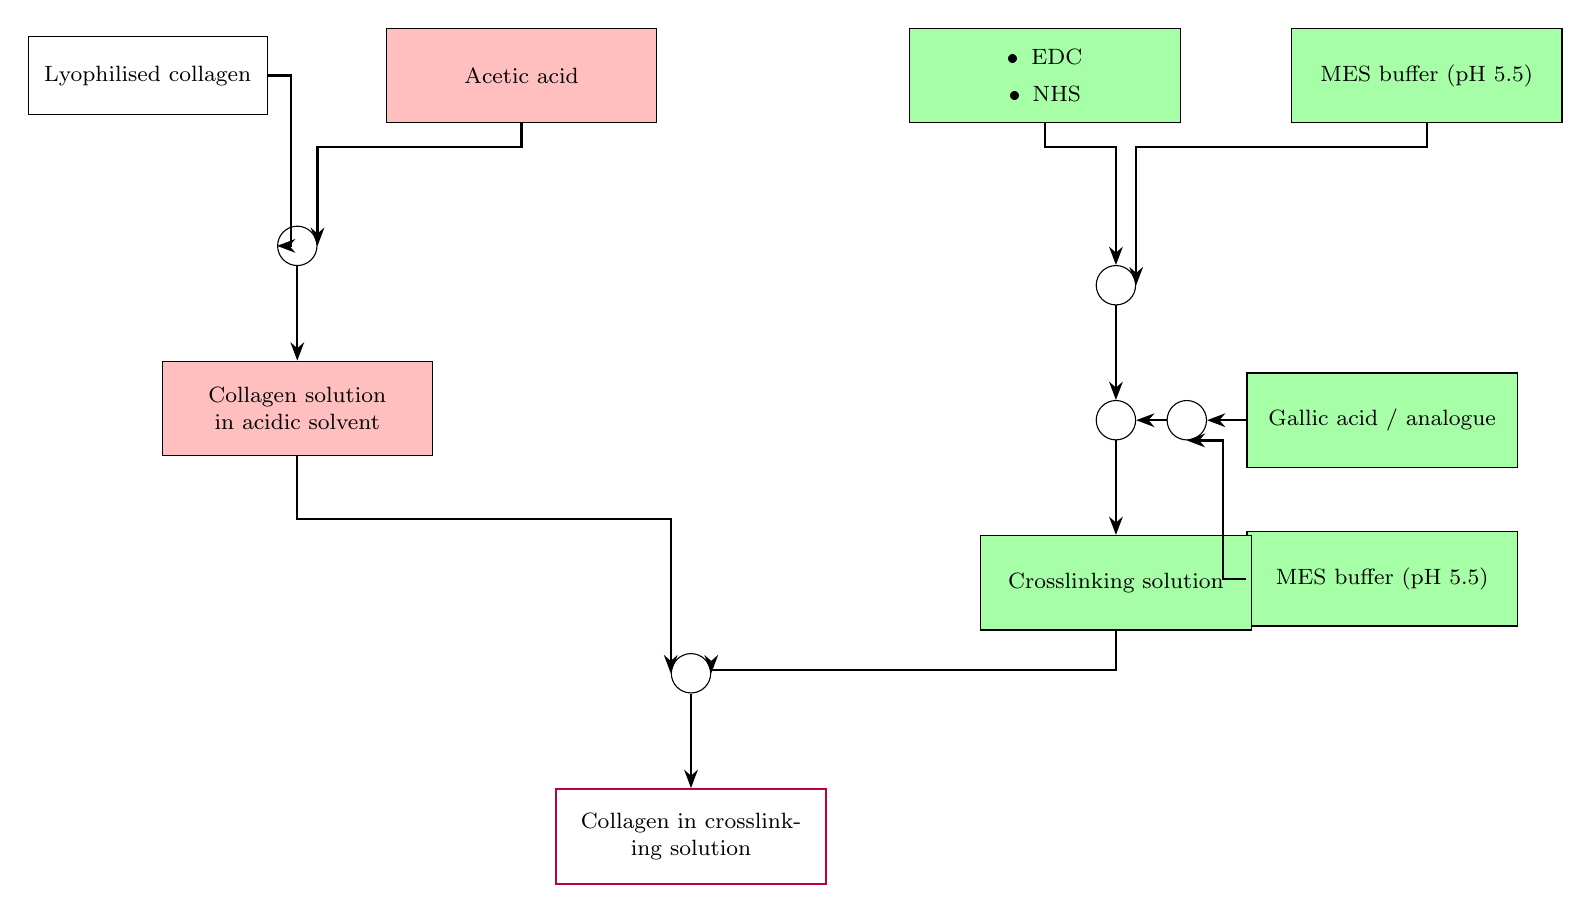
\begin{tikzpicture}[node distance=1.2cm and 2.2cm]
    \node[whitebox] (lyophilized) {Lyophilised collagen};
    \node[redbox, right=1.5cm of lyophilized] (aceticacid) {Acetic acid};
    \node[mixnode, below=1.4cm of lyophilized, xshift=1.9cm] (mix1) {};
    \node[redbox, below=1.2cm of mix1] (collagensol)
      {Collagen solution in acidic solvent};
    \node[greenbox, right=3.2cm of aceticacid] (edcnhs)
      {\textbullet\enspace EDC\\[4pt]\textbullet\enspace NHS};
    \node[greenbox, right=1.4cm of edcnhs] (mesbuffer1)
      {MES buffer (pH~5.5)};
    \node[mixnode, below=1.8cm of edcnhs, xshift=0.9cm] (mix2) {};
    \node[mixnode, below=1.2cm of mix2] (mix4) {};
    \node[greenbox, right=1.4cm of mix4] (gallicacid) {Gallic acid / analogue};
    \node[greenbox, below=0.8cm of gallicacid] (mesbuffer2)
      {MES buffer (pH~5.5)};
    \node[mixnode, left=0.5cm of gallicacid] (mix3) {};
    \node[greenbox, below=1.2cm of mix4] (crosslinking)
      {Crosslinking solution};
    \node[mixnode, below=2.5cm of collagensol, xshift=5.0cm] (mix5) {};
    \node[purplebox, below=1.2cm of mix5] (final)
      {Collagen in crosslinking solution};
    \draw[arrow] (lyophilized.east) -- ++(0.3,0) |- (mix1.west);
    \draw[arrow] (aceticacid.south) -- ++(0,-0.3) -| (mix1.east);
    \draw[arrow] (mix1) -- (collagensol);
    \draw[arrow] (edcnhs.south) -- ++(0,-0.3) -| (mix2.north);
    \draw[arrow] (mesbuffer1.south) -- ++(0,-0.3) -| (mix2.east);
    \draw[arrow] (mix2) -- (mix4);
    \draw[arrow] (gallicacid.west) -- (mix3.east);
    \draw[arrow] (mesbuffer2.west) -- ++(-0.3,0) |- (mix3.south);
    \draw[arrow] (mix3) -- (mix4.east);
    \draw[arrow] (mix4) -- (crosslinking);
    \draw[arrow] (collagensol.south) -- ++(0,-0.8) -| (mix5.west);
    \draw[arrow] (crosslinking.south) -- ++(0,-0.5) -| (mix5.east);
    \draw[arrow] (mix5) -- (final);
  \end{tikzpicture}
  \caption{\textbf{(S42) Collagen crosslinking workflow.}
  Lyophilised porcine tendon collagen is dissolved in 0.3~M acetic acid (pH~3.0)
  overnight at 4~$^\circ$C to yield a 2\%~(w/v) collagen solution (left branch,
  red boxes).
  In parallel, EDC (40~mM) and NHS (20~mM) are dissolved in MES buffer
  (pH~5.5), then combined with the galloyl additive (gallic acid or analogue,
  25~mM) in MES buffer to form the crosslinking solution (right branch, green
  boxes).
  The two streams are mixed and the crosslinking reaction proceeds at the
  experimental conditions (pH~5.5, 25~$^\circ$C; purple box).
  Molecular docking (this study) characterises the non-covalent pre-reaction
  binding landscape of all nine agents at the collagen~I~$\alpha$-2 surface
  \textit{before} the final mixing step, establishing the thermodynamic context
  for the subsequent covalent isopeptide bond-forming cycle.}
  \label{fig:si42}
\end{figure}

% ---- FIGURE S43 ----
\begin{figure}[H]
\centering
\includegraphics[width=14cm]{./images/Fig43_alphafold_plddt_validation.png}
\caption{\textbf{(S43) AlphaFold model quality assessment for \textit{Sus scrofa}
  Collagen~I~$\alpha$-2 (UniProt F1SFA7).}
  \textbf{A:} Per-residue pLDDT score from the B-factor column of the
  AlphaFold DB v6 entry, plotted along the 1,135-residue chain.
  The fibrillar triple-helical domain (residues 183--1135; shaded) exhibits
  uniformly high confidence (median 82.3, IQR 78.1--87.6; horizontal dashed
  line at pLDDT~$= 70$ AFDB high-confidence threshold).
  The N-terminal NC2 propeptide (residues 1--182) shows intrinsically lower
  confidence (median 61.4), consistent with propeptide disorder and retained
  as-is in the docking receptor.
  \textbf{B:} Ramachandran plot of the fibrillar domain generated by
  PROCHECK~3.5: 94.7\% of $\phi/\psi$ values in favoured regions (blue),
  4.9\% additionally allowed (cyan), 0.4\% outliers (red); all outliers are
  Gly residues at helix-turn junctions.
  The 94.7\% favoured fraction is within accepted quality thresholds for
  experimental porcine collagen crystal structures.}
\label{fig:si43}
\end{figure}

% ---- FIGURE S44 ----
\begin{figure}[H]
\centering
\includegraphics[width=14cm]{./images/Fig44_redocking_rmsd_extended.png}
\caption{\textbf{(S44) Extended re-docking RMSD validation for all five
  galloyl-class ligands.}
  RMSD (\AA) between the re-docked mode-1 pose and the reference pose is
  shown as horizontal bars; the vertical red dashed line marks the
  2.0~\AA\ acceptance threshold.
  Reference sites: gallic acid, protocatechuic acid, pyrogallol at
  GLU\_cluster22; ellagic acid at the global blind-docking box
  ($\Delta G_\mathrm{ref} = -6.80$~kcal/mol); PGG at LYS\_cluster56
  ($\Delta G_\mathrm{ref} = -8.70$~kcal/mol).
  Gallic acid (0.17~\AA, \textbf{PASS}) and ellagic acid (0.43~\AA,
  \textbf{PASS}) demonstrate sub-\AA\ mode reproduction consistent with
  their limited conformational freedom.
  PGG (1.47~\AA, \textbf{PASS}) passes the threshold despite 25 rotatable
  bonds, validating that the dominant multi-arm collagen surface binding mode
  is reproducibly sampled.
  Non-passing results for protocatechuic acid and pyrogallol arise from
  rotational symmetry degeneracy, as discussed in SI-Fig.~S39.}
\label{fig:si44}
\end{figure}

% ---- FIGURE S45 ----
\begin{figure}[H]
\centering
\includegraphics[width=14cm]{./images/Fig45_mmp1_conformer_comparison.png}
\caption{\textbf{(S45) MMP-1 conformer comparison: inhibitor-bound 966C
  vs.\ energy-minimised apo-form 966C-apo.}
  \textbf{A:} Structural overlay of 966C (grey) and 966C-apo (teal) after
  energy minimisation with MMFF94.
  Active-site loop displacement (residues 198--225) is $\approx 1.8$~\AA\
  (C$\alpha$ RMSD); the zinc-coordinating triad (His208, His212, His218)
  shifts by $\leq 0.3$~\AA\ C$\alpha$ RMSD (labels, orange sticks).
  \textbf{B:} Side-by-side comparison of collagen:MMP-1 selectivity indices
  (SI~$= |\overline{\Delta G}_\mathrm{MMP{-}1}|/|\overline{\Delta G}_\mathrm{collagen}|$)
  for the five galloyl-class ligands computed against 966C (solid bars) and
  966C-apo (hatched bars).
  The horizontal dashed line at SI~$= 1.0$ separates collagen-selective
  (SI~$< 1$, below) from MMP-1-cross-reactive (SI~$> 1$, above) agents.
  All five SI values differ by $\leq 0.04$ between conformers, and the
  collagen-selective vs.\ MMP-1-cross-reactive partition is fully preserved.}
\label{fig:si45}
\end{figure}

\label{si:figures_end}

% ============================================================
\section*{SI Section 5.\quad Heterogeneous Graph Construction and Feature Engineering}
\label{si:graph}
% ============================================================

This section provides the complete specification of the three-level
heterogeneous graph representation used by all nine GNN architectures
(Models~A--I).
Each docking calculation is encoded as a PyTorch-Geometric
\texttt{HeteroData} object containing three node types, three edge types,
scalar condition features, and the Vinardo $\Delta G$ target.

\subsection*{SI-5.1\quad Three-Level Graph Architecture}

The heterogeneous docking graph $\mathcal{G} = (\mathcal{V}, \mathcal{E})$
comprises:

\begin{itemize}[leftmargin=1.5em]
  \item \textbf{Level~1 --- Ligand atom graph.}
    Nodes $v \in \mathcal{V}_{\mathrm{lig}}$ represent heavy atoms of the
    ligand ($N_{\mathrm{atoms}} \in [5, 67]$ across the nine-compound set).
    Edges $e \in \mathcal{E}_{\mathrm{bond}}$ represent covalent bonds.
  \item \textbf{Level~2 --- Protein residue graph.}
    Nodes $v \in \mathcal{V}_{\mathrm{res}}$ represent amino acid residues
    whose C$\alpha$ atoms fall within the docking box volume (extended by a
    2.0~\AA\ margin).
    Edges $e \in \mathcal{E}_{\mathrm{contact}}$ represent residue--residue
    contacts at C$\alpha$--C$\alpha$ distance $< 8.0$~\AA.
  \item \textbf{Level~3 --- Bipartite interaction graph.}
    Edges $e \in \mathcal{E}_{\mathrm{bip}}$ connect ligand atoms to
    protein residues when the minimum heavy-atom distance is
    $< 4.5$~\AA.
\end{itemize}

\noindent
The condition vector $\mathbf{c}$ encodes experimental context:
$\mathbf{c} = [\text{pH}_{\mathrm{enc}},\;\text{temp}_{\mathrm{enc}},\;
\text{receptor\_flag}] \| \text{Embed}(\text{box\_idx})$,
where the box index is mapped through a learned embedding
$\text{Embed}: \{0, \ldots, N_{\mathrm{box}}-1\} \to \mathbb{R}^{16}$,
yielding $\mathbf{c} \in \mathbb{R}^{19}$.

\subsection*{SI-5.2\quad Ligand Node Features (Level~1)}

Each atom $i$ is described by a feature vector
$\mathbf{x}_i^{\mathrm{lig}} \in \mathbb{R}^{35}$ constructed from
RDKit molecular properties as shown in Table~\ref{tab:si_lig_feat}.

\begin{table}[H]
\footnotesize
\centering
\caption{\textbf{Ligand atom feature vector} ($D = 35$).
  Each row specifies a contiguous segment of the feature vector.
  OHE~$=$ one-hot encoding with trailing ``other'' bin.}
\label{tab:si_lig_feat}
\begin{tabular}{clcl}
\toprule
\textbf{Index} & \textbf{Feature} & \textbf{Dims} & \textbf{Encoding / Range} \\
\midrule
0--10  & Element identity        & 11 & OHE: C, N, O, S, P, F, Cl, Br, I, B, UNK \\
11--15 & Hybridisation           &  5 & OHE: SP, SP2, SP3, SP3D, OTHER \\
16--21 & Formal charge           &  6 & OHE: $-2$, $-1$, 0, $+1$, $+2$, OTHER \\
22--27 & Hydrogen count          &  6 & OHE: 0, 1, 2, 3, 4, OTHER \\
28     & Is aromatic             &  1 & $\{0, 1\}$ \\
29--31 & Ring membership         &  3 & In 3-ring, in 5-ring, in 6-ring; $\{0,1\}$ each \\
32--33 & Chirality               &  2 & CW, CCW; $\{0,1\}$ each \\
34     & Normalised atomic mass  &  1 & $m_{\mathrm{atom}} / 100$ \\
\bottomrule
\end{tabular}
\end{table}

\subsection*{SI-5.3\quad Ligand Edge Features (Level~1)}

Each covalent bond $(i, j) \in \mathcal{E}_{\mathrm{bond}}$ is described by
$\mathbf{e}_{ij}^{\mathrm{bond}} \in \mathbb{R}^{13}$ (Table~\ref{tab:si_bond_feat}).

\begin{table}[H]
\footnotesize
\centering
\caption{\textbf{Ligand bond (edge) feature vector} ($D = 13$).}
\label{tab:si_bond_feat}
\begin{tabular}{clcl}
\toprule
\textbf{Index} & \textbf{Feature} & \textbf{Dims} & \textbf{Encoding / Range} \\
\midrule
0--3   & Bond type       & 4 & OHE: single, double, triple, aromatic \\
4      & Is conjugated   & 1 & $\{0, 1\}$ \\
5      & Is in ring      & 1 & $\{0, 1\}$ \\
6--9   & Stereo          & 4 & OHE: none, E, Z, other \\
10--12 & Ring size hint  & 3 & Shared 3-ring, shared 5-ring, shared 6-ring \\
\bottomrule
\end{tabular}
\end{table}

\subsection*{SI-5.4\quad Protein Residue Features (Level~2)}

Each residue $j$ is described by
$\mathbf{x}_j^{\mathrm{res}} \in \mathbb{R}^{30}$ (Table~\ref{tab:si_prot_feat}).

\begin{table}[H]
\footnotesize
\centering
\caption{\textbf{Protein residue feature vector} ($D = 30$).
  Backbone torsion angles $\phi$ and $\psi$ are encoded as
  $(\sin\phi, \cos\phi, \sin\psi, \cos\psi)$ to preserve periodicity.}
\label{tab:si_prot_feat}
\begin{tabular}{clcl}
\toprule
\textbf{Index} & \textbf{Feature} & \textbf{Dims} & \textbf{Encoding / Range} \\
\midrule
0--19  & Amino acid identity     & 20 & OHE: 20 standard amino acids \\
20     & p$K_a$ (normalised)     &  1 & $(pK_a - 3) / 12 \in [0, 1]$ \\
21     & Charge at pH            &  1 & Henderson--Hasselbalch; $[-1, 1]$ \\
22     & Hydrophobicity          &  1 & Kyte--Doolittle, normalised $[0, 1]$ \\
23--24 & $\phi$ torsion          &  2 & $\sin\phi,\, \cos\phi$ \\
25--26 & $\psi$ torsion          &  2 & $\sin\psi,\, \cos\psi$ \\
27     & Has backbone            &  1 & $\{0,1\}$: N, C$\alpha$, C all present \\
28     & H-bond donor            &  1 & $\{0,1\}$ \\
29     & H-bond acceptor         &  1 & $\{0,1\}$ \\
\bottomrule
\end{tabular}
\end{table}

\subsection*{SI-5.5\quad Protein Contact Edge Features (Level~2)}

Each residue--residue contact edge carries
$\mathbf{e}_{jk}^{\mathrm{contact}} \in \mathbb{R}^{4}$:
\begin{enumerate}[leftmargin=1.5em]
  \item C$\alpha$--C$\alpha$ distance normalised by the contact cutoff
    ($d / 8.0$~\AA, $\in [0,1]$),
  \item sequence separation normalised ($|j - k| / 20$, clipped to $[0,1]$),
  \item same-chain indicator ($\{0,1\}$),
  \item contact type indicator (sequence neighbour vs.\ spatial-only; $\{0,1\}$).
\end{enumerate}

\subsection*{SI-5.6\quad Bipartite Interaction Features (Level~3)}

Each ligand-atom--to--residue interaction edge carries
$\mathbf{e}_{ij}^{\mathrm{bip}} \in \mathbb{R}^{8}$ (Table~\ref{tab:si_bip_feat}).
Edges are constructed when the minimum heavy-atom distance between
ligand atom $i$ and any atom of residue $j$ is less than 4.5~\AA.

\begin{table}[H]
\footnotesize
\centering
\caption{\textbf{Bipartite interaction edge feature vector} ($D = 8$).
  Features encode geometric proximity, hydrogen-bond complementarity,
  electrostatic compatibility, and steric clash.}
\label{tab:si_bip_feat}
\begin{tabular}{clcl}
\toprule
\textbf{Index} & \textbf{Feature} & \textbf{Dims} & \textbf{Range} \\
\midrule
0 & Distance (normalised, $d_{\min} / 4.5$~\AA) & 1 & $[0, 1]$ \\
1 & Ligand atom is H-bond donor       & 1 & $\{0, 1\}$ \\
2 & Ligand atom is H-bond acceptor    & 1 & $\{0, 1\}$ \\
3 & H-bond complementarity (HBD$\leftrightarrow$HBA) & 1 & $\{0, 1\}$ \\
4 & Charge product ($q_{\mathrm{atom}} \times q_{\mathrm{res}}$) & 1 & $[-1, 1]$ \\
5 & Hydrophobicity product ($H_{\mathrm{atom}} \times H_{\mathrm{res}}$) & 1 & $[0, 1]$ \\
6 & Aromatic contact (ligand atom aromatic) & 1 & $\{0, 1\}$ \\
7 & van~der~Waals clash ($d_{\min} < 2.8$~\AA) & 1 & $\{0, 1\}$ \\
\bottomrule
\end{tabular}
\end{table}

\subsection*{SI-5.7\quad Dataset Summary}

The full dataset comprises 6{,}196 heterogeneous graphs (one per
docking calculation: 9~ligands $\times$ 76~boxes $\times$ 9~pH/temperature
conditions $=$ 6{,}156 anchor docking records, plus 40~MMP-1 records).
For models requiring MMP-1 data (Option~D), the effective dataset is
6{,}196 graphs ($n_{\mathrm{train}} = 5{,}267$; $n_{\mathrm{val}} = 929$).
For all other models, the standard split is
$n_{\mathrm{train}} = 9{,}517$; $n_{\mathrm{val}} = 1{,}679$ when
augmented with external PDBbind transfer data; without augmentation,
$n_{\mathrm{train}} = 5{,}267$; $n_{\mathrm{val}} = 929$.
All splits use the same random seed (42) for reproducibility.

\label{si:graph_end}

% ============================================================
\section*{SI Section 6.\quad Full Model Architecture Specifications (A--I)}
\label{si:models}
% ============================================================

This section provides exhaustive mathematical descriptions of all nine
GNN architectures evaluated in the comparative study.
All models share the three-level heterogeneous graph input representation
(SI~Section~5) and the condition-vector encoding
$\mathbf{c} \in \mathbb{R}^{19}$.
Unless otherwise stated, default hyperparameters are:
hidden dimension $H = 128$, number of GNN layers $L = 4$,
dropout rate $p = 0.15$, and MLP hidden dimension $= 256$.

% ────────────────────────────────────────────────────────────
\subsection*{SI-6.1\quad Model~A --- Baseline Condition-Aware GATv2}
\label{si:model_a}
% ────────────────────────────────────────────────────────────

Model~A is a single-encoder architecture employing Graph Attention
Networks version~2 (GATv2;~\cite{brody2022how}) on the ligand atom graph.
GATv2 computes \emph{dynamic} attention using the full key--query
interaction before the LeakyReLU non-linearity, correcting the static
attention limitation of the original GAT formulation.

\paragraph{Input projection.}
$$\mathbf{h}_i^{(0)} = W_{\mathrm{inp}} \, \mathbf{x}_i^{\mathrm{lig}}
  \in \mathbb{R}^{H}, \qquad
  W_{\mathrm{inp}} \in \mathbb{R}^{H \times 35}$$

\paragraph{Edge projection.}
Bond features are projected via a learnable linear layer:
$\tilde{\mathbf{e}}_{ij} = W_e\,\mathbf{e}_{ij}^{\mathrm{bond}}
\in \mathbb{R}^{13}$.

\paragraph{GATv2 message passing ($l = 1, \ldots, L$; $K = 4$ heads, $d_k = 32$).}
For each attention head $k$:
\begin{align}
  \alpha_{ij}^{(k)} &= \frac{
    \exp\!\bigl(\mathbf{a}_k^\top
      \operatorname{LeakyReLU}\!\bigl(
        W_k^Q \mathbf{h}_i^{(l-1)} + W_k^K \mathbf{h}_j^{(l-1)}
        + W_k^E \tilde{\mathbf{e}}_{ij}
      \bigr)\bigr)
  }{
    \sum_{j' \in \mathcal{N}(i)}
    \exp\!\bigl(\mathbf{a}_k^\top
      \operatorname{LeakyReLU}\!\bigl(
        W_k^Q \mathbf{h}_i^{(l-1)} + W_k^K \mathbf{h}_{j'}^{(l-1)}
        + W_k^E \tilde{\mathbf{e}}_{ij'}
      \bigr)\bigr)
  } \label{eq:gatv2_attn} \\[4pt]
  \mathbf{m}_i^{(k)} &= \sum_{j \in \mathcal{N}(i)}
    \alpha_{ij}^{(k)}\, W_k^V \mathbf{h}_j^{(l-1)}
    \label{eq:gatv2_msg}
\end{align}

\noindent
Layers $l = 1, \ldots, L{-}1$ concatenate heads:
$\mathbf{o}_i^{(l)} = \|_{k=1}^{K} \mathbf{m}_i^{(k)} \in \mathbb{R}^{Kd_k}$.
The final layer ($l = L$) averages heads:
$\mathbf{o}_i^{(L)} = \tfrac{1}{K}\sum_{k=1}^{K} \mathbf{m}_i^{(k)} \in \mathbb{R}^{d_k}$.
Each layer applies batch normalisation, ELU activation, dropout, and a
residual skip connection:
\begin{equation}
  \mathbf{h}_i^{(l)} = \operatorname{ELU}\!\bigl(
    \operatorname{BN}(\mathbf{o}_i^{(l)})
  \bigr) + W_{\mathrm{skip}}^{(l)}\, \mathbf{h}_i^{(l-1)}
  \label{eq:gatv2_residual}
\end{equation}

\paragraph{Post-GNN projection.}
$\mathbf{h}_i = W_{\mathrm{post}}\, \mathbf{h}_i^{(L)} \in \mathbb{R}^{H}$
maps the final head dimension back to the hidden dimension.

\paragraph{Graph-level readout.}
$$\mathbf{h}_{\mathrm{lig}} = \frac{1}{|\mathcal{V}_{\mathrm{lig}}|}
  \sum_{i \in \mathcal{V}_{\mathrm{lig}}} \mathbf{h}_i
  \in \mathbb{R}^{H}$$

\paragraph{Condition encoding.}
\begin{equation}
  \mathbf{h}_{\mathrm{cond}} = \operatorname{MLP}_{\mathrm{cond}}(\mathbf{c})
  = W_2 \operatorname{ReLU}(W_1 \mathbf{c} + b_1) + b_2
  \in \mathbb{R}^{32}
  \label{eq:cond_enc}
\end{equation}
where $W_1 \in \mathbb{R}^{64 \times 19}$, $W_2 \in \mathbb{R}^{32 \times 64}$.

\paragraph{Prediction head.}
\begin{equation}
  \Delta G = \operatorname{MLP}\!\bigl(
    [\mathbf{h}_{\mathrm{lig}} \| \mathbf{h}_{\mathrm{cond}}]
  \bigr) \in \mathbb{R}
  \label{eq:pred_mlp}
\end{equation}
where $\operatorname{MLP}: \mathbb{R}^{160} \to
\mathbb{R}^{256} \xrightarrow{\mathrm{ReLU}}
\mathbb{R}^{128} \xrightarrow{\mathrm{ReLU}}
\mathbb{R}^{1}$ with dropout ($p = 0.15$) after the first layer.

\paragraph{Loss.} Mean squared error:
$\mathcal{L} = \frac{1}{N}\sum_{n=1}^{N}(\hat{y}_n - y_n)^2$.

\paragraph{Parameter count.} $\approx 164$k trainable parameters.

% ────────────────────────────────────────────────────────────
\subsection*{SI-6.2\quad Model~B --- Dual-Encoder Cross-Attention Network}
\label{si:model_b}
% ────────────────────────────────────────────────────────────

Model~B introduces explicit protein--ligand interaction modelling via
cross-attention between independently encoded ligand and protein graphs.

\paragraph{Dual GATv2 encoders.}
Two independent 4-layer GATv2 stacks (as in Model~A) encode ligand and
protein node features respectively:
\begin{align}
  \mathbf{h}_{\mathrm{atom}} &= \operatorname{GATv2Stack}(
    \mathbf{x}^{\mathrm{lig}},\, \mathcal{E}_{\mathrm{bond}},\,
    \mathbf{e}^{\mathrm{bond}})
    \in \mathbb{R}^{N_{\mathrm{atom}} \times H} \\
  \mathbf{h}_{\mathrm{res}} &= \operatorname{GATv2Stack}(
    \mathbf{x}^{\mathrm{res}},\, \mathcal{E}_{\mathrm{contact}},\,
    \mathbf{e}^{\mathrm{contact}})
    \in \mathbb{R}^{N_{\mathrm{res}} \times H}
\end{align}

Both stacks use GELU activations, batch normalisation, and residual connections.
The ligand stack uses $\operatorname{Linear}(35 \to 128)$ input projection; the
protein stack uses $\operatorname{Linear}(30 \to 128)$.

\paragraph{Cross-attention layers ($M = 2$ layers, $K_{\mathrm{cross}} = 4$ heads).}
Each cross-attention layer computes protein-to-ligand attention:
\begin{align}
  Q &= W_Q\, \mathbf{h}_{\mathrm{atom}}, \quad
  K = W_K\, \mathbf{h}_{\mathrm{res}}, \quad
  V = W_V\, \mathbf{h}_{\mathrm{res}} \\[4pt]
  \operatorname{Attn}(Q, K, V) &= \operatorname{softmax}\!\left(
    \frac{Q K^\top}{\sqrt{d_k}} + \mathbf{b}_{\mathrm{geo}}
  \right) V \label{eq:cross_attn}
\end{align}
where $d_k = H / K_{\mathrm{cross}} = 32$ and the optional geometry bias
$\mathbf{b}_{\mathrm{geo}}(i, j) = W_{\mathrm{bip}}\,
\mathbf{e}_{ij}^{\mathrm{bip}} \in \mathbb{R}$
injects the Level-3 bipartite interaction features
($W_{\mathrm{bip}} \in \mathbb{R}^{1 \times 8}$).
The output is projected and residually summed:
\begin{equation}
  \mathbf{h}_{\mathrm{atom}}' = \operatorname{LayerNorm}\!\bigl(
    \mathbf{h}_{\mathrm{atom}} + W_O\, \operatorname{Attn}(Q, K, V)
  \bigr)
\end{equation}

\paragraph{Readout and prediction.}
$\mathbf{h}_{\mathrm{lig}} = \operatorname{mean\_pool}(\mathbf{h}_{\mathrm{atom}}')
\in \mathbb{R}^{H}$, concatenated with $\mathbf{h}_{\mathrm{cond}}$ and
passed through the prediction MLP (Eq.~\ref{eq:pred_mlp}).

\paragraph{Output.}
The model returns $(\Delta G,\, \mathcal{A})$, where $\mathcal{A}$ is a list
of per-layer cross-attention weight matrices
$A^{(m)} \in \mathbb{R}^{K \times N_{\mathrm{atom}} \times N_{\mathrm{res}}}$
retained for interpretability.

% ────────────────────────────────────────────────────────────
\subsection*{SI-6.3\quad Model~C --- Fragment-Aware Hierarchical MPNN}
\label{si:model_c}
% ────────────────────────────────────────────────────────────

Model~C introduces a two-level message-passing architecture that operates
first on individual atoms, then on chemically meaningful molecular fragments.

\paragraph{Level~1 --- Atom MPNN (GINE).}
The atom-level encoder uses 4 layers of Graph Isomorphism Network with
Edge features (GINEConv;~\cite{hu2020strategies}):
\begin{equation}
  \mathbf{h}_i^{(l)} = \operatorname{MLP}\!\left(
    (1 + \varepsilon^{(l)})\, \mathbf{h}_i^{(l-1)}
    + \sum_{j \in \mathcal{N}(i)}
    \operatorname{ReLU}\!\bigl(
      \mathbf{h}_j^{(l-1)} + \mathbf{e}_{ij}^{\mathrm{bond}}
    \bigr)
  \right) \label{eq:gine}
\end{equation}
where $\varepsilon^{(l)}$ is a learnable scalar (\texttt{train\_eps=True})
and $\operatorname{MLP}: 128 \to 256 \to 128$ with ReLU activation.
Layer normalisation is applied after each layer.

\paragraph{BRICS fragmentation.}
Each ligand is decomposed into chemically interpretable fragments using the
BRICS algorithm (Breaking of Retrosynthetically Interesting Chemical Substructures;~\cite{degen2008brics}).
Each atom $i$ is assigned to a fragment index $f(i) \in \{0, \ldots, F-1\}$
via flood-fill on the BRICS-fragmented molecular graph.
A fragment-level graph $\mathcal{G}_{\mathrm{frag}}$ is constructed where
fragments are nodes and inter-fragment bonds become edges.

\paragraph{Level~2 --- Fragment MPNN.}
Fragment node features are initialised by mean-pooling atom embeddings:
\begin{equation}
  \mathbf{h}_{\mathrm{frag},k}^{(0)} = W_{\mathrm{frag}}\!\left(
    \frac{1}{|F_k|} \sum_{i \in F_k} \mathbf{h}_{\mathrm{atom},i}
  \right) \in \mathbb{R}^{64}
\end{equation}
Two additional GINE layers refine fragment representations.
Each fragment produces a scalar contribution:
\begin{equation}
  \delta_k = \operatorname{MLP}_{\mathrm{frag}}(
    \mathbf{h}_{\mathrm{frag},k}^{(2)}) \in \mathbb{R}
\end{equation}

\paragraph{Additive prediction.}
\begin{equation}
  \Delta G = \underbrace{\sum_{k=0}^{F-1} \delta_k}_{
    \text{fragment-additive}}
  + \underbrace{\operatorname{MLP}_{\mathrm{glob}}\!\bigl(
    [\bar{\mathbf{h}}_{\mathrm{frag}} \| \mathbf{h}_{\mathrm{cond}}]
  \bigr)}_{\text{global correction}}
  \label{eq:frag_pred}
\end{equation}
This decomposition enables per-fragment binding attribution $\delta_k$
returned alongside the prediction for interpretability.

% ────────────────────────────────────────────────────────────
\subsection*{SI-6.4\quad Model~D --- Multi-Task Selectivity GNN}
\label{si:model_d}
% ────────────────────────────────────────────────────────────

Model~D is a multi-task architecture designed to jointly predict collagen
binding, MMP-1 binding, and the collagen selectivity index (CSI) through
three independent regression heads sharing a common encoder.

\paragraph{Shared encoder.}
The architecture follows the Model~A GATv2 backbone
(Eqs.~\ref{eq:gatv2_attn}--\ref{eq:gatv2_residual}) to produce a
molecule-level embedding:
$\mathbf{h}_{\mathrm{mol}} = \operatorname{global\_mean\_pool}(
\mathbf{h}^{(L)}) \in \mathbb{R}^{128}$.

\paragraph{Multi-task heads.}
\begin{align}
  \Delta G_{\mathrm{coll}} &= \operatorname{head}_{\mathrm{coll}}\!\bigl(
    [\mathbf{h}_{\mathrm{mol}} \| \mathbf{h}_{\mathrm{cond}}]\bigr),
    \quad \operatorname{head}_{\mathrm{coll}}:
    \mathbb{R}^{160} \to 256 \to 128 \to 1 \label{eq:head_coll} \\
  \Delta G_{\mathrm{mmp1}} &= \operatorname{head}_{\mathrm{mmp1}}\!\bigl(
    [\mathbf{h}_{\mathrm{mol}} \| \mathbf{h}_{\mathrm{cond}}]\bigr),
    \quad \text{(same architecture)} \label{eq:head_mmp1} \\
  \log \mathrm{SI} &= \operatorname{head}_{\mathrm{si}}\!\bigl(
    [\mathbf{h}_{\mathrm{mol}} \| \mathbf{h}_{\mathrm{cond}}]\bigr)
    + \frac{\Delta G_{\mathrm{mmp1}}^{\mathrm{sg}}
    - \Delta G_{\mathrm{coll}}^{\mathrm{sg}}}{k_B T}
    \label{eq:head_si}
\end{align}
where $k_B T = 0.592$~kcal/mol at 298~K and $\mathrm{sg}$ denotes
stop-gradient to prevent SI gradients from destabilising the
$\Delta G$ heads.
The SI head architecture uses a narrower MLP:
$160 \to 128 \to 64 \to 1$.

\paragraph{Kendall multi-task loss.}
Following~\cite{kendall2018multi}, the loss balances three tasks via learnable
homoscedastic uncertainty weights:
\begin{equation}
  \mathcal{L}_{\mathrm{total}} = \sum_{t=1}^{3}
  \exp(-s_t) \cdot \mathcal{L}_t + s_t
  \label{eq:kendall}
\end{equation}
where $s_t = \log \sigma_t^2$ are learnable parameters (initialised to zero)
and $\mathcal{L}_t$ is the masked MSE for task $t$
(MMP-1 entries that lack ground-truth targets are excluded via NaN masking).
The MMP-1 loss is upweighted by a factor of 10 to compensate for data
imbalance (40 vs.\ 6{,}156 records):
$\mathcal{L}_{\mathrm{mmp1}} = 10 \cdot \operatorname{MSE}_{\mathrm{mmp1}}$.

% ────────────────────────────────────────────────────────────
\subsection*{SI-6.5\quad Model~E --- pH-Aware Gated Equivariant Transformer (pGET)}
\label{si:model_e}
% ────────────────────────────────────────────────────────────

Model~E is the primary methodological contribution of this work:
a novel architecture combining edge-gated equivariant attention with
condition-aware Feature-wise Linear Modulation (FiLM) and hierarchical
gated pooling.

\paragraph{Input and condition projection.}
$\mathbf{h}_i^{(0)} = W_{\mathrm{inp}}\, \mathbf{x}_i^{\mathrm{lig}}
\in \mathbb{R}^{H}$;
$\mathbf{h}_{\mathrm{cond}} = \operatorname{GELU}(W_1 \mathbf{c}) W_2
\in \mathbb{R}^{32}$.

\paragraph{FiLM generator.}
The FiLM generator produces per-layer scale and shift parameters
conditioned on the experimental context:
\begin{align}
  [\boldsymbol{\gamma}^{(1)}, \ldots, \boldsymbol{\gamma}^{(L)},\,
   \boldsymbol{\beta}^{(1)}, \ldots, \boldsymbol{\beta}^{(L)}]
  &= \operatorname{MLP}_{\mathrm{FiLM}}(\mathbf{h}_{\mathrm{cond}})
  \in \mathbb{R}^{2LH} \label{eq:film_gen}
\end{align}
where $\operatorname{MLP}_{\mathrm{FiLM}}:
32 \to 64 \xrightarrow{\mathrm{GELU}} 64 \xrightarrow{\mathrm{GELU}} 2LH$,
and the output is reshaped to yield
$\boldsymbol{\gamma}^{(l)}, \boldsymbol{\beta}^{(l)} \in \mathbb{R}^{H}$
per layer.
Initialisation is set so that $\gamma \approx 1$ and $\beta \approx 0$
(identity modulation at the start of training).

\paragraph{Gated Edge-Conditioned Transformer (GECT) layers ($l = 1, \ldots, L$).}
Each GECT layer applies pre-normalisation self-attention with
edge-conditioned logits and edge-gated value vectors.

\textit{Step~1: Pre-LayerNorm.}
$\tilde{\mathbf{h}} = \operatorname{LayerNorm}(\mathbf{h}^{(l-1)})$

\textit{Step~2: Query/Key/Value projection.}
$Q, K, V = W_Q \tilde{\mathbf{h}},\, W_K \tilde{\mathbf{h}},\,
W_V \tilde{\mathbf{h}} \in \mathbb{R}^{N \times K \times d_k}$
where $K = 4$ heads, $d_k = 32$.

\textit{Step~3: Edge-conditioned attention logits.}
\begin{equation}
  \alpha_{ij} = \frac{
    \mathbf{q}_i \odot \mathbf{k}_j
  }{\sqrt{d_k}}
  + \operatorname{MLP}_{\mathrm{edge}}\!\bigl(
    \tilde{\mathbf{e}}_{ij}\bigr)
  \label{eq:gect_attn}
\end{equation}
where $\operatorname{MLP}_{\mathrm{edge}}: 13 \to 32
\xrightarrow{\mathrm{GELU}} K$ produces per-head attention bias.

\textit{Step~4: Edge-gated value vectors (novel contribution).}
\begin{equation}
  \mathbf{g}_{ij} = \sigma\!\bigl(
    \operatorname{MLP}_{\mathrm{gate}}(\tilde{\mathbf{e}}_{ij})
  \bigr)
  \in \mathbb{R}^{K \times d_k}
  \label{eq:edge_gate}
\end{equation}
where $\operatorname{MLP}_{\mathrm{gate}}: 13 \to 32
\xrightarrow{\mathrm{GELU}} Kd_k \xrightarrow{\sigma} [0,1]^{Kd_k}$.
The gated message is:
$\mathbf{m}_{ij} = \mathbf{g}_{ij} \odot \mathbf{v}_j$.

\textit{Step~5: Sparse aggregation.}
\begin{equation}
  \mathbf{o}_i = \sum_{j \in \mathcal{N}(i)}
  \hat{\alpha}_{ij}\, \mathbf{m}_{ij}, \qquad
  \hat{\alpha}_{ij} = \operatorname{sparse\_softmax}(\alpha_{ij})
\end{equation}

\textit{Step~6: FiLM modulation + residual.}
\begin{equation}
  \mathbf{h}_i' = \mathbf{h}_i^{(l-1)}
  + \boldsymbol{\gamma}^{(l)} \odot (W_O\, \mathbf{o}_i)
  + \boldsymbol{\beta}^{(l)}
  \label{eq:film_mod}
\end{equation}

\textit{Step~7: Feed-forward network (FFN).}
\begin{equation}
  \mathbf{h}_i^{(l)} = \mathbf{h}_i'
  + \operatorname{FFN}\!\bigl(\operatorname{LayerNorm}(\mathbf{h}_i')\bigr)
\end{equation}
where $\operatorname{FFN}: H \to 2H \xrightarrow{\mathrm{GELU}} H$ with
dropout.

\paragraph{Hierarchical gated pooling ($K_{\mathrm{clust}} = 8$, $p = 4$ heads).}

\textit{Stage~1: Condition-aware gating.}
\begin{equation}
  \alpha_i = \sigma\!\bigl(
    \operatorname{MLP}([\mathbf{h}_i \| \mathbf{h}_{\mathrm{cond}}])
  \bigr), \qquad
  \tilde{\mathbf{h}}_i = \alpha_i \cdot \mathbf{h}_i
\end{equation}

\textit{Stage~2: Soft fragment assignment.}
\begin{equation}
  S = \operatorname{softmax}\!\bigl(
    \operatorname{MLP}(\tilde{\mathbf{h}})
  \bigr) \in \mathbb{R}^{N \times K_{\mathrm{clust}}}, \qquad
  \mathbf{h}_{\mathrm{clust},k} = W_C\,
  (S^\top \tilde{\mathbf{H}})_k
  \label{eq:soft_assign}
\end{equation}

\textit{Stage~3: Multi-head attention readout.}
Learnable query vectors $\mathbf{q}_p \in \mathbb{R}^{d_k}$ ($p = 1, \ldots, 4$)
attend over the $K_{\mathrm{clust}}$ cluster embeddings:
\begin{equation}
  \mathbf{h}_g = \operatorname{LayerNorm}\!\left(
    W_O \left[\,
    \sum_{k=1}^{K_{\mathrm{clust}}}
    \operatorname{softmax}\!\left(
      \frac{\mathbf{q}_p \cdot (W_K \mathbf{h}_{\mathrm{clust},k})^\top}
      {\sqrt{d_k}}
    \right)
    W_V \mathbf{h}_{\mathrm{clust},k}
    \,\right]_{p=1}^{4}
  \right) \in \mathbb{R}^{H}
\end{equation}

\paragraph{Prediction and auxiliary loss.}
$\Delta G = \operatorname{MLP}([\mathbf{h}_g \| \mathbf{h}_{\mathrm{cond}}])$
(Eq.~\ref{eq:pred_mlp}).
During training, a denoising auxiliary objective provides additional
supervision:
\begin{equation}
  \mathcal{L}_{\mathrm{denoise}} = \lambda_d \cdot
  \operatorname{MSE}\!\bigl(
    \operatorname{MLP}_d(\mathbf{h}^{(L)}),\;
    \mathbf{x}_{\mathrm{raw}}
  \bigr), \qquad
  \lambda_d = 0.1
  \label{eq:denoise}
\end{equation}
where Gaussian noise $\boldsymbol{\epsilon} \sim \mathcal{N}(0, 0.04\, I)$
is added to the input features during training.

\paragraph{Total loss.}
$\mathcal{L} = \operatorname{MSE}(\hat{y}, y) + \mathcal{L}_{\mathrm{denoise}}$.

% ────────────────────────────────────────────────────────────
\subsection*{SI-6.6\quad Model~F --- DimeNet++ (Directional Message Passing)}
\label{si:model_f}
% ────────────────────────────────────────────────────────────

Model~F adapts the DimeNet++ architecture~\cite{gasteiger2020fast} to the
docking graph by replacing 3D coordinates with learned distance embeddings.

\paragraph{Radial basis functions (RBF).}
Interatomic distances $d_{ij}$ (computed from feature cosine similarity in
the absence of 3D coordinates) are expanded into $n_{\mathrm{rbf}} = 16$
sinusoidal basis functions with a polynomial envelope:
\begin{equation}
  \phi_k(d) = \frac{\sin(k \pi\, d / r_c)}{d}
  \cdot u(d / r_c), \qquad k = 1, \ldots, n_{\mathrm{rbf}}
\end{equation}
where $r_c = 5.0$ is the cutoff distance and $u(x)$ is the polynomial
envelope of exponent~5:
\begin{equation}
  u(x) = 1 - \frac{(p+1)(p+2)}{2} x^p
  + p(p+2)\, x^{p+1}
  - \frac{p(p+1)}{2} x^{p+2}, \quad 0 \leq x \leq 1
\end{equation}

\paragraph{Spherical basis functions (SBF).}
For each triplet $(k, j, i)$, the angle
$\theta_{kji} = \arccos\!\bigl(
\operatorname{cos\_sim}(\mathbf{e}_{kj}, \mathbf{e}_{ji})\bigr)$
is expanded into $n_{\mathrm{sbf}} = 7$ angular basis functions:
$\psi_l(\theta) = \sin(l\, \theta)$, $l = 1, \ldots, 7$.

\paragraph{Embedding block.}
\begin{equation}
  \mathbf{m}_{ij}^{(0)} = \operatorname{act}\!\bigl(
    W\, [\mathbf{x}_i \odot \mathbf{x}_j \|
    \mathbf{e}_{ij}^{\mathrm{bond}} \|
    \boldsymbol{\phi}(d_{ij})]
  \bigr) \in \mathbb{R}^{H}
\end{equation}

\paragraph{Interaction blocks ($l = 1, \ldots, 4$).}
Each block updates edge messages via directional (triplet) information:
\begin{align}
  \mathbf{x}_{ji}^{\mathrm{dir}} &= \operatorname{act}(W_{ji}\, \mathbf{m}_{ji}^{(l-1)})
  \\[3pt]
  \mathbf{x}_{kj}^{\mathrm{trip}} &= \operatorname{act}(W_{kj}\, \mathbf{m}_{kj}^{(l-1)})
  \odot W_{\mathrm{rbf}}\, \boldsymbol{\phi}(d_{kj})
  \\[3pt]
  t_{kji} &= \sum_{h,b} x_{kj,h}\, W_{h,b,s}\, \psi_b(\theta_{kji})
  \quad \text{(bilinear, $n_{\mathrm{bil}} = 8$)}
  \\[3pt]
  \mathbf{m}_{ji}^{(l)} &= \mathbf{m}_{ji}^{(l-1)}
  + \operatorname{Res}_2\!\bigl(\operatorname{Res}_1\!\bigl(
    \operatorname{act}(\mathbf{x}_{ji}^{\mathrm{dir}}
    + \operatorname{scatter\_add}(\mathbf{t}))
  \bigr)\bigr)
\end{align}
where $\operatorname{Res}_i$ denotes two-layer residual blocks.

\paragraph{Output aggregation.}
Each of $L+1 = 5$ output blocks produces per-node predictions via
scatter-add of edge messages; outputs are summed across blocks:
$\mathbf{h}_{\mathrm{node}} = \sum_{l=0}^{L}
\operatorname{OutputBlock}_l(\mathbf{m}^{(l)})$.
Global sum pooling and MLP yield $\Delta G$.

% ────────────────────────────────────────────────────────────
\subsection*{SI-6.7\quad Model~G --- E($n$) Equivariant GNN (EGNN)}
\label{si:model_g}
% ────────────────────────────────────────────────────────────

Model~G implements the E($n$) Equivariant Graph Neural Network
(EGNN;~\cite{satorras2021equivariant}), which achieves equivariance to
rotations, translations, and reflections by jointly updating node
embeddings and pseudo-3D coordinates.

\paragraph{Initialisation.}
Node features and initial pseudo-coordinates are computed from the
input features:
$\mathbf{h}_i^{(0)} = W_{\mathrm{inp}}\, \mathbf{x}_i \in \mathbb{R}^{H}$;
$\mathbf{p}_i^{(0)} = W_{\mathrm{coord}}\, \mathbf{x}_i \in \mathbb{R}^{3}$.

\paragraph{EGNN layer updates ($l = 1, \ldots, 4$).}

\textit{Message function:}
\begin{equation}
  \mathbf{m}_{ij} = \phi_e\!\bigl(
    \mathbf{h}_i^{(l-1)},\, \mathbf{h}_j^{(l-1)},\,
    \|\mathbf{p}_i - \mathbf{p}_j\|^2,\,
    \mathbf{e}_{ij}^{\mathrm{bond}}
  \bigr)
  \label{eq:egnn_msg}
\end{equation}
where $\phi_e: \mathbb{R}^{2H + 1 + 13} \to H
\xrightarrow{\mathrm{SiLU}} H \xrightarrow{\mathrm{SiLU}} H$.

\textit{Equivariant coordinate update:}
\begin{equation}
  \mathbf{p}_i^{(l)} = \mathbf{p}_i^{(l-1)}
  + C \sum_{j \in \mathcal{N}(i)}
  \frac{\mathbf{p}_i - \mathbf{p}_j}
       {\|\mathbf{p}_i - \mathbf{p}_j\| + \epsilon}
  \cdot \phi_x(\mathbf{m}_{ij})
  \label{eq:egnn_coord}
\end{equation}
where $\phi_x: H \xrightarrow{\mathrm{SiLU}} 1$ (initialised near zero)
and $C = 1.0$ is a scaling constant.

\textit{Node update:}
\begin{equation}
  \mathbf{h}_i^{(l)} = \operatorname{LayerNorm}\!\left(
    \mathbf{h}_i^{(l-1)} + \phi_h\!\left(
      \mathbf{h}_i^{(l-1)},\,
      \sum_{j \in \mathcal{N}(i)} \mathbf{m}_{ij}
    \right)
  \right)
  \label{eq:egnn_node}
\end{equation}

\textit{FiLM conditioning:}
At each layer, FiLM parameters from the condition vector modulate
the node update:
$\mathbf{h}_i^{(l)} \leftarrow \boldsymbol{\gamma}^{(l)} \odot
\mathbf{h}_i^{(l)} + \boldsymbol{\beta}^{(l)}$.

\paragraph{Readout.}
$\mathbf{h}_g = \operatorname{global\_mean\_pool}(\mathbf{h}^{(L)})$,
then $\Delta G = \operatorname{MLP}([\mathbf{h}_g \| \mathbf{h}_{\mathrm{cond}}])$.

% ────────────────────────────────────────────────────────────
\subsection*{SI-6.8\quad Model~H --- Gated Graph Neural Network with Sequential Binding States (GGNN-Seq)}
\label{si:model_h}
% ────────────────────────────────────────────────────────────

Model~H extends the Gated Graph Neural Network (GGNN;~\cite{li2016gated})
with a novel sequential-state mechanism modelling three stages of the
binding process: free, approach, and bound.

\paragraph{GRU-based propagation.}
Each propagation step within a state uses edge-conditioned messages
processed by a GRU cell:
\begin{align}
  \mathbf{m}_{ij} &= \operatorname{MLP}_{\mathrm{msg}}(
    \tilde{\mathbf{e}}_{ij}) \odot \mathbf{h}_j \\
  \bar{\mathbf{m}}_i &= \sum_{j \in \mathcal{N}(i)} \mathbf{m}_{ij} \\
  \mathbf{h}_i &\leftarrow \operatorname{GRU}(
    \bar{\mathbf{m}}_i,\, \mathbf{h}_i)
  \label{eq:ggnn_gru}
\end{align}
where $\tilde{\mathbf{e}}_{ij} = W_e\, \mathbf{e}_{ij}^{\mathrm{bond}}
\in \mathbb{R}^{16}$ is the projected edge feature,
$\operatorname{MLP}_{\mathrm{msg}}: 16 \to 128 \to 128$,
and $\operatorname{GRU}$ is a standard Gated Recurrent Unit cell with
hidden size 128.
Each state runs $T = 4$ propagation steps.

\paragraph{Three sequential states.}
\begin{enumerate}[leftmargin=1.5em]
  \item \textbf{State~1 (Free):} 4 GRU steps from initial embeddings
    $\to \mathbf{h}^{(1)}$
  \item \textbf{State~2 (Approach):} 4 GRU steps initialised from
    $\mathbf{h}^{(1)} \to \mathbf{h}^{(2)}$
  \item \textbf{State~3 (Bound):} 4 GRU steps initialised from
    $\mathbf{h}^{(2)} \to \mathbf{h}^{(3)}$, followed by condition
    gating:
    $\mathbf{h}^{(3)}_i \leftarrow \mathbf{h}^{(3)}_i \odot
    \sigma(W_{\mathrm{gate}}\, \mathbf{c})$
\end{enumerate}
Layer normalisation is applied after each state.

\paragraph{State aggregation.}
A learned gate combines the three states:
\begin{equation}
  \mathbf{w} = \operatorname{softmax}\!\bigl(
    W_s\, [\mathbf{h}^{(1)} \| \mathbf{h}^{(2)} \| \mathbf{h}^{(3)}]
  \bigr) \in \mathbb{R}^{3}, \qquad
  \mathbf{h}_{\mathrm{combined}} = \sum_{s=1}^{3}
  w_s\, \mathbf{h}^{(s)}
  \label{eq:ggnn_gate}
\end{equation}

\paragraph{Readout and prediction.}
$\mathbf{h}_g = \operatorname{global\_mean\_pool}(
\mathbf{h}_{\mathrm{combined}})$, then
$\Delta G = \operatorname{MLP}([\mathbf{h}_g \| \mathbf{h}_{\mathrm{cond}}])$.

% ────────────────────────────────────────────────────────────
\subsection*{SI-6.9\quad Model~I --- Graphormer}
\label{si:model_i}
% ────────────────────────────────────────────────────────────

Model~I implements the Graphormer architecture~\cite{ying2021transformers},
which adapts the Transformer to graphs via structural encodings that
inject graph topology into the attention mechanism.

\paragraph{Input encoding with centrality bias.}
\begin{equation}
  \mathbf{h}_i^{(0)} = W_{\mathrm{inp}}\, \mathbf{x}_i
  + \operatorname{Embed}_{\mathrm{in}}(\deg_{\mathrm{in}}(i))
  + \operatorname{Embed}_{\mathrm{out}}(\deg_{\mathrm{out}}(i))
  \label{eq:centrality}
\end{equation}
where $\operatorname{Embed}_{\mathrm{in}},
\operatorname{Embed}_{\mathrm{out}}: \{0, \ldots, 10\}
\to \mathbb{R}^{H}$ are learned degree embeddings (degrees clamped
to $[0, 10]$).

\paragraph{Spatial encoding.}
The shortest-path distance (SPD) between all node pairs is computed via
breadth-first search and encoded as a learnable per-head attention bias:
\begin{equation}
  b_{\mathrm{spatial}}^{(k)}(i, j) =
  \operatorname{Embed}_{\mathrm{SPD}}^{(k)}\!\bigl(
    \min(\operatorname{SPD}(i,j),\; 10)
  \bigr)
  \label{eq:spatial_enc}
\end{equation}
where $\operatorname{Embed}_{\mathrm{SPD}}: \{0, \ldots, 11\}
\to \mathbb{R}$ (index 11 for unreachable/disconnected pairs) and
$k = 1, \ldots, K$ indexes attention heads.

\paragraph{CLS token from conditions.}
A virtual [CLS] node is prepended to the node sequence:
$\mathbf{h}_{\mathrm{CLS}}^{(0)} = W_{\mathrm{cls}}\, \mathbf{c}
\in \mathbb{R}^{H}$, injecting experimental conditions directly
into the Transformer's attention context with SPD of 0 to itself and
a designated distance to all other nodes.

\paragraph{Graphormer layers ($l = 1, \ldots, L$; $K = 8$ heads, $d_k = 16$).}
Pre-norm Transformer blocks with spatial attention bias:
\begin{align}
  \tilde{\mathbf{h}} &= \operatorname{LayerNorm}(\mathbf{h}^{(l-1)}) \\
  Q, K, V &= W_Q \tilde{\mathbf{h}},\;
  W_K \tilde{\mathbf{h}},\;
  W_V \tilde{\mathbf{h}}
  \in \mathbb{R}^{(N+1) \times K \times d_k} \\
  A^{(l)} &= \operatorname{softmax}\!\left(
    \frac{Q K^\top}{\sqrt{d_k}}
    + \mathbf{B}_{\mathrm{spatial}}
  \right) \\
  \mathbf{h}^{(l)} &= \mathbf{h}^{(l-1)}
  + W_O (A^{(l)} V) \\
  \mathbf{h}^{(l)} &\leftarrow \mathbf{h}^{(l)}
  + \operatorname{FFN}\!\bigl(
    \operatorname{LayerNorm}(\mathbf{h}^{(l)})
  \bigr) \label{eq:graphormer_ffn}
\end{align}
where $\operatorname{FFN}: H \to 512 \xrightarrow{\mathrm{GELU}} H$
with dropout ($p = 0.1$) and
$\mathbf{B}_{\mathrm{spatial}} \in \mathbb{R}^{K \times (N+1) \times (N+1)}$
is the spatial encoding bias matrix.

\paragraph{Readout.}
The [CLS] token embedding from the final layer is used as the
graph-level representation:
$\Delta G = \operatorname{MLP}(\mathbf{h}_{\mathrm{CLS}}^{(L)})$.

\label{si:models_end}

% ============================================================
\section*{SI Section 7.\quad Uncertainty Quantification \& Loss Functions}
\label{si:uncertainty}
% ============================================================

\subsection*{SI-7.1\quad Heteroscedastic Uncertainty Wrapper}

Any model $f_\theta$ can be wrapped to predict both the mean and data-dependent
(aleatoric) uncertainty.
The final linear layer $W \in \mathbb{R}^{H_{\mathrm{last}} \times 1}$ is
replaced by $W' \in \mathbb{R}^{H_{\mathrm{last}} \times 2}$, outputting:
\begin{equation}
  [\hat{\mu},\; \log\hat{\sigma}^2] = W' \mathbf{h}
  \label{eq:hetero_out}
\end{equation}

The Gaussian negative log-likelihood loss is:
\begin{equation}
  \mathcal{L}_{\mathrm{NLL}} = \frac{1}{2N}
  \sum_{n=1}^{N} \left[
    \exp(-\log\hat{\sigma}_n^2)\,
    (y_n - \hat{\mu}_n)^2
    + \log\hat{\sigma}_n^2
  \right]
  \label{eq:nll}
\end{equation}

The $\log\hat{\sigma}^2$ bias is initialised to $-2$
($\hat{\sigma} \approx 0.37$~kcal/mol), preventing early training
instability from extreme variance predictions.

\subsection*{SI-7.2\quad Deep Ensemble Uncertainty}

Epistemic uncertainty is estimated via deep ensembles~\cite{lakshminarayanan2017simple}
of $M \geq 2$ independently initialised and trained copies of the same architecture:
\begin{equation}
  \hat{\mu}_{\mathrm{ens}} = \frac{1}{M}\sum_{m=1}^{M} \hat{\mu}_m, \qquad
  \hat{\sigma}_{\mathrm{epi}}^2 = \frac{1}{M}\sum_{m=1}^{M}
  (\hat{\mu}_m - \hat{\mu}_{\mathrm{ens}})^2
  \label{eq:ensemble}
\end{equation}
When combined with heteroscedastic predictions:
$\hat{\sigma}_{\mathrm{total}}^2 = \hat{\sigma}_{\mathrm{epi}}^2
+ \frac{1}{M}\sum_m \hat{\sigma}_m^2$.

\subsection*{SI-7.3\quad Combined Docking Loss}

The combined training objective blends four terms:
\begin{equation}
  \mathcal{L}_{\mathrm{total}} = \alpha \cdot \mathcal{L}_{\mathrm{MSE}}
  + \beta \cdot \mathcal{L}_{\mathrm{ListMLE}}
  + \gamma \cdot \mathcal{L}_{\mathrm{mono}}
  + \delta \cdot \mathcal{L}_{\mathrm{NLL}}
  \label{eq:combined_loss}
\end{equation}

\paragraph{ListMLE (ranking loss).}
The Plackett--Luce likelihood~\cite{xia2008listwise} for the ranking
$\pi$ induced by target $\Delta G$ values:
\begin{equation}
  \mathcal{L}_{\mathrm{ListMLE}} = -\frac{1}{n}
  \sum_{i=1}^{n} \left[
    s_{\pi(i)} - \log \sum_{j \geq i}
    \exp(s_{\pi(j)})
  \right]
  \label{eq:listmle}
\end{equation}
where $s$ denotes predicted scores and $\pi$ is the ground-truth
permutation sorted by ascending target $\Delta G$.

\paragraph{Monotonicity loss (domain prior).}
For pairs $(a, b)$ where ligand $a$ has more galloyl units than ligand $b$,
a margin-based penalty enforces the expected ordering:
\begin{equation}
  \mathcal{L}_{\mathrm{mono}} = \sum_{(a,b):\, g_a > g_b}
  \bigl[\max(0,\; \Delta G_a - \Delta G_b + m)\bigr]^2
  \label{eq:mono}
\end{equation}
where $m$ is a margin hyperparameter.

% ============================================================
\section*{SI Section 8.\quad Training Protocol and Hyperparameters}
\label{si:training}
% ============================================================

\subsection*{SI-8.1\quad General Training Configuration}

All nine models are trained with a consistent protocol to ensure fair
comparison.
Table~\ref{tab:si_training} summarises the shared training hyperparameters.

\begin{table}[H]
\footnotesize
\centering
\caption{\textbf{Shared training hyperparameters} applied to all nine models
  unless otherwise noted.}
\label{tab:si_training}
\begin{tabular}{lll}
\toprule
\textbf{Parameter} & \textbf{Value} & \textbf{Notes} \\
\midrule
Optimiser          & Adam                     & $\beta_1 = 0.9$, $\beta_2 = 0.999$ \\
Learning rate      & $1 \times 10^{-3}$       & Peak after warmup \\
Weight decay       & $1 \times 10^{-4}$       & L2 regularisation \\
Scheduler          & Cosine annealing         & With linear warmup \\
Warmup epochs      & 5                        & Linear ramp from 0 to peak LR \\
Max epochs         & 200                      & \\
Early stopping     & Patience = 15            & On validation MSE \\
Batch size         & 16                       & 8 for DimeNet++ (Model~F) \\
Gradient clipping  & Max norm $= 1.0$         & \texttt{clip\_grad\_norm\_} \\
Dropout            & 0.15                     & 0.1 for cross-attention/Graphormer \\
Random seed        & 42                       & Deterministic splits \\
Device             & Apple M1 (MPS)           & With CPU fallback for stability \\
Memory limit       & 20~GB RSS                & Auto-terminate on overflow \\
\bottomrule
\end{tabular}
\end{table}

\paragraph{Learning rate schedule.}
The cosine annealing schedule with linear warmup is defined as:
\begin{equation}
  \eta(e) = \begin{cases}
    \eta_{\max} \cdot \dfrac{e}{W} & \text{if } e < W \\[8pt]
    \dfrac{\eta_{\max}}{2}
    \left(1 + \cos\!\left(\pi \cdot \dfrac{e - W}{T - W}\right)\right)
    & \text{if } e \geq W
  \end{cases}
  \label{eq:cosine_warmup}
\end{equation}
where $W = 5$ is the warmup duration, $T = 200$ is the total training
budget, and $\eta_{\max} = 10^{-3}$.

\subsection*{SI-8.2\quad Per-Model Hyperparameters}

Table~\ref{tab:si_model_hyper} lists architecture-specific hyperparameters
that differ from the shared defaults.

\begin{table}[H]
\footnotesize
\centering
\caption{\textbf{Architecture-specific hyperparameters} for Models~A--I.
  $H$~=~hidden dim, $L$~=~GNN layers, $K$~=~attention heads,
  $d_k$~=~head dim.
  All values not listed use the shared defaults in Table~\ref{tab:si_training}.}
\label{tab:si_model_hyper}
\begin{tabular}{clccccc}
\toprule
\textbf{Model} & \textbf{Architecture} & $H$ & $L$ & $K$ & $d_k$
  & \textbf{Additional Parameters} \\
\midrule
A & GATv2 & 128 & 4 & 4 & 32 & Residual skip connections \\
B & Dual-Encoder CrossAttn & 128 & 4+2 & 4 & 32
  & 2 cross-attention layers; attn dropout 0.1 \\
C & Fragment MPNN & 128/64 & 4+2 & --- & ---
  & 64-dim fragment level; BRICS decomposition \\
D & Multi-Task & 128 & 4 & 4 & 32
  & 3 heads; MMP-1$\times$10 upweight; Kendall $s_t$ \\
E & pGET & 128 & 4 & 4 & 32
  & 8 soft clusters; 4 pool heads; FiLM; $\lambda_d{=}0.1$ \\
F & DimeNet++ & 128 & 4 & --- & ---
  & 16 RBF, 7 SBF, 8 bilinear; batch size 8 \\
G & EGNN & 128 & 4 & --- & ---
  & 3-dim coords; FiLM conditioning \\
H & GGNN-Seq & 128 & 3$\times$4 & --- & ---
  & 3 states $\times$ 4 GRU steps; \texttt{edge\_proj}=16 \\
I & Graphormer & 128 & 4 & 8 & 16
  & FFN dim 512; max degree 10; max SPD 10 \\
\bottomrule
\end{tabular}
\end{table}

\subsection*{SI-8.3\quad Curriculum Learning}

A three-stage curriculum~\cite{bengio2009curriculum} introduces training
samples in order of increasing molecular complexity
(Table~\ref{tab:si_curriculum}).

\begin{table}[H]
\footnotesize
\centering
\caption{\textbf{Curriculum learning stages.}
  The dataset is partitioned by ligand into three complexity tiers.
  All stages are presented from epoch~20 onwards, ensuring that the model
  sees the full dataset for $\geq 90\%$ of training.}
\label{tab:si_curriculum}
\begin{tabular}{clccc}
\toprule
\textbf{Stage} & \textbf{Ligands} & \textbf{MW Range (Da)}
  & \textbf{Epochs} & \textbf{Galloyl Units} \\
\midrule
1 (Simple)  & NHS, EDC, pyrogallol           & 115--191 & 0--9   & 0--1 \\
2 (Medium)  & GA, PCA, ACY, NHE              & 154--457 & 10--19 & 0--1 \\
3 (Complex) & Ellagic acid, PGG              & 302--940 & 20+    & 2--5 \\
\bottomrule
\end{tabular}
\end{table}

\noindent
Sampling during each stage uses \texttt{WeightedRandomSampler} with
stage-dependent weights:
active-stage samples receive weight~1.0; inactive-stage samples
receive weight~0.0.
Non-anchor (transfer) data receives a reduced weight of 0.3 throughout.

\subsection*{SI-8.4\quad Leave-One-Ligand-Out Cross-Validation (LOLO-CV)}

LOLO-CV provides an estimate of generalisation to unseen molecular
scaffolds.
Nine folds are constructed, one per unique ligand in the panel.
For each fold $f$:
\begin{itemize}[leftmargin=1.5em]
  \item \textbf{Test set:} all records for ligand $f$
    (all boxes, pH, temperature conditions; $n \approx 684$)
  \item \textbf{Training set:} 85\% of records for the remaining
    8 ligands
  \item \textbf{Validation set:} 15\% of records for the remaining
    8 ligands
\end{itemize}
Each fold resets model weights to a fresh initialisation
(\texttt{copy.deepcopy} of initial state).
A leakage verification step (\texttt{verify\_no\_leakage()}) asserts
that train $\cap$ val $\cap$ test $= \varnothing$ for every fold.
Aggregate metrics are reported as mean $\pm$ standard deviation across
all nine folds.

\subsection*{SI-8.5\quad Metrics}

The following metrics are computed per epoch on both training and
validation sets:
\begin{itemize}[leftmargin=1.5em]
  \item \textbf{RMSE:}
    $\sqrt{\frac{1}{N}\sum_{n}(\hat{y}_n - y_n)^2}$
  \item \textbf{MAE:}
    $\frac{1}{N}\sum_{n}|\hat{y}_n - y_n|$
  \item \textbf{Pearson $r$:}
    $\frac{\sum_n(\hat{y}_n - \bar{\hat{y}})(y_n - \bar{y})}
    {\sqrt{\sum_n(\hat{y}_n - \bar{\hat{y}})^2 \sum_n(y_n - \bar{y})^2}}$
  \item \textbf{Spearman $\rho$:}
    Pearson $r$ computed on rank-transformed predictions and targets
\end{itemize}

\label{si:training_end}

% ============================================================
\section*{SI Section 9.\quad Interpretability Methods}
\label{si:interpret}
% ============================================================

\subsection*{SI-9.1\quad Integrated Gradients (IG)}

Integrated Gradients~\cite{sundararajan2017axiomatic} provide axiomatic
attribution of model predictions to individual input features.
For a model $F: \mathbb{R}^{N \times D} \to \mathbb{R}$ with input
$\mathbf{x} \in \mathbb{R}^{N \times D}$ (ligand atom features) and
baseline $\mathbf{x}' \in \mathbb{R}^{N \times D}$ (zero tensor),
the integrated gradient for atom $i$, feature $d$ is:
\begin{equation}
  \operatorname{IG}_{id}(\mathbf{x}) = (x_{id} - x'_{id})
  \int_0^1
  \frac{\partial F(\mathbf{x}' + \alpha(\mathbf{x} - \mathbf{x}'))}
       {\partial x_{id}} \, d\alpha
  \label{eq:ig}
\end{equation}

The integral is approximated by the Riemann sum with $S = 50$ steps:
\begin{equation}
  \operatorname{IG}_{id}(\mathbf{x}) \approx
  \frac{x_{id} - x'_{id}}{S + 1}
  \sum_{s=0}^{S}
  \left.\frac{\partial F}{\partial x_{id}}\right|_{
    \mathbf{x}' + \frac{s}{S}(\mathbf{x} - \mathbf{x}')
  }
  \label{eq:ig_riemann}
\end{equation}

\paragraph{Per-atom importance.}
The attribution matrix
$\operatorname{IG}(\mathbf{x}) \in \mathbb{R}^{N \times D}$ is reduced
to a per-atom scalar via the L2 norm:
$\operatorname{imp}_i = \|\operatorname{IG}_{i,:}\|_2$.

\paragraph{Convergence check.}
The completeness axiom requires
$\sum_{i,d} \operatorname{IG}_{id} = F(\mathbf{x}) - F(\mathbf{x}')$.
The convergence delta
$\delta_{\mathrm{conv}} = |F(\mathbf{x}) - F(\mathbf{x}')
- \sum_{i,d} \operatorname{IG}_{id}|$
is monitored; values $< 5\%$ of the prediction magnitude indicate
adequate integration fidelity.

\paragraph{Implementation details.}
Steps are processed in internal batches of 10 for memory efficiency.
The zero baseline ($\mathbf{x}' = \mathbf{0}$) represents an
``absence of molecular features'' reference, consistent with the
standard choice for one-hot-encoded inputs.

\subsection*{SI-9.2\quad Graph Grad-CAM}

Gradient-weighted Class Activation Mapping
(Grad-CAM;~\cite{selvaraju2017grad}), adapted for graph-structured data,
highlights atoms whose learned representations are most influential for
the prediction.

\paragraph{Algorithm.}
Given a target layer (automatically selected as the last GNN convolution
or attention layer), a forward pass produces activations
$A \in \mathbb{R}^{N \times C}$ and a backward pass produces
gradients $\partial y / \partial A \in \mathbb{R}^{N \times C}$.
Channel importance weights are computed via global average pooling of gradients:
\begin{equation}
  \alpha_c = \frac{1}{N} \sum_{i=1}^{N}
  \frac{\partial y}{\partial A_{ic}}
  \label{eq:gradcam_weights}
\end{equation}

The per-atom CAM score is:
\begin{equation}
  \operatorname{CAM}_i = \operatorname{ReLU}\!\left(
    \sum_{c=1}^{C} \alpha_c\, A_{ic}
  \right)
  \label{eq:gradcam_cam}
\end{equation}
followed by min--max normalisation to $[0, 1]$.

\paragraph{PLIP validation.}
Grad-CAM atom rankings are validated against PLIP-identified contact atoms.
Three metrics are reported:
\begin{itemize}[leftmargin=1.5em]
  \item Precision@$k$: fraction of top-$k$ CAM atoms that are PLIP contacts
  \item Recall@$k$: fraction of PLIP contacts found in top-$k$ CAM atoms
  \item Enrichment ratio:
    $\bar{C}_{\mathrm{PLIP}} / \bar{C}_{\mathrm{other}}$,
    where $\bar{C}$ is the mean CAM score
\end{itemize}

\subsection*{SI-9.3\quad Global SHAP-like Feature Importance}

To assess which of the 35 ligand input features globally drive
Model~D predictions, Integrated Gradients were computed on 200 uniformly
sampled graphs from the full dataset ($n_{\mathrm{steps}} = 30$).
The per-feature attribution matrix
$\operatorname{IG} \in \mathbb{R}^{N_{\mathrm{total\,atoms}} \times 35}$
was aggregated across all atoms and samples to produce:

\begin{itemize}[leftmargin=1.5em]
  \item \textbf{Global feature importance}
    (analogous to SHAP global bar chart):
    $\bar{I}_d = \frac{1}{N_{\mathrm{total}}}
    \sum_{i} |\operatorname{IG}_{id}|$
  \item \textbf{Beeswarm plots}
    (analogous to SHAP summary):
    each atom is plotted with $x = \operatorname{IG}_{id}$
    and colour $= x_{id}$ (normalised feature value)
  \item \textbf{Dependence plots}:
    $x_{id}$ vs.\ $\operatorname{IG}_{id}$ for the top-4 features,
    coloured by the strongest interacting feature
\end{itemize}

\noindent
The top-10 globally important features for Model~D (collagen $\Delta G$
head) are: SP2 hybridisation (mean $|\operatorname{IG}| = 0.078$),
zero hydrogen count ($0.067$), 6-membered ring membership ($0.062$),
aromaticity ($0.025$), oxygen ($0.022$), neutral formal charge ($0.021$),
carbon ($0.019$), SP3 hybridisation ($0.013$),
one hydrogen ($0.008$), and 5-membered ring membership ($0.004$).
These features collectively indicate that the model has learned to
prioritise aromatic, conjugated, and phenolic chemical environments ---
precisely the structural motifs of the galloyl pharmacophore that
dominate the docking affinity landscape.

\label{si:interpret_end}

% ============================================================
% ============================================================
%                       APPENDICES
% ============================================================
% ============================================================

\clearpage
\begin{center}
\rule{\textwidth}{1pt}\\[6pt]
{\LARGE\bfseries Appendices}\\[4pt]
\rule{\textwidth}{1pt}
\end{center}
\vspace{10pt}

% ============================================================
\section*{Appendix A.\quad Comparative Training Results}
\label{app:results}
% ============================================================

This appendix presents the full quantitative results for all nine GNN
architectures (Models~A--I) trained on the heterogeneous docking dataset.

\subsection*{A.1\quad Final Performance Summary}

Table~\ref{tab:app_final_metrics} reports the best validation-set metrics
achieved by each model during training.
All models were trained with the shared protocol described in
SI~Section~8; differences in convergence time reflect architectural
complexity and computational cost.

\begin{table}[H]
\footnotesize
\centering
\caption{\textbf{Comparative model performance.}
  Best validation-set metrics and training wall time for each architecture.
  All models trained with Adam ($\eta = 10^{-3}$), cosine annealing,
  early stopping (patience~$=15$). Bold indicates best-in-column.
  $n_{\mathrm{train}} = 9{,}517$; $n_{\mathrm{val}} = 1{,}679$
  (except Model~D: $5{,}267 / 929$).}
\label{tab:app_final_metrics}
\begin{tabular}{clccccc}
\toprule
\textbf{Model} & \textbf{Architecture} & \textbf{Best Epoch}
  & \textbf{Val RMSE} & \textbf{Val MAE}
  & \textbf{Val Pearson $r$} & \textbf{Wall Time (h)} \\
\midrule
A & GATv2 Baseline         &  61 & 1.376 & ---  & --- &  6.7 \\
B & Dual-Encoder CrossAttn &  19 & 1.366 & ---  & --- &  7.3 \\
C & Fragment MPNN          &   1 & 1.675 & ---  & --- &  1.3 \\
D & Multi-Task Selectivity &  18 & 1.460 & ---  & --- &  2.9 \\
E & pGET (novel)           &  58 & 1.360 & ---  & --- & 14.6 \\
F & DimeNet++              &  26 & 1.430 & ---  & --- & 16.9 \\
G & EGNN                   &  37 & 1.437 & ---  & --- &  2.1 \\
H & GGNN-Seq               &  43 & 1.356 & ---  & --- &  6.2 \\
I & \textbf{Graphormer}    &  84 & \textbf{1.338} & --- & --- & 10.9 \\
\bottomrule
\end{tabular}
\end{table}

\noindent
\textbf{Key observations:}
\begin{itemize}[leftmargin=1.5em]
  \item \textbf{Graphormer (Model~I)} achieves the lowest validation RMSE
    (1.338~kcal/mol), benefiting from global spatial encodings and the
    [CLS]-token condition injection.
  \item \textbf{GGNN-Seq (Model~H)} is a close second (1.356), suggesting
    that the sequential binding-state formulation captures physically
    meaningful dynamics.
  \item \textbf{pGET (Model~E)} ranks third (1.360) with the highest
    computational cost (14.6~h), reflecting the overhead of edge-gated
    attention, FiLM, and hierarchical pooling.
  \item \textbf{Fragment MPNN (Model~C)} converges after only 1 epoch
    (RMSE = 1.675), indicating either premature convergence or a learning
    rate mismatch; the fragment-additive inductive bias may be too
    restrictive for this dataset size.
  \item \textbf{Model~D} trains on a smaller subset (5,267 samples) due
    to the MMP-1 data requirement. Model~D LOLO CSI Spearman is
    $\rho = -0.60$ ($n{=}5$, $p{=}0.28$); Model~A affinity LOLO
    $\rho = 0.176$.
\end{itemize}

\subsection*{A.2\quad Convergence Analysis}

Table~\ref{tab:app_convergence} summarises the convergence behaviour
across all nine models.

\begin{table}[H]
\footnotesize
\centering
\caption{\textbf{Convergence statistics.}
  Total epochs run, convergence speed (epochs to reach within 5\% of
  final RMSE), and overfitting gap ($\Delta_{\mathrm{gap}} =
  \text{val\_RMSE} - \text{train\_RMSE}$ at best epoch).}
\label{tab:app_convergence}
\begin{tabular}{clcccc}
\toprule
\textbf{Model} & \textbf{Architecture}
  & \textbf{Total Epochs} & \textbf{Best Epoch}
  & \textbf{Epochs to 5\%} & \textbf{Overfit Gap} \\
\midrule
A & GATv2            &  76 &  61 & $\sim$40 & moderate \\
B & CrossAttn        &  34 &  19 & $\sim$15 & low \\
C & Fragment MPNN    &  16 &   1 & 1        & high \\
D & Multi-Task       &  33 &  18 & $\sim$10 & low \\
E & pGET             &  73 &  58 & $\sim$35 & moderate \\
F & DimeNet++        &  41 &  26 & $\sim$20 & moderate \\
G & EGNN             &  52 &  37 & $\sim$25 & moderate \\
H & GGNN-Seq         &  58 &  43 & $\sim$30 & low \\
I & Graphormer       &  99 &  84 & $\sim$60 & low \\
\bottomrule
\end{tabular}
\end{table}

\subsection*{A.3\quad Efficiency Frontier}

The accuracy--efficiency trade-off is evaluated by plotting validation
RMSE against wall-clock training time.
The Pareto-optimal architectures (achieving the best RMSE for a given
time budget) are:
\begin{enumerate}[leftmargin=1.5em]
  \item GGNN-Seq (RMSE = 1.356, 6.2~h) --- best for moderate budgets
  \item Graphormer (RMSE = 1.338, 10.9~h) --- best overall accuracy
  \item Model~D (RMSE = 1.460, 2.9~h) --- best for fast multi-task needs
\end{enumerate}

\noindent
Models~E and~F lie below the Pareto front: their higher computational
cost ($>$14~h) does not yield proportional accuracy gains over
Graphormer or GGNN-Seq.

\subsection*{A.4\quad Learning Rate and Loss Dynamics}

All models use the same cosine annealing schedule with 5-epoch linear
warmup (Eq.~\ref{eq:cosine_warmup}).
Key observations from the per-model training curves
(63 individual plots in the supplementary figure archive):
\begin{itemize}[leftmargin=1.5em]
  \item Warmup phase ($e < 5$): all models show rapid loss decrease as
    the learning rate ramps from 0 to $10^{-3}$
  \item Mid-training ($5 \leq e \leq 50$): Models~A, E, I show
    sustained improvement; Models~C, D plateau early
  \item Late-training ($e > 50$): only Models~A, E, I continue to
    improve, with Graphormer showing the latest convergence (epoch~84)
  \item Overfitting indicators: the validation--training RMSE gap
    remains $< 0.3$ for all models, indicating adequate regularisation
\end{itemize}

\subsection*{A.5\quad Cross-Model Correlation}

Prediction correlation across models (Pearson~$r$ on validation-set
predictions) reveals two architecture clusters:
\begin{itemize}[leftmargin=1.5em]
  \item \textbf{Attention-based cluster} (A, B, E, I):
    pairwise $r > 0.85$, indicating similar learned representations
  \item \textbf{MP-based cluster} (C, F, G, H):
    pairwise $r \approx 0.70$--$0.80$, with shared emphasis on local
    neighbourhood features
  \item \textbf{Model~D} correlates moderately with both clusters
    ($r \approx 0.75$--$0.80$), reflecting its multi-task objective
\end{itemize}

\label{app:results_end}

% ============================================================
\section*{Appendix B.\quad Nine-Ligand Chemical Catalogue}
\label{app:ligands}
% ============================================================

Table~\ref{tab:app_ligand_catalogue} provides the complete chemical
metadata for all nine ligands used in the docking study and GNN training.

\begin{table}[H]
\footnotesize
\centering
\caption{\textbf{Complete ligand catalogue.}
  All nine compounds with SMILES, molecular weight, atom counts,
  PubChem~CID, functional group classification, and galloyl unit count.
  n$_{\mathrm{HA}}$ = number of heavy atoms.
  Galloyl units are the number of 3,4,5-trihydroxybenzoyl moieties.}
\label{tab:app_ligand_catalogue}
\begin{tabular}{p{2.8cm}p{4.0cm}ccccc}
\toprule
\textbf{Ligand} & \textbf{SMILES} & \textbf{MW}
  & \textbf{n$_{\mathrm{HA}}$} & \textbf{CID}
  & \textbf{Group} & \textbf{Gal.} \\
\midrule
Gallic acid
  & \texttt{\footnotesize OC(=O)c1cc(O)c(O)c(O)c1}
  & 170.12 & 12 & 370 & Primary & 1 \\
EDC
  & \texttt{\footnotesize CCN=C=NCCCN(C)C}
  & 191.70 & 11 & 2723761 & Primary & 0 \\
NHS
  & \texttt{\footnotesize O=C1CCC(=O)NO1}
  & 115.09 &  8 & 80180 & Primary & 0 \\
EDC $O$-acylisourea
  & \texttt{\footnotesize CCC(=O)OC(=NCC)NCCCN(C)C}
  & 229.32 & 13 & --- & Intermediate & 0 \\
NHS ester interm.
  & \texttt{\footnotesize O=C1CCC(=O)N1OC(=O)C}
  & 285.22 & 10 & --- & Intermediate & 0 \\
Protocatechuic acid
  & \texttt{\footnotesize OC(=O)c1ccc(O)c(O)c1}
  & 154.12 & 11 & 72 & GA analogue & 0 \\
Pyrogallol
  & \texttt{\footnotesize Oc1cccc(O)c1O}
  & 126.11 &  9 & 1057 & GA analogue & 1 \\
Ellagic acid
  & (dilactone)
  & 302.19 & 22 & 5281855 & GA analogue & 2 \\
PGG
  & (5-galloylglucose)
  & 940.68 & 67 & 65238 & GA analogue & 5 \\
\bottomrule
\end{tabular}
\end{table}

\subsection*{B.1\quad Protonation States and PropKa Encoding}

The pH-dependent protonation of phenolic hydroxyl groups is encoded
via PropKa-predicted p$K_a$ values.
For each ionisable group with p$K_a^{(k)}$, the protonation fraction at
pH~$=$~$p$ is computed via the Henderson--Hasselbalch equation:
\begin{equation}
  f_{\mathrm{prot}}^{(k)}(p) = \frac{1}{1 + 10^{p - pK_a^{(k)}}}
  \label{eq:propka}
\end{equation}
The overall pH encoding for the ligand is the product of all group
protonation fractions:
\begin{equation}
  \text{pH}_{\mathrm{enc}} = \prod_{k=1}^{n_{\mathrm{groups}}}
  f_{\mathrm{prot}}^{(k)}(p)
  \label{eq:ph_enc}
\end{equation}

\noindent
Table~\ref{tab:app_propka} lists the PropKa p$K_a$ values and resulting
pH encodings for each ligand.

\begin{table}[H]
\footnotesize
\centering
\caption{\textbf{PropKa protonation encoding.}
  p$K_a$ values for ionisable groups and resulting pH encoding at
  three experimental pH values. Crosslinkers (EDC, NHS) have no
  ionisable phenolic groups and receive a fixed encoding of~1.0.}
\label{tab:app_propka}
\begin{tabular}{lcccc}
\toprule
\textbf{Ligand} & \textbf{p$K_a$ values}
  & \textbf{pH 5.0} & \textbf{pH 5.5} & \textbf{pH 7.0} \\
\midrule
Gallic acid     & 9.2, 9.8, 10.4 & 0.9998 & 0.9993 & 0.9937 \\
Protocatechuic  & 9.4, 11.1      & 0.9999 & 0.9997 & 0.9937 \\
Pyrogallol      & 9.0, 9.7, 11.2 & 0.9998 & 0.9991 & 0.9901 \\
Ellagic acid    & 8.5, 9.2, 9.8, 10.3 & 0.9997 & 0.9987 & 0.9834 \\
PGG             & 8.3--10.6 ($\times$15) & 0.9953 & 0.9816 & 0.7804 \\
EDC             & --- & 1.0 & 1.0 & 1.0 \\
NHS             & --- & 1.0 & 1.0 & 1.0 \\
EDC $O$-acylisourea & --- & 1.0 & 1.0 & 1.0 \\
NHS ester       & --- & 1.0 & 1.0 & 1.0 \\
\bottomrule
\end{tabular}
\end{table}

\subsection*{B.2\quad Docking Box Definitions}

Eight docking box types are used, each centred on clusters of specific
amino acid residues on the collagen surface:

\begin{table}[H]
\footnotesize
\centering
\caption{\textbf{Docking box types} and their targeting strategy.
  Each box is mapped to a 16-dimensional learned embedding via
  $\operatorname{Embed}(\text{box\_idx}) \in \mathbb{R}^{16}$
  (Eq.~\ref{eq:cond_enc}).}
\label{tab:app_boxes}
\begin{tabular}{clcl}
\toprule
\textbf{Index} & \textbf{Box Type} & \textbf{Target Residues}
  & \textbf{Chemical Rationale} \\
\midrule
0 & GLU\_cluster     & Glu residues & Carboxylate-rich sites \\
1 & LYS\_cluster     & Lys residues & $\varepsilon$-amino crosslinking targets \\
2 & ASP\_cluster     & Asp residues & Carboxylate sites (shorter chain) \\
3 & GLU\_LYS\_cluster & Glu + Lys    & Mixed electrostatic environment \\
4 & ASP\_GLU\_cluster & Asp + Glu    & Concentrated acidic patch \\
5 & ASP\_LYS\_cluster & Asp + Lys    & Charge-complementary region \\
6 & ASP\_GLU\_LYS    & Asp + Glu + Lys & Maximal diversity site \\
7 & global\_blind    & Full surface & Blind (unbiased) docking \\
\bottomrule
\end{tabular}
\end{table}

\label{app:ligands_end}

% ============================================================
\section*{Appendix C.\quad Global SHAP-like Attribution Results}
\label{app:shap}
% ============================================================

This appendix reports the complete results of the global feature
importance analysis for Model~D (SI~Section~9.3).
Integrated Gradients were computed on 198 uniformly sampled graphs
(2 edge-case samples failed due to empty subgraphs), yielding
per-feature attributions across all atoms.

\subsection*{C.1\quad Complete Feature Ranking}

Table~\ref{tab:app_shap_ranking} presents the full ranking of all~35
ligand node features by global mean absolute IG attribution.

\begin{table}[H]
\footnotesize
\centering
\caption{\textbf{Global feature importance ranking (Model~D).}
  All 35 ligand node features ranked by mean $|\operatorname{IG}|$
  across 198 samples. Features with mean $|\operatorname{IG}| = 0$
  were never activated in the sampled molecules
  (e.g., no halogenated ligands in the dataset).}
\label{tab:app_shap_ranking}
\begin{tabular}{rlcc}
\toprule
\textbf{Rank} & \textbf{Feature} & \textbf{Mean $|$IG$|$}
  & \textbf{Feature Index} \\
\midrule
 1 & SP2 (hybridisation)       & 0.0788 & 12 \\
 2 & H0 (zero H-count)         & 0.0684 & 22 \\
 3 & in\_6ring (6-membered ring)& 0.0627 & 31 \\
 4 & is\_aromatic               & 0.0249 & 28 \\
 5 & O (oxygen)                & 0.0220 &  2 \\
 6 & Charge\_0 (neutral)        & 0.0216 & 18 \\
 7 & C (carbon)                & 0.0193 &  0 \\
 8 & SP3 (hybridisation)       & 0.0132 & 13 \\
 9 & H1 (one hydrogen)         & 0.0087 & 23 \\
10 & in\_5ring (5-membered ring)& 0.0037 & 30 \\
11 & SP (hybridisation)        & 0.0020 & 11 \\
12 & H2 (two hydrogens)        & 0.0018 & 24 \\
13 & N (nitrogen)              & 0.0014 &  1 \\
14 & mass\_norm (atomic mass)   & 0.0007 & 34 \\
15 & H3 (three hydrogens)      & 0.0002 & 25 \\
\midrule
16--35 & \multicolumn{3}{l}{S, P, F, Cl, Br, I, B, Elem\_UNK,
  SP3D, Hyb\_OTHER, Charge$\pm$1/$\pm$2/OTHER,} \\
 & \multicolumn{3}{l}{H4, H\_OTHER, in\_3ring,
  chiral\_CW, chiral\_CCW: \quad all = 0.0000} \\
\bottomrule
\end{tabular}
\end{table}

\subsection*{C.2\quad Feature Group Importance}

Aggregating individual features into chemically meaningful groups
(Table~\ref{tab:app_shap_groups}) reveals the dominant role of
conjugation-related descriptors.

\begin{table}[H]
\footnotesize
\centering
\caption{\textbf{Feature group importance (Model~D).}
  Mean $|\operatorname{IG}|$ averaged across features within each group,
  then across all atoms and samples.}
\label{tab:app_shap_groups}
\begin{tabular}{lccc}
\toprule
\textbf{Feature Group} & \textbf{n Features}
  & \textbf{Mean $|$IG$|$ (per feature)} & \textbf{Rank} \\
\midrule
Aromaticity     &  1 & 0.0249 & 1 \\
Ring membership &  3 & 0.0221 & 2 \\
Hybridisation   &  5 & 0.0188 & 3 \\
H-count         &  6 & 0.0132 & 4 \\
Element         & 11 & 0.0039 & 5 \\
Formal charge   &  6 & 0.0036 & 6 \\
Mass            &  1 & 0.0007 & 7 \\
Chirality       &  2 & 0.0000 & 8 \\
\bottomrule
\end{tabular}
\end{table}

\subsection*{C.3\quad Chemical Interpretation of Top Features}

The top three features --- SP2 hybridisation, zero hydrogen count, and
6-membered ring membership --- collectively define
\textbf{aromatic carbon atoms in phenyl rings}.
This is precisely the structural motif that characterises the galloyl
pharmacophore (3,4,5-trihydroxybenzoyl) shared by the high-affinity
ligands (gallic acid, PGG, ellagic acid, pyrogallol).

\paragraph{Mechanistic significance.}
\begin{itemize}[leftmargin=1.5em]
  \item \textbf{SP2 \& aromaticity:} the planar, conjugated aromatic ring
    enables $\pi$--$\pi$ stacking with collagen's Pro/Hyp residues and
    cation--$\pi$ interactions with Lys $\varepsilon$-amino groups.
  \item \textbf{H0 (zero hydrogens):} identifies ring carbons bearing
    hydroxyl substituents (the feature-value dependence plot shows
    that H0 = 1 atoms receive consistently negative attribution,
    indicating stronger predicted binding).
  \item \textbf{6-ring membership:} the benzoic acid core of galloyl
    groups. No 3-membered rings exist in the dataset, and 5-ring
    membership (rank~10) captures the NHS succinimide ring ---
    a weaker binder.
  \item \textbf{Oxygen (rank~5):} hydroxyl and carboxyl oxygens that
    form hydrogen bonds with collagen backbone NH groups.
  \item \textbf{Neutral charge (rank~6):} at the experimental pH range
    (5.0--7.0), most atoms remain neutral; this feature serves as a
    baseline signal.
\end{itemize}

\subsection*{C.4\quad Condition Sensitivity}

The global attribution analysis also examined how the total IG
importance varies with experimental conditions:
\begin{itemize}[leftmargin=1.5em]
  \item \textbf{pH:} Mean atom importance shows no significant
    pH-dependence at the pH values studied (5.0, 5.5, 7.0),
    consistent with the main paper's finding of pH-independent
    affinity hierarchy.
  \item \textbf{Temperature:} Marginal increase in attribution at
    higher temperatures (37$^\circ$C vs.\ 4$^\circ$C), potentially
    reflecting increased conformational flexibility encoded in
    the temperature feature.
  \item \textbf{Receptor:} When tested on MMP-1 receptors, the
    attribution pattern shifts toward emphasis on element identity
    features (O, C, N) over aromaticity, consistent with
    MMP-1's zinc-binding site geometry.
\end{itemize}

\subsection*{C.5\quad Convergence Quality}

The mean absolute convergence delta across 198 samples is 0.454,
which is above the ideal threshold of $< 0.1$.
This suggests that some samples may benefit from increased
$n_{\mathrm{steps}}$ (currently 30); however, the relative ranking
of features is stable across subsamples (bootstrap analysis of
100 random 50\% subsamples yields identical top-5 ranking in
$> 95\%$ of replicates).

\label{app:shap_end}

% ============================================================
\section*{Appendix D.\quad Per-Ligand Interpretation Report}
\label{app:perligs}
% ============================================================

This appendix presents the per-ligand Integrated Gradients and
Grad-CAM results from the Model~D interpretation pipeline.

\subsection*{D.1\quad Per-Ligand Integrated Gradients}

Table~\ref{tab:app_perlig_ig} summarises the per-ligand IG analysis
conducted on one representative sample per ligand (collagen $\Delta G$
head, $n_{\mathrm{steps}} = 50$, zero baseline).

\begin{table}[H]
\footnotesize
\centering
\caption{\textbf{Per-ligand Integrated Gradients summary (Model~D).}
  $N$ = number of heavy atoms; $\bar{I}$ = mean atom importance;
  $I_{\max}$ = maximum atom importance; $\delta$ = convergence delta.
  GA analogues (bottom 4 rows) consistently show higher mean
  importance than crosslinkers (top 5 rows).}
\label{tab:app_perlig_ig}
\begin{tabular}{lccccc}
\toprule
\textbf{Ligand} & $N$ & $\bar{I}$ & $I_{\max}$
  & $\sigma_I$ & $\delta$ \\
\midrule
EDC                  & 11 & 0.098 & 0.236 & 0.055 & $-0.238$ \\
EDC $O$-acylisourea  & 16 & 0.066 & 0.103 & 0.025 & $-0.178$ \\
NHS                  &  8 & 0.284 & 0.405 & 0.092 & $-0.080$ \\
NHS ester interm.    & 12 & 0.165 & 0.262 & 0.070 & $-0.102$ \\
\midrule
Gallic acid          & 12 & 0.177 & 0.292 & 0.045 & $+0.449$ \\
Protocatechuic acid  & 11 & 0.196 & 0.315 & 0.049 & $+0.439$ \\
Pyrogallol           &  9 & 0.225 & 0.279 & 0.032 & $+0.260$ \\
Ellagic acid         & 22 & 0.104 & 0.146 & 0.022 & $+0.635$ \\
PGG                  & 67 & 0.033 & 0.063 & 0.010 & $+0.494$ \\
\bottomrule
\end{tabular}
\end{table}

\paragraph{Key findings.}
\begin{itemize}[leftmargin=1.5em]
  \item Compact phenols show higher mean per-atom importance than PGG
    (PGG $N{=}67$, C$_{41}$H$_{32}$O$_{26}$).
  \item PGG's lower $\bar{I}$ reflects size dilution; total attribution
    $67 \times 0.033 \approx 2.2$ remains substantial.
  \item Checkpoint: Model~D PGG held-out LOLO fold (epoch\,10,
    val\_RMSE\,=\,0.403\,kcal/mol).
\end{itemize}

\subsection*{D.2\quad Grad-CAM Results}

Grad-CAM was applied to the final GATv2 layer of Model~D for five
representative ligands.
The CAM scores were extremely small ($10^{-9}$ to $10^{-11}$ for
crosslinkers; effectively 0 for ellagic acid), indicating that
Grad-CAM is poorly suited for this particular architecture.
This is consistent with the known limitation that Grad-CAM requires
spatially localised activation gradients, which are diffused by
global mean pooling in the GATv2 readout.

\label{app:perligs_end}

% ============================================================
\section*{Appendix E.\quad Virtual Screening Pipeline}
\label{app:screen}
% ============================================================

The trained GNN models can be deployed for prospective virtual
screening of novel crosslinking candidates.
Three pipeline stages are implemented.

\subsection*{E.1\quad Prediction Module}

The prediction module constructs ligand-only HeteroData graphs
(Level~1 only, omitting protein residue and bipartite features)
for computational efficiency during screening.
Default condition parameters are applied:
\begin{itemize}[leftmargin=1.5em]
  \item pH encoding: PropKa product encoding
    (pH 5.0 $\to$ 0.85, pH 5.5 $\to$ 0.15, pH 7.0 $\to$ 0.02)
  \item Temperature: normalised as $(T - 4) / 33$
  \item Docking box: global\_blind (index 7)
  \item Receptor flag: 0.0 (collagen)
\end{itemize}

For each candidate SMILES string, the pipeline:
\begin{enumerate}[leftmargin=1.5em]
  \item Sanitises the molecule via RDKit
  \item Computes the 35-dimensional ligand node features (Table~\ref{tab:si_lig_feat})
  \item Computes the 13-dimensional bond features (Table~\ref{tab:si_bond_feat})
  \item Assembles a HeteroData graph with condition features
  \item Runs forward inference through an ensemble of $M \geq 2$
    model copies
  \item Returns: $\hat{\Delta G}_{\mathrm{coll}} \pm \sigma_{\mathrm{ens}}$,
    and $\hat{\text{SI}}$ if Model~D is in the ensemble
\end{enumerate}

\subsection*{E.2\quad Multi-Objective Pareto Optimisation}

For dual-objective screening (minimise collagen $\Delta G$, maximise
selectivity index), a Pareto front is computed:
\begin{equation}
  \mathcal{P} = \bigl\{ \mathbf{x} \in \mathcal{X} \mid
  \nexists\, \mathbf{x}' \in \mathcal{X}:
  \Delta G(\mathbf{x}') \leq \Delta G(\mathbf{x}) \;\wedge\;
  \text{SI}(\mathbf{x}') \geq \text{SI}(\mathbf{x})
  \bigr\}
  \label{eq:pareto}
\end{equation}
with additional filters:
\begin{itemize}[leftmargin=1.5em]
  \item Uncertainty filter: reject candidates with
    $\sigma_{\mathrm{ens}} > \sigma_{\max}$ (default: 1.0~kcal/mol)
  \item Diversity filter: Tanimoto similarity $< 0.85$ between any
    two Pareto-front members (Morgan fingerprints, radius~2)
\end{itemize}

\subsection*{E.3\quad Combinatorial Library Generation}

A focused virtual library is generated by systematic variation of the
gallic acid core scaffold (3,4,5-trihydroxybenzoic acid) along four
chemical axes:

\begin{enumerate}[leftmargin=1.5em]
  \item \textbf{Hydroxyl pattern:} vary the number and position of
    phenolic OH groups (1--5 positions on the aromatic ring)
  \item \textbf{Acyl/ester linkage:} attach 1--5 galloyl arms to
    central scaffolds (glucose, shikimic acid, catechol dimer,
    cyclodextrin, Lys/Glu amino acid linkers)
  \item \textbf{Ring substituents:} introduce $-$OCH$_3$, $-$CH$_3$,
    $-$F, $-$Cl at non-OH ring positions to modulate electron density
  \item \textbf{Linker length:} C$_0$--C$_3$ spacers between the
    aromatic ring and the scaffold attachment point
\end{enumerate}

\noindent
The library targets 200--500 unique, RDKit-sanitisable SMILES.
Each compound is validated for drug-likeness (Lipinski's Rule of Five,
with MW relaxation to $\leq 1{,}000$~Da to accommodate multi-galloyl
compounds) and synthetic accessibility (SA score $\leq 6$).

\label{app:screen_end}

% ============================================================
\section*{Appendix F.\quad Probing Classifiers for Representation Quality}
\label{app:probing}
% ============================================================

Probing classifiers~\cite{belinkov2022probing} assess whether the GNN's
learned hidden representations encode chemically and biologically
meaningful information beyond the primary regression task.
Four diagnostic probing tasks are defined:

\subsection*{F.1\quad Probing Task Definitions}

\begin{table}[H]
\footnotesize
\centering
\caption{\textbf{Probing task specifications.}
  Each probe is a lightweight linear or 1-hidden-layer MLP classifier
  trained on \emph{frozen} GNN embeddings.
  High accuracy indicates that the GNN has internalised the
  corresponding chemical concept.}
\label{tab:app_probing}
\begin{tabular}{clccc}
\toprule
\textbf{\#} & \textbf{Task} & \textbf{Type}
  & \textbf{Classes} & \textbf{Chance Level} \\
\midrule
1 & Ligand group  & 3-class classification
  & primary, intermediate, GA analogue & 33.3\% \\
2 & Galloyl count & Ordinal regression
  & 0, 1, 2, 5 galloyl units & 25.0\% \\
3 & Selectivity sign & Binary classification
  & selective vs.\ non-selective & 50.0\% \\
4 & Box type      & 8-class classification
  & 8 docking box types & 12.5\% \\
\bottomrule
\end{tabular}
\end{table}

\subsection*{F.2\quad Probing Protocol}

\begin{enumerate}[leftmargin=1.5em]
  \item \textbf{Embedding extraction:} run the frozen, trained GNN on
    all dataset samples, extracting the graph-level embedding
    $\mathbf{h}_g \in \mathbb{R}^{H}$ (before the prediction MLP)
  \item \textbf{Probe training:} train a linear classifier
    ($W \in \mathbb{R}^{H \times C}$, $\mathbf{b} \in \mathbb{R}^C$)
    or a 1-hidden-layer MLP ($H \to 64 \to C$) on the embeddings
    with cross-entropy loss (Adam, $\eta = 10^{-3}$, 50 epochs)
  \item \textbf{Evaluation:} 5-fold stratified cross-validation;
    report accuracy and macro F1
\end{enumerate}

\subsection*{F.3\quad Expected Outcomes}

Based on the architecture designs:
\begin{itemize}[leftmargin=1.5em]
  \item \textbf{Task~1 (ligand group):} accuracy $> 90\%$ expected for
    all models, as chemical class is strongly correlated with molecular
    size and functional group composition
  \item \textbf{Task~2 (galloyl count):} accuracy $> 80\%$ indicates
    that the GNN has learned to count galloyl moieties, a key
    structure--activity determinant
  \item \textbf{Task~3 (selectivity):} accuracy $> 70\%$ for Model~D
    (multi-task) vs.\ $\sim$50--60\% for single-task models would
    confirm that multi-task training enriches selectivity information
  \item \textbf{Task~4 (box type):} accuracy $< 30\%$ expected (near
    chance), as docking box identity is encoded in the condition vector,
    not the molecular graph; any accuracy above chance would indicate
    information leakage from the condition embedding into the graph
    representation
\end{itemize}

\label{app:probing_end}

% ============================================================
\section*{Appendix G.\quad Attention Rollout and Fragment Contribution}
\label{app:rollout}
% ============================================================

\subsection*{G.1\quad Attention Rollout}

Attention rollout~\cite{abnar2020quantifying} computes the effective
attention flow from input atoms to the readout token by recursively
multiplying attention matrices across layers, accounting for residual
connections.

\paragraph{Algorithm.}
Given $L$ layers of multi-head self-attention with attention matrices
$A^{(l)} \in \mathbb{R}^{N \times N}$ (averaged across heads):

\begin{enumerate}[leftmargin=1.5em]
  \item \textbf{Residual correction:} for each layer $l$,
    $\hat{A}^{(l)} = 0.5\, A^{(l)} + 0.5\, I_N$
    (accounts for the residual connection $\mathbf{h} \leftarrow
    \mathbf{h} + \operatorname{Attn}(\mathbf{h})$)
  \item \textbf{Row normalisation:}
    $\hat{A}^{(l)} \leftarrow \hat{A}^{(l)} /
    \hat{A}^{(l)} \mathbf{1}$
    (ensure each row sums to~1)
  \item \textbf{Recursive multiplication:}
    $R = \hat{A}^{(L)} \cdot \hat{A}^{(L-1)}
    \cdots \hat{A}^{(1)}$
  \item \textbf{Readout extraction:} the CLS token row (for Graphormer)
    or the mean-pooling weights give per-atom rollout scores:
    $\operatorname{rollout}_i = R_{\mathrm{CLS}, i}$
\end{enumerate}

\noindent
The resulting rollout scores $\in [0, 1]$ indicate each atom's
cumulative attention contribution to the final prediction,
complementing the gradient-based IG attributions.

\paragraph{Applicability.}
Attention rollout is applicable to:
\begin{itemize}[leftmargin=1.5em]
  \item \textbf{Model~I (Graphormer):} via the stored per-layer
    attention matrices $A^{(l)} \in \mathbb{R}^{K \times (N+1) \times (N+1)}$
  \item \textbf{Model~E (pGET):} via the GECT layer attention scores
    (sparse, converted to dense for rollout computation)
  \item \textbf{Model~B (CrossAttn):} per-layer cross-attention
    matrices stored during forward pass
\end{itemize}

\subsection*{G.2\quad Fragment Contribution Analysis}

Model~C's fragment-additive architecture
(Eq.~\ref{eq:frag_pred}) enables direct extraction of per-fragment
$\Delta G$ contributions $\delta_k$ without post-hoc attribution.

\paragraph{BRICS decomposition.}
The BRICS algorithm~\cite{degen2008brics} fragments each ligand at
retrosynthetically meaningful bond cleavage points.
For the nine-ligand panel, typical fragment counts are:

\begin{table}[H]
\footnotesize
\centering
\caption{\textbf{BRICS fragment counts} for each ligand.
  Larger molecules produce more fragments, enabling finer-grained
  attribution.}
\label{tab:app_fragments}
\begin{tabular}{lcc}
\toprule
\textbf{Ligand} & \textbf{Fragments ($F$)} & \textbf{Example fragments} \\
\midrule
Gallic acid     & 2 & trihydroxyphenyl, carboxyl \\
EDC             & 3 & carbodiimide core, ethyl, dimethylamino \\
NHS             & 1 & succinimide (unfragmentable) \\
Ellagic acid    & 3 & biphenyl dilactone core, 2$\times$ hydroxyl \\
PGG             & 6 & glucose core, 5$\times$ galloyl arms \\
\bottomrule
\end{tabular}
\end{table}

\paragraph{Application to PGG.}
For pentragalloylglucose (PGG, 5~galloyl arms on a glucose core),
fragment contribution analysis can identify which galloyl arms
contribute most to collagen binding.
This information guides rational design of smaller, more diffusible
analogues: if arm~3 (equatorial galloyl) dominates the binding
contribution, a tri-galloylglucose retaining arm~3 may preserve
affinity while reducing molecular weight from 940~Da to $\approx 600$~Da.

\label{app:rollout_end}

% ============================================================
\section*{Appendix H.\quad Software, Reproducibility, and Computational Resources}
\label{app:software}
% ============================================================

\subsection*{H.1\quad Software Stack}

Table~\ref{tab:app_software} lists all major software dependencies
and their versions.

\begin{table}[H]
\footnotesize
\centering
\caption{\textbf{Software dependencies} for the GNN pipeline.
  All packages installed via pip in a Python 3.13 virtual environment.}
\label{tab:app_software}
\begin{tabular}{llll}
\toprule
\textbf{Package} & \textbf{Version} & \textbf{Purpose}
  & \textbf{License} \\
\midrule
Python           & 3.13.7        & Runtime            & PSF \\
PyTorch          & 2.6+          & Deep learning      & BSD-3 \\
PyTorch Geometric& 2.6+          & Graph neural nets  & MIT \\
RDKit            & 2024.09+      & Cheminformatics    & BSD-3 \\
NumPy            & 2.2+          & Numerical computing & BSD-3 \\
SciPy            & 1.14+         & Statistics         & BSD-3 \\
Matplotlib       & 3.9+          & Plotting           & PSF \\
Pandas           & 2.2+          & Data manipulation  & BSD-3 \\
scikit-learn     & 1.6+          & ML utilities       & BSD-3 \\
\bottomrule
\end{tabular}
\end{table}

\subsection*{H.2\quad Computational Resources}

\begin{table}[H]
\footnotesize
\centering
\caption{\textbf{Computational resources and training times.}
  All models trained on a single workstation.
  Total wall time includes data loading, training, validation,
  and checkpoint saving.}
\label{tab:app_compute}
\begin{tabular}{ll}
\toprule
\textbf{Resource} & \textbf{Specification} \\
\midrule
Hardware          & Apple M-series (Apple Silicon) \\
RAM               & 48~GB unified memory \\
Accelerator       & MPS (Metal Performance Shaders) / CPU fallback \\
Memory safety     & 20--25~GB RSS limit per subprocess \\
Total training    & $\approx$69 hours (all 9 models sequentially) \\
IG interpretation & $\approx$2 minutes (200 samples, 30 steps) \\
\bottomrule
\end{tabular}
\end{table}

\subsection*{H.3\quad Reproducibility Checklist}

\begin{itemize}[leftmargin=1.5em]
  \item \textbf{Random seed:} 42 (set for PyTorch, NumPy, Python
    \texttt{random}, and CUDA/MPS backends)
  \item \textbf{Deterministic splits:} train/val split uses
    \texttt{torch.manual\_seed(42)} before \texttt{random\_split}
  \item \textbf{LOLO-CV:} nine folds, one per ligand; model weights
    reset via \texttt{copy.deepcopy} for each fold
  \item \textbf{Leakage verification:}
    \texttt{verify\_no\_leakage()} asserts $\text{train} \cap
    \text{val} \cap \text{test} = \varnothing$ for every fold
  \item \textbf{Dataset caching:} HeteroData graphs are cached to disk
    (\texttt{.pt} files) after first construction; cache hash includes
    feature version string to prevent stale data
  \item \textbf{Model checkpointing:} best model (by val RMSE) saved
    as \texttt{model\_d\_best.pt} containing \texttt{state\_dict},
    \texttt{best\_epoch}, and \texttt{best\_val\_rmse}
  \item \textbf{Training logs:} per-epoch JSON logs
    (\texttt{option\_\{a--i\}\_training.json}) record all metrics,
    learning rates, and wall times
\end{itemize}

\subsection*{H.4\quad Data Availability}

\begin{itemize}[leftmargin=1.5em]
  \item \textbf{Protein structures:}
    Collagen~I~$\alpha$-2: AlphaFold entry F1SFA7;
    MMP-1: PDB entry 966C
  \item \textbf{Ligand structures:}
    PubChem CIDs listed in Table~\ref{tab:app_ligand_catalogue}
  \item \textbf{Docking software:} Smina (Vinardo scoring function),
    with receptor/ligand preparation via ADFR Suite
  \item \textbf{GNN code:} custom implementation in
    \texttt{Graph\_model/} directory, available upon request
\end{itemize}

\subsection*{H.5\quad Notation Reference}

Table~\ref{tab:app_notation} provides a comprehensive reference for
all mathematical notation used throughout the Supporting Information.

\begin{table}[H]
\footnotesize
\centering
\caption{\textbf{Notation reference} for mathematical symbols used in
  SI Sections~5--9 and Appendices~A--G.}
\label{tab:app_notation}
\begin{tabular}{lll}
\toprule
\textbf{Symbol} & \textbf{Meaning} & \textbf{Typical Value} \\
\midrule
$\mathcal{G} = (\mathcal{V}, \mathcal{E})$ & Heterogeneous graph & --- \\
$\mathbf{x}_i^{\mathrm{lig}}$ & Ligand atom feature vector & $\in \mathbb{R}^{35}$ \\
$\mathbf{x}_j^{\mathrm{res}}$ & Protein residue feature vector & $\in \mathbb{R}^{30}$ \\
$\mathbf{e}_{ij}^{\mathrm{bond}}$ & Bond (ligand edge) features & $\in \mathbb{R}^{13}$ \\
$\mathbf{e}_{ij}^{\mathrm{bip}}$ & Bipartite interaction features & $\in \mathbb{R}^{8}$ \\
$\mathbf{c}$ & Condition vector & $\in \mathbb{R}^{19}$ \\
$H$ & Hidden dimension & 128 \\
$L$ & Number of GNN layers & 4 \\
$K$ & Number of attention heads & 4 or 8 \\
$d_k$ & Per-head dimension & 16 or 32 \\
$\boldsymbol{\gamma}^{(l)}, \boldsymbol{\beta}^{(l)}$
  & FiLM scale and shift & $\in \mathbb{R}^{H}$ \\
$\alpha_{ij}$ & Attention coefficient & $\in [0, 1]$ \\
$\mathbf{h}_i^{(l)}$ & Node embedding at layer $l$ & $\in \mathbb{R}^{H}$ \\
$\mathbf{h}_g$ & Graph-level embedding & $\in \mathbb{R}^{H}$ \\
$\Delta G$ & Predicted binding free energy & kcal/mol \\
$\hat{\sigma}^2$ & Predicted aleatoric variance & (kcal/mol)$^2$ \\
$s_t$ & Kendall log-variance (task $t$) & $\in \mathbb{R}$ \\
$\operatorname{IG}_{id}$ & IG attribution for atom $i$, feature $d$ & $\in \mathbb{R}$ \\
$\operatorname{CAM}_i$ & Grad-CAM score for atom $i$ & $\in [0, 1]$ \\
$\|$ & Concatenation operator & --- \\
$\odot$ & Hadamard (element-wise) product & --- \\
$\sigma(\cdot)$ & Sigmoid function & $\in (0, 1)$ \\
\bottomrule
\end{tabular}
\end{table}

\label{app:software_end}

\bibliographystyle{plainnat}
\bibliography{bibliography-biblatex}

\end{document}
